\documentclass{dfki}
\usepackage[backend=biber]{biblatex}
\usepackage{tikz}
\usepackage{lmodern}
\addbibresource{bibliography.bib}
\title{On the effect of \newline realistic noise models on performance \newline predictions of quantum computers}
\subtitle{Spring Retreat Talk}
\author{Leon Wichette}
\date{\today}

\begin{document}
\selectfont

\setbeamertemplate{background}{
\includegraphics[width=\paperwidth]{fig/bg.pdf}}%
\begin{frame}[plain]
\titlepage\end{frame}

\setbeamertemplate{background}{}

\begin{frame}{Towards large scale QC}
	\begin{minipage}[t]{0.59\textwidth}
		\vspace{0.05cm}
		\centering
		Expected error rates on QC by advancements in optimal control $\sim 10^{-4}$ \\ %https://www.thp.uni-koeln.de/kastoryano/ExSheets/Notes_v5.pdf
		\vspace{0.3cm}
		{\textbf{vs.}} \\
		\vspace{0.3cm}
		Desirable error rates for large scale applications $\sim 10^{-14}-10^{-15}$ \cite{fowler_surface_2012}\\
	\end{minipage}
	\hfil
	\begin{minipage}[t]{0.4\textwidth}
		\vspace{-2.2cm}
		\hspace{1.5cm}
        
\includegraphics[width=0.6\textwidth]{fig/Noise.png}
    \end{minipage}
	\pause
	\only<2->{
		\begin{textblock*}{5.8cm}(9.8cm,4.4cm)
			\begin{tcolorbox}[colback=yellow!20, colframe=black, title=Classical computer]
				Average error rate $\sim 10^{-18}$ %https://www.thp.uni-koeln.de/kastoryano/ExSheets/Notes_v5.pdf
			\end{tcolorbox}
		\end{textblock*}
	}
	\pause
	\vspace{0.8cm}
	\begin{center}
		\begin{tcolorbox}[colback=osakared!5!white, colframe=osakared, width=13cm, arc=2mm]
			\center
			$\Rightarrow$ Error correction is necessary for large scale quantum applications
		\end{tcolorbox}
	\end{center}
\end{frame}

% \begin{frame}{Classical vs. Quantum Error Correction}
% 	Error correction is well studied in classical setting but there exist obstacles to transfer existing methods to quantum setting:
% 	\begin{itemize}
% 		\item \textbf{No-Cloning Theorem:} No-go theorem stating that an arbitrary quantum state can not be cloned by a unitary operation
% 		\item \textbf{Projective Measurements:} Measurement of a quantum state projects the state onto a basis
% 	\end{itemize}
% \end{frame}

% \begin{frame}{Tackling Quantum Errors}
% 	\begin{center}
%         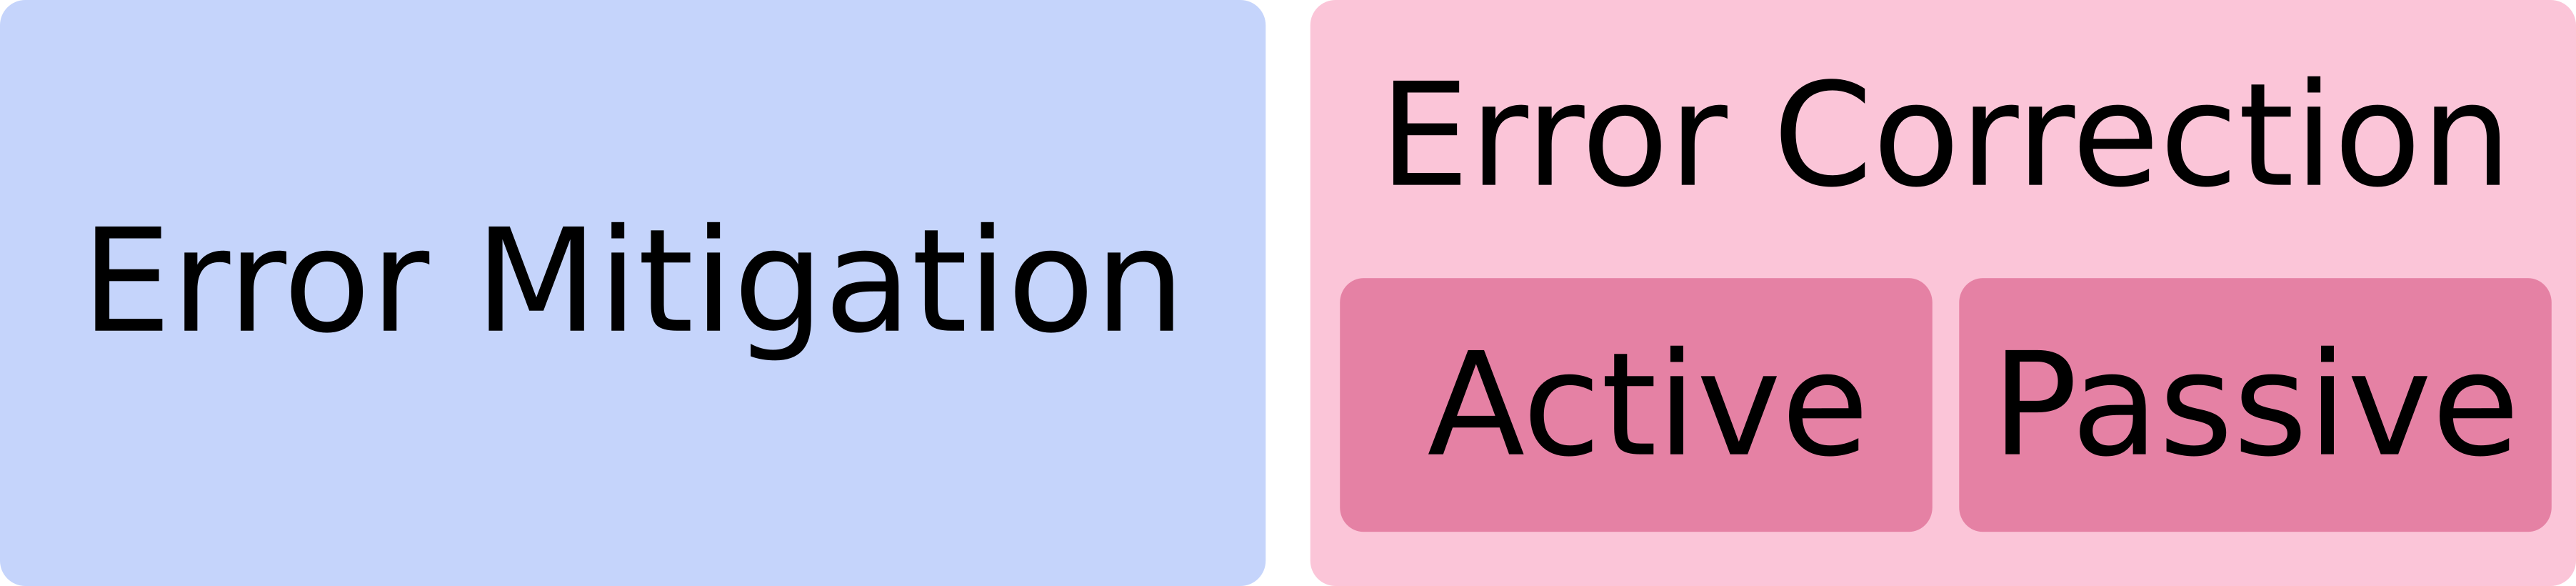
\includegraphics[width=0.6\textwidth]{fig/TypesErrorCorrection.png}
%     \end{center}
% 	\begin{itemize}
% 		\item \textbf{QEM:} Evaluate accurate expectation values of observables on noisy quantum circuits
% 		\item \textbf{QEC:} Build a framework to herald qubits and gates of arbitrary good quality
% 		\begin{itemize}
% 			\item \textbf{Active:} Extracts information about apparent errors and deduces correction operations
% 			\item \textbf{Passive:} Store quantum information in a self correcting way \cite{bacon_operator_2006, berthusen_experiments_2024}
% 		\end{itemize}
% 	\end{itemize}
% \end{frame}

% \begin{frame}{Tackling Quantum Errors}
% 	\begin{center}
%         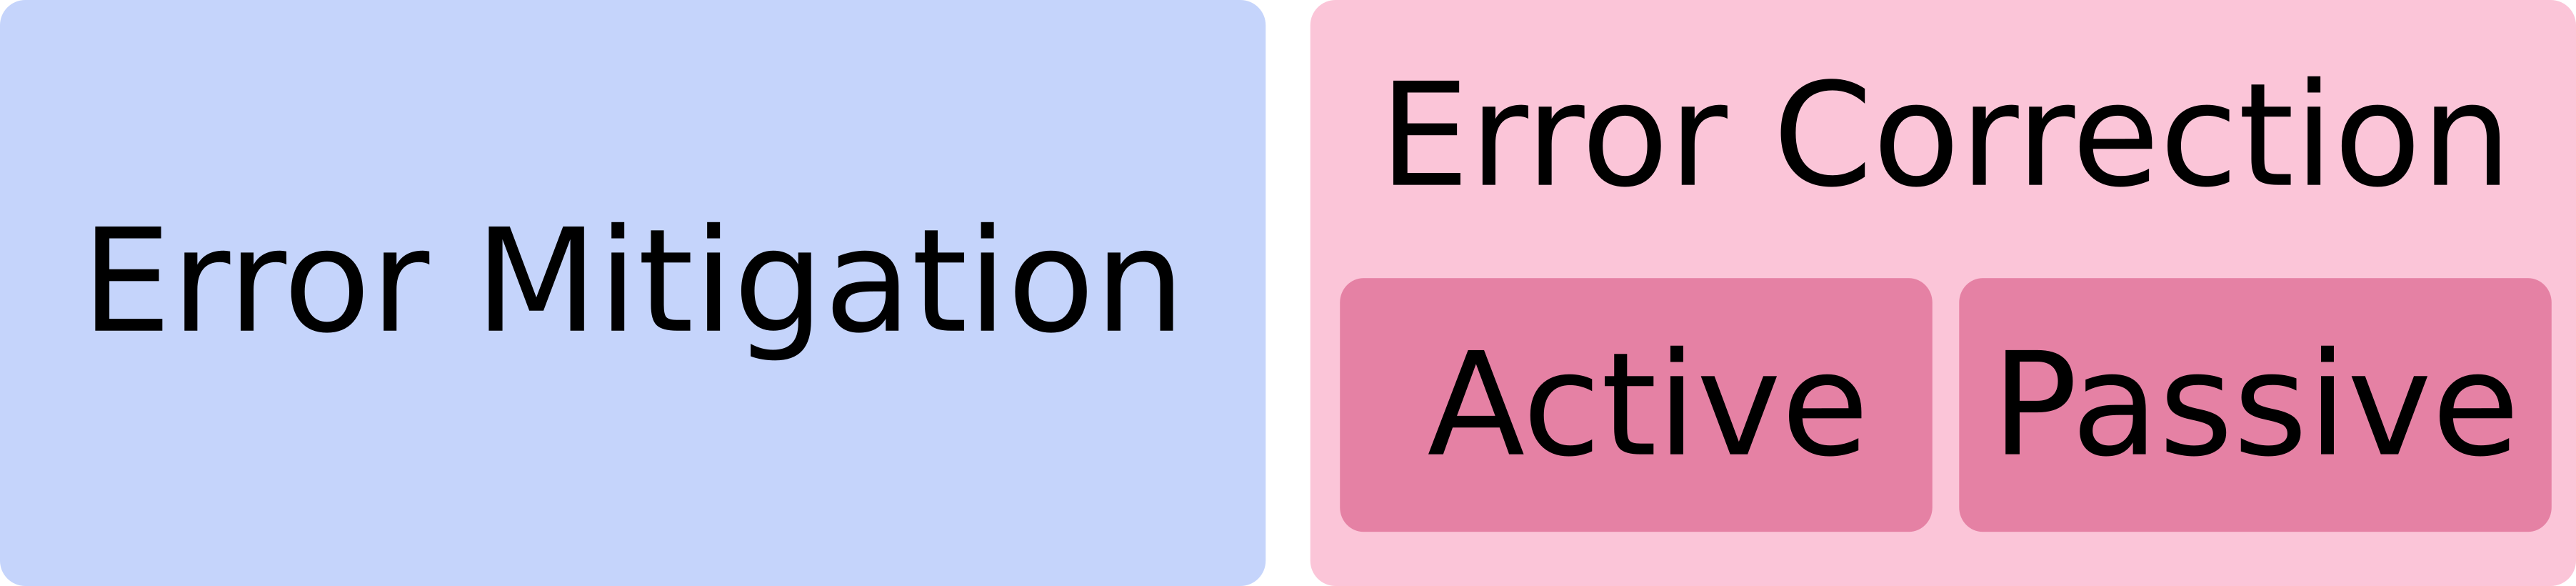
\includegraphics[width=0.6\textwidth]{fig/TypesErrorCorrection.png}
%     \end{center}
% 	\begin{itemize}
% 		\item \textbf{QEM:} Evaluate accurate expectation values by noisy quantum circuits
% 		\item \textbf{QEC:} Obtain qubits and gates of arbitrary good quality
% 		\begin{itemize}
% 			\begin{tcolorbox}[colback=osakared!5!white, colframe=osakared, width=13cm, arc=2mm]
% 			\item \textbf{Active:} Relies on actively measuring information about errors and deducing correction operations
% 			\end{tcolorbox}
% 			\item \textbf{Passive:} Store quantum information in a self correcting way~\cite{bacon_operator_2006, berthusen_experiments_2024}
% 		\end{itemize}
% 	\end{itemize}
% \end{frame}

\begin{frame}{QEC general idea}
	\begin{minipage}[t]{0.65\textwidth}
		\centering
		\textbf{Error correction code:}
		\hspace{1cm}
		\raisebox{-0.3cm}{
\includegraphics[width=0.15\textwidth]{fig/single_qubit.png}}
		\hspace{1cm}
		$\hat{=}$
		\hspace{1cm}
	\end{minipage}
	\begin{minipage}[t]{0.3\textwidth}
		\vspace{-1.5cm}
        
\includegraphics[width=0.6\textwidth]{fig/error_correction_code.png}
    \end{minipage}
	\pause
	\begin{tikzpicture}[overlay]
        \draw[-, line width=0.8mm, osakared] (-3.2, -1.2) -- (-3.2, -1.6);
        \draw[-, line width=0.8mm, osakared] (-3.17, -1.6) -- (-10.03, -1.6);
        \draw[->, line width=0.8mm, osakared] (-10, -1.6) -- (-10, -3.5);
    \end{tikzpicture}
	\begin{tikzpicture}[overlay]
        \draw[<-, line width=0.8mm, osakared] (-2.5, -1.2) -- (-2.5, -3.5);
    \end{tikzpicture}
	\par
	\vspace{1.5cm}
	\hspace{0.8cm}
	\textbf{Decoder:}
	\vspace{-1cm}
	\begin{center}
		Partial error information
		\hspace{0.5cm}
		\raisebox{-5pt}{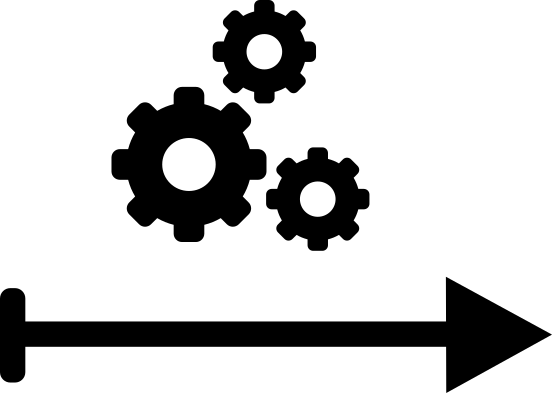
\includegraphics[width=0.2\textwidth]{fig/classical_algorithm.png}}
		\hspace{0.5cm}
		correction operation
	\end{center}
	\pause
	\only<3-3>{
		\begin{textblock*}{3.5cm}(1cm,4cm)
			\begin{tcolorbox}[colback=osakared!5!white, colframe=osakared, width=4cm, arc=2mm]
				\center
				Backlog problem
			\end{tcolorbox}
		\end{textblock*}
	}
\end{frame}

\begin{frame}{Scaling the system size}
	\vspace{10pt}
	\begin{center}
		
\includegraphics[width=0.12\textwidth]{fig/error_correction_code.png}
		\begin{tikzpicture}[overlay]
			\draw[->, line width=0.8mm, osakared] (1, 1) -- (8,1)
			node[midway, above, yshift=15pt, text=black] {Probability of error appearance increases}
            node[midway, below, yshift=-15pt, text=black] {Redundancy increases robustness of logical qubit};
		\end{tikzpicture}
		\hspace{9cm}
        
\includegraphics[width=0.12\textwidth]{fig/scaling_system_size.png}
	\end{center}
	\pause
	\begin{center}
		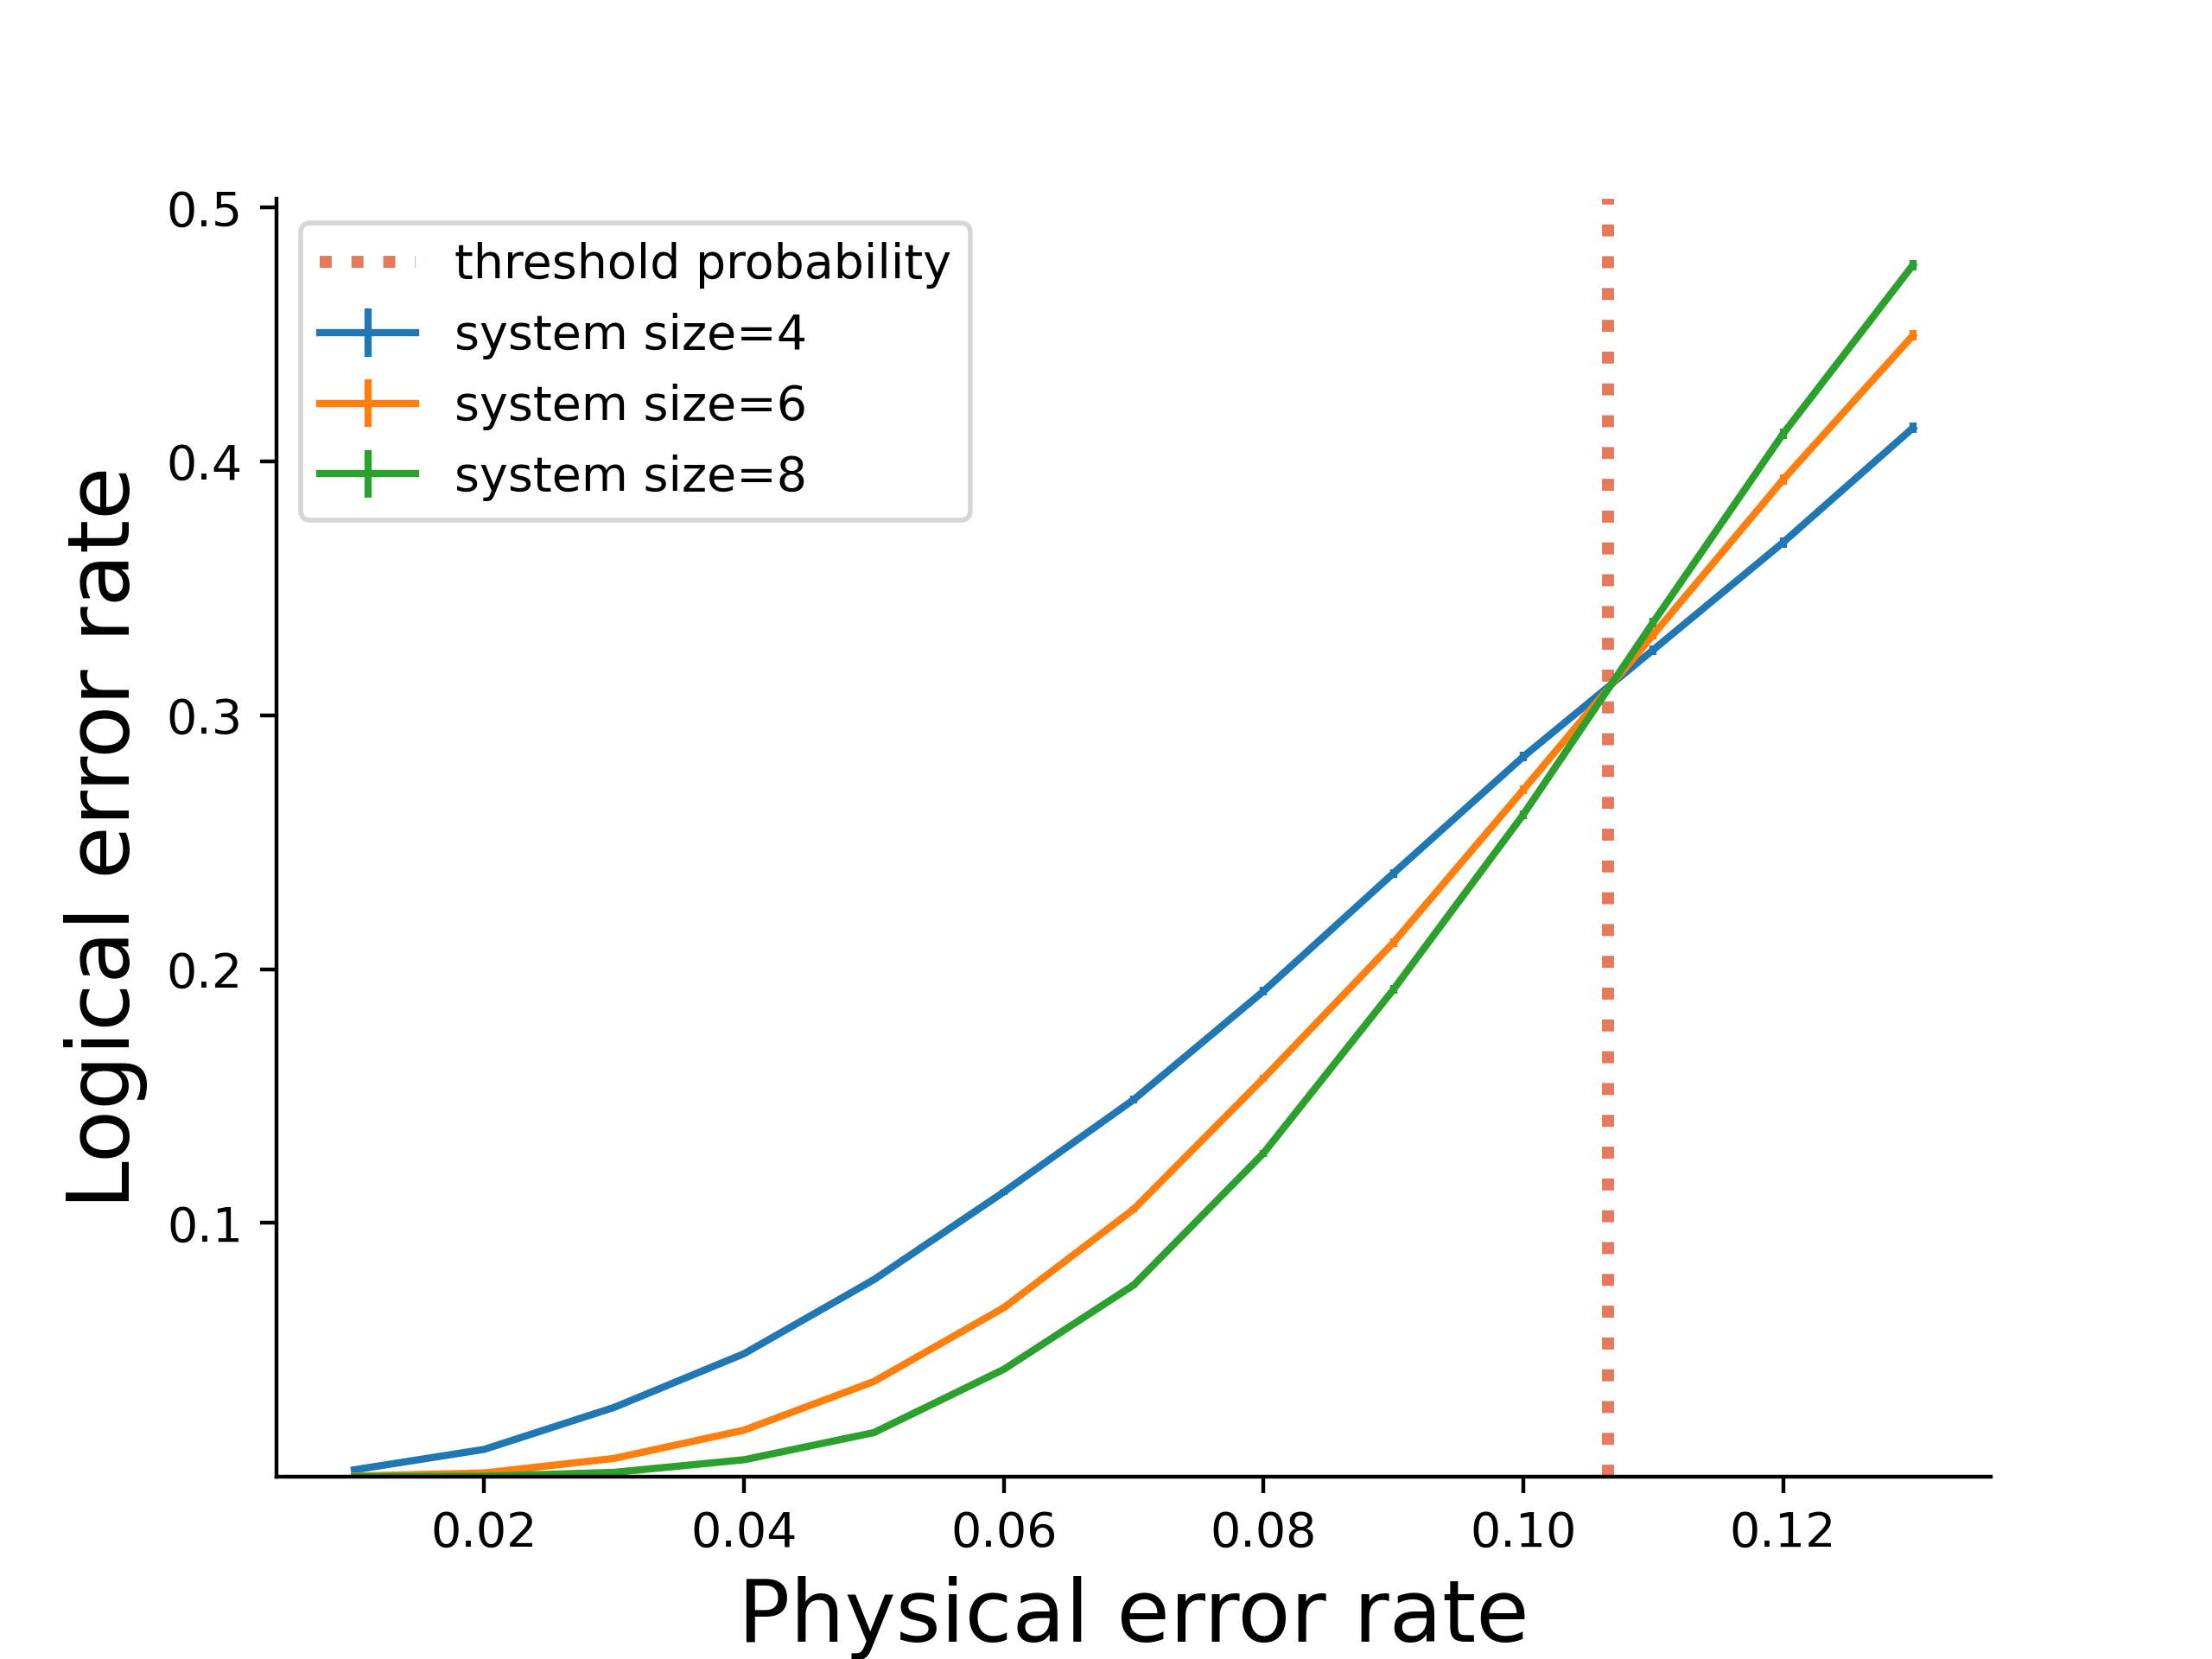
\includegraphics[width=0.4\textwidth]{fig/threshold.png}
		\hspace{0.5cm}
		\pause
        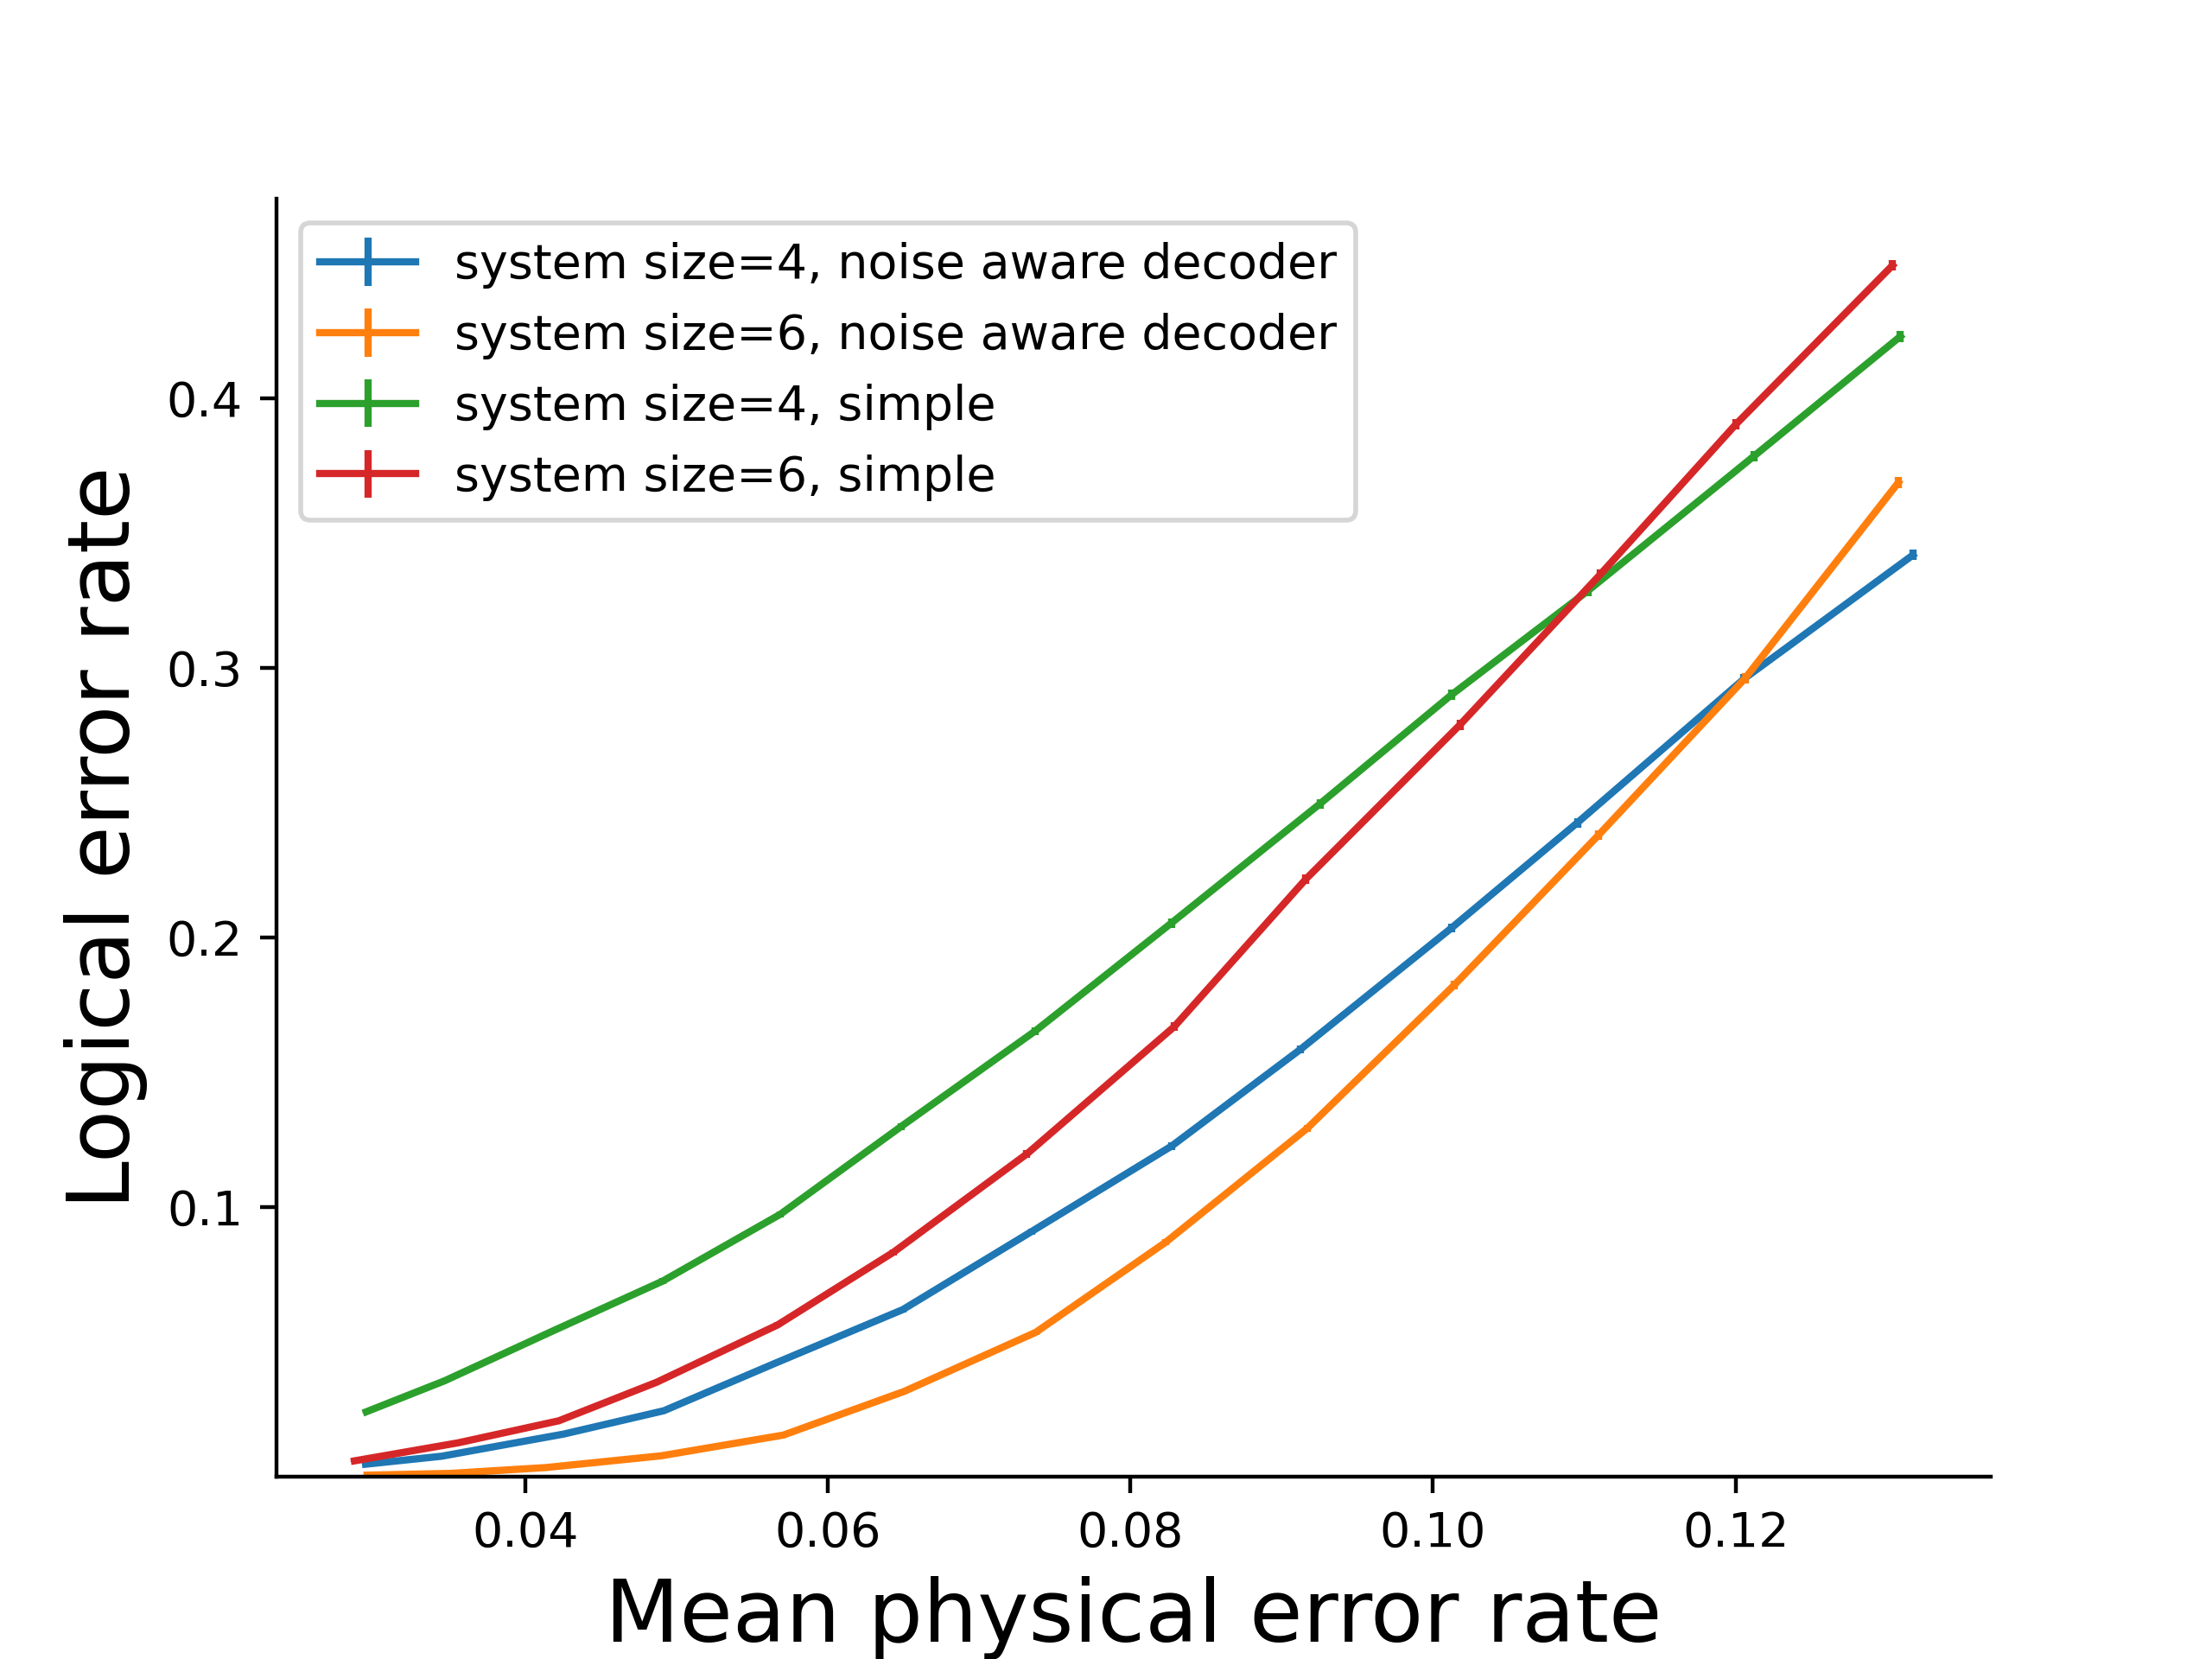
\includegraphics[width=0.4\textwidth]{fig/noise_aware.png}
	\end{center}
	% With an increase of physical qubits the probability that an error occurs increases, too. This effect is countered by an increase in robustness of logical qubits towards noise with increased qubit counts.
	% This interplay lets us distinguish two regimes: Below a characteristic physical error rate, the logical qubit noise is suppressed by qubit count increasement.
	% Above this specific error probability, the logical qubit noise increases with the number of qubits.\\
	% The error rate seperating these two regimes is called the error correction threshold.
\end{frame}

\begin{frame}{Problem statement}
	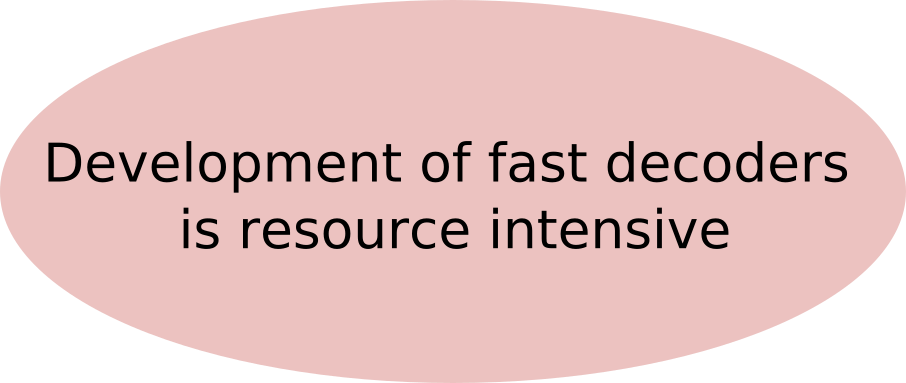
\includegraphics[width=0.4\textwidth]{fig/resource_intensive_decoder_dev.png}
	\only<1>{\hspace{20pt}\raisebox{35pt}{$\huge \Rightarrow$ \textbf{Only do it for promising codes}}}
	\only<2->{
		\hspace{2pt}
		\raisebox{18pt}{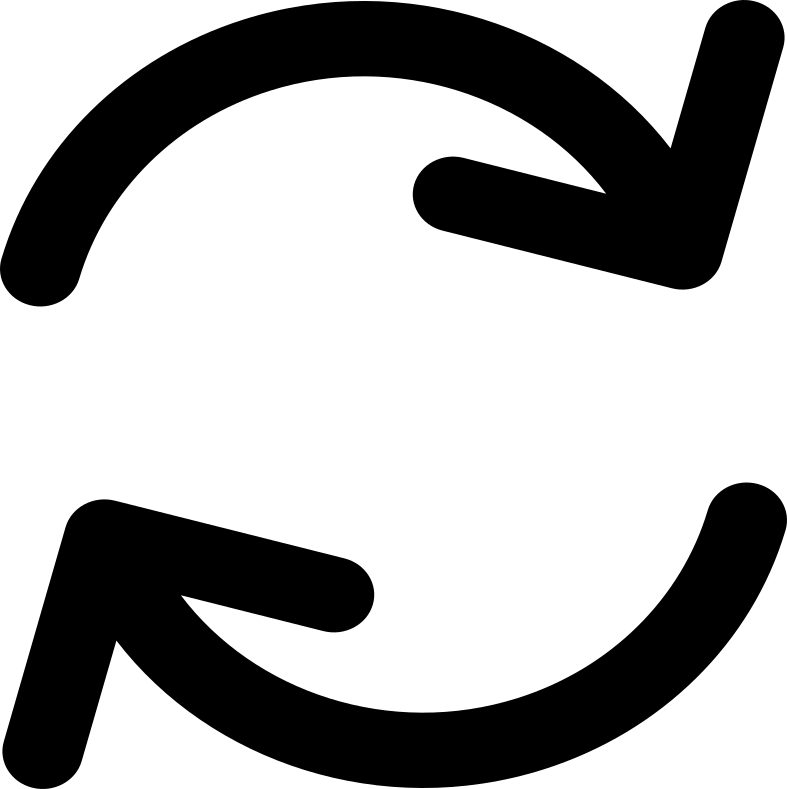
\includegraphics[width=0.08\textwidth]{fig/arrows.png}}
		\hspace{5pt}
		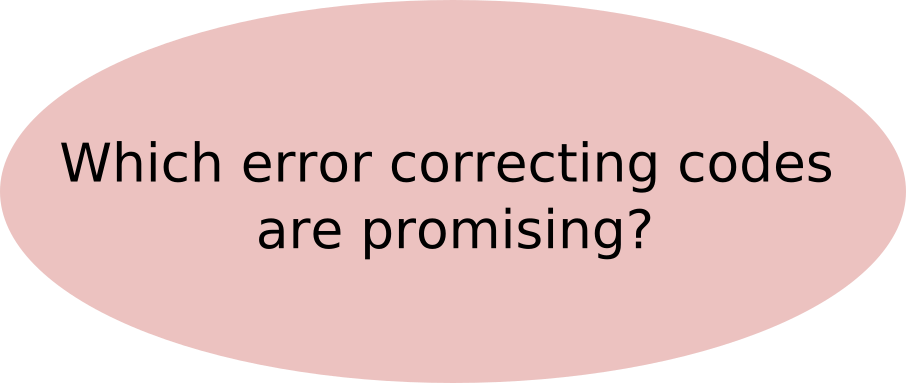
\includegraphics[width=0.4\textwidth]{fig/promising_codes.png}\\
	}
	\vspace{1.5cm}
	\only<3->{
	\center
	\textbf{Optimal code performance: \\baseline for code selection and decoder optimization}
	% \begin{itemize}
	% 	\only<3->{\item \textbf{Code selection:} Hardware specific simulation of optimal code performance makes error correcting codes comparable.}
	% 	\only<4>{\item \textbf{Decoder optimization:} Estimation of optimal code performance shows upper limit for decoder optimization.}
	% \end{itemize}
	}
\end{frame}

% \begin{frame}{Noise}
% 	\begin{center}
%         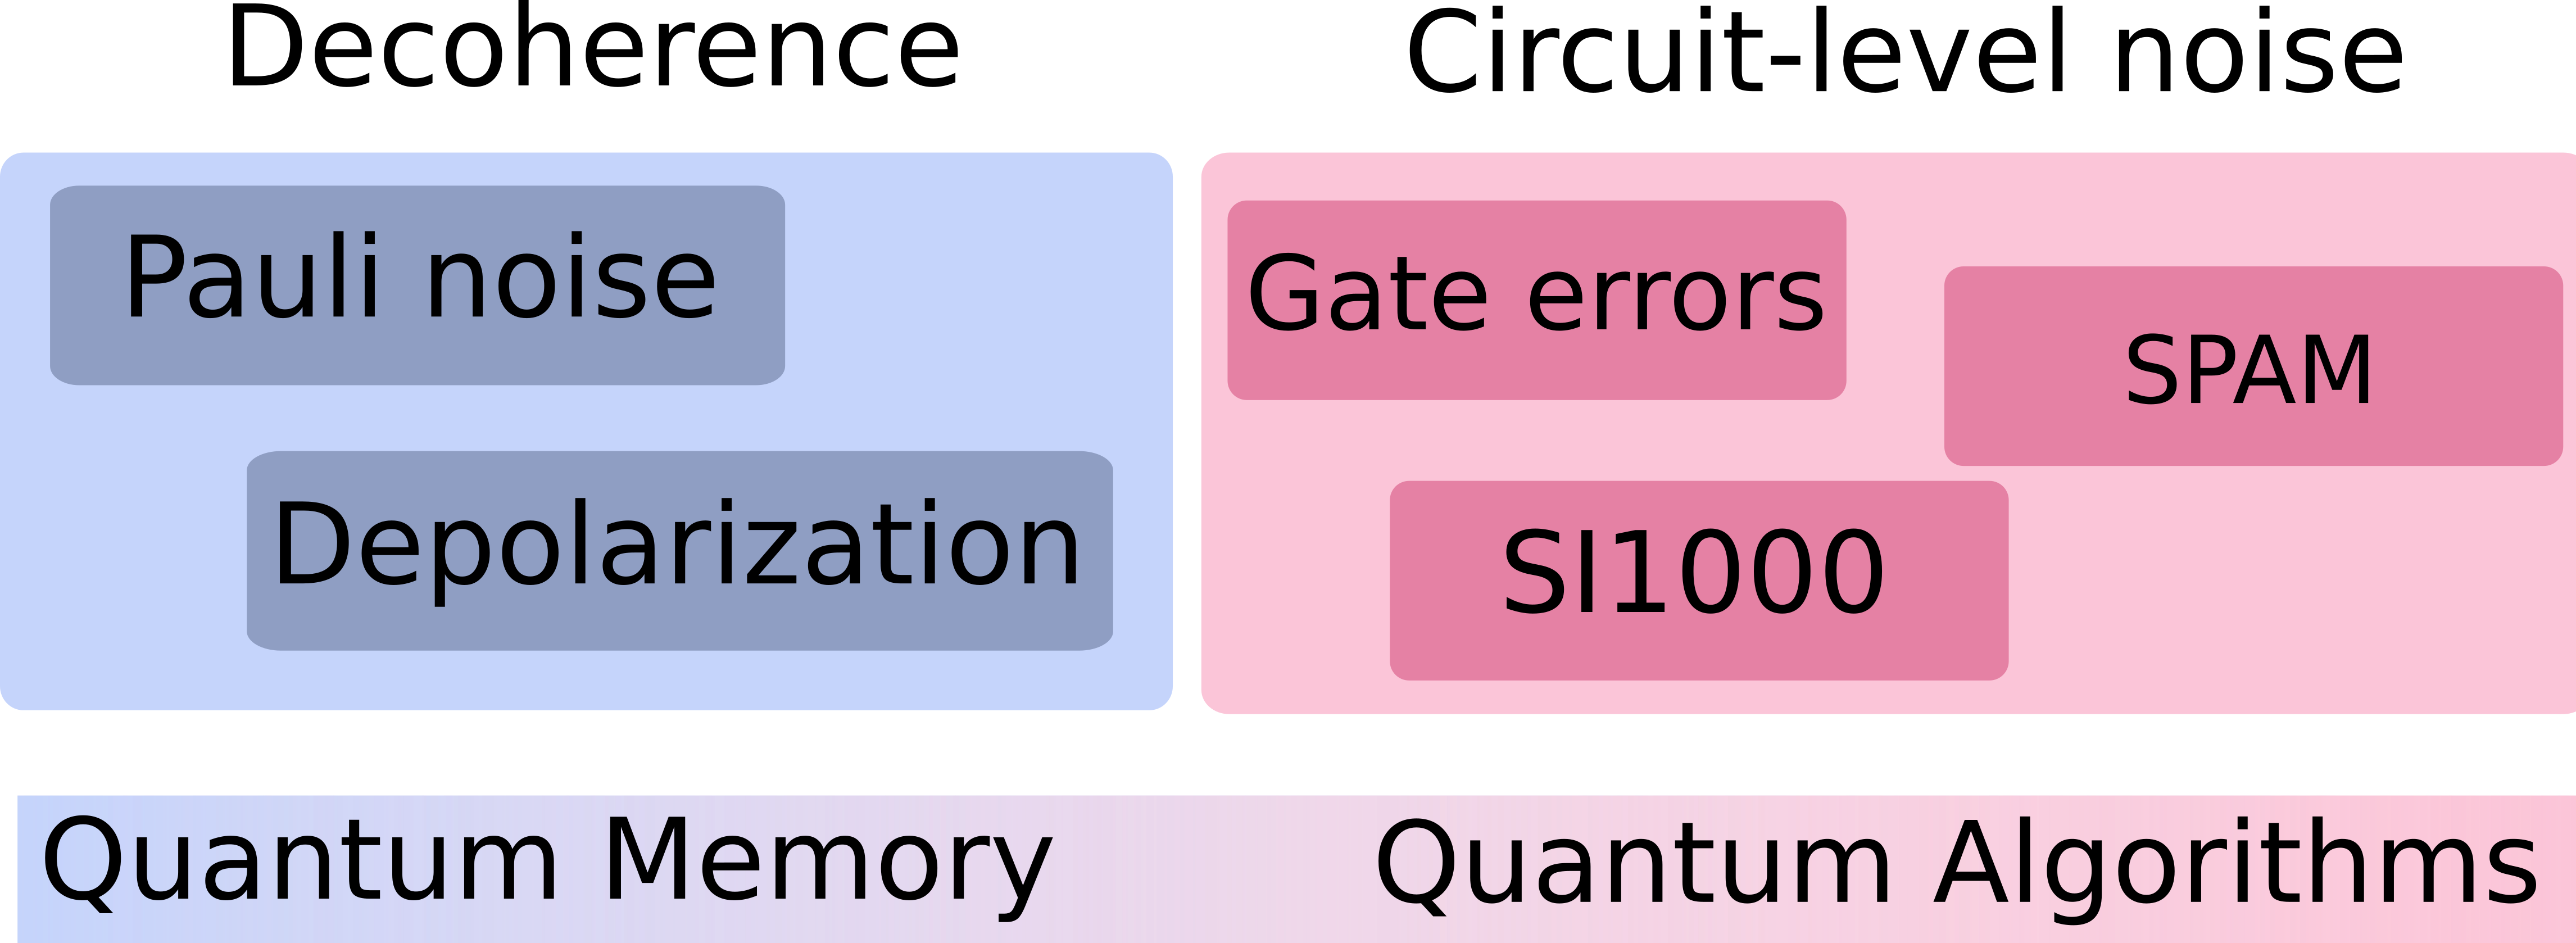
\includegraphics[width=0.6\textwidth]{fig/NoiseTypes.png}
%     \end{center}
% 	\small
% 	\begin{itemize}
% 		\item \textbf{Decoherence:} Interaction with environment evolves idle qubit states stochastically
% 		\item \textbf{Circuit-level Noise:} Caused by imperfect manipualtion of QI:
% 		\begin{itemize}
% 			\item Imperfect implementation of quantum gates causes errors
% 			\item \textbf{S}tate \textbf{P}reparation \textbf{A}nd \textbf{M}easurement errors
% 			\item SI1000: \textbf{S}uperconducting \textbf{I}nspired noise model with \textbf{1000} nanosecond cycle
% 		\end{itemize}
% 	\end{itemize}
% 	\pause
% 	\begin{overlayarea}{\textwidth}{3cm}
% 	\vspace{-8cm}
% 	\hspace{3.5cm}
% 	\begin{tikzpicture}
% 		% Define nodes
% 		\node (A) at (0cm,0cm) {};
% 		\node (B) at (6cm,0cm) {};
% 		\node (C) at (4cm,0cm) {};

% 		% Draw a curved arrow from B to A
% 		\draw[->, bend right=40] (B) to node[above] {Pauli Twirl \cite{geller_efficient_2013}} (A);
% 		\draw[->, bend right=25] (C) to node[above] {} (0.5cm, 0cm);
% 	\end{tikzpicture}
% 	\end{overlayarea}
% \end{frame}


% \begin{frame}{Overview Literature Research}
% 	\begin{center}
% 		\begin{itemize}
% 			\only<1->{
% 			\item Optimal code capacity thresholds
% 			}
% 			\vspace{0.5cm}
% 			\pause
% 			\only<2->{
% 			\item Surface code decoders
% 			}
% 			\vspace{0.5cm}
% 			\pause
% 			\only<3->{
% 			\item Noise effects on code performance
% 			}
% 		\end{itemize}
% 	\end{center}
% \end{frame}


% \begin{frame}{Brief history of QEC}
% 	\vspace{-20pt}
% 	\begin{table}[h]
%         \centering
% 		\renewcommand{\arraystretch}{1.5}
%         \resizebox{\textwidth}{!}{
% 		\begin{tabular}{c|c|p{7cm}}
% 			\textbf{Year} & \textbf{Author} & \textbf{Contribution} \\
% 			1995 & Shor & First quantum error correcting code and threshold theorem~\cite{shor_scheme_1995} \\
% 			1996 & Calderbank, Shor and Steane & Introduction of quantum error correcting codes based on classical codes~\cite{calderbank_good_1996, steane_multiple-particle_1996} \\
% 			1997 & Gottesman & Introduction of stabilizer code framework~\cite{gottesman_stabilizer_1997} \\
% 			1997 & Kitaev & Introduction of the surface code~\cite{hirota_quantum_1997, kitaev_fault-tolerant_2003}\\
% 			2002 & Dennis, Kitaev, Landahl and Preskill & Introduction of statistical mechanics mapping and fault tolerant operations on the surface code~\cite{dennis_topological_2002} \\
% 			2014-15 & Nigg et al. and  Kelly et al. & First experimental realization of small codes \cite{nigg_quantum_2014,kelly_state_2015} \\
% 		\end{tabular}
% 		}
% 	\end{table}
% \end{frame}


% \begin{frame}{Stabilizer Codes}
% 	% \begin{textblock*}{2.5cm}(12.5cm,0.5cm)
% 	% 	
\includegraphics[width=1\textwidth]{fig/QEC_pure_code.png}
% 	% \end{textblock*}
% 	Quality markers: $\frac{k}{n}$, d (, $\omega$ for QLDPC)
% 	\begin{table}[h]
%         \renewcommand{\arraystretch}{1.5} % Increase row spacing
%         \small
% 		\begin{tabular}{c|c|c|c}
% 			\textbf{Code} &  \textbf{n} & \textbf{k} & \textbf{d} \\
% 			\hline
% 			Toric Code \cite{hirota_quantum_1997} & $2d^{2}$ & 2 & d \\
% 			Planar Surface Code & $d^{2} + (L-1)^{2}$ &  1 & d \\
% 			Rotated Surface Code & $d^{2}$ &  1 & d \\
% 			\hline
% 			\pause
% 			Honneycomb Code \cite{landahl_fault-tolerant_2011} & $\frac{3}{4}d^{2}$ + $\frac{1}{4}$ & 1 & d \\
% 			\hline
% 			\pause
% 			Quantum Tanner Code \cite{leverrier_quantum_2022} & n & $\Omega(n)$ & $\Omega(n)$
% 		\end{tabular}
% 	\end{table}
% \end{frame}


\begin{frame}{Optimal Code Capacity Thresholds}
	Quality marker: $p_{\text{threshold}}$
	\begin{table}[h]
        \renewcommand{\arraystretch}{1.5} % Increase row spacing
        \small
		\begin{tabular}{c|c|c}
			\textbf{Code} & \textbf{Noise} & \textbf{Publications} \\
			\hline
			Toric Code & Independent X, Z errors & \cite{merz_two-dimensional_2001, honecker_nishimori_2001} \\
			 & Depolarizing Noise & \cite{bombin_strong_2012} \\
			 & Correlated Noise & \cite{chubb_statistical_2019}\\
			\hline
			Surface Code & Independent X, Z errors & \cite{bravyi_efficient_2014} \\
			& Depolarizing Noise & \cite{bravyi_efficient_2014} \\
			& Amplitude Damping & \cite{darmawan_tensor-network_2017} \\
			& Coherent Noise & \cite{behrends_statistical_2024, bao_phases_2024}
		\end{tabular}
	\end{table}
	% \pause
	% \only<2-2>{
	% 	\begin{textblock*}{4cm}(12.5cm,2.5cm)
	% 		\small
	% 		Optimal decoding threshold $\sim$ phase transition at Nishimori temperature
	% 	\end{textblock*}
	% }
\end{frame}


\begin{frame}{Surface Code Suboptimal Decoders}
	% \begin{textblock*}{2cm}(14cm,0.5cm)
	% 	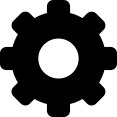
\includegraphics[width=0.4\textwidth]{fig/decoder.png}
	% \end{textblock*}
	\begin{textblock*}{9cm}(7cm,2.5cm)
        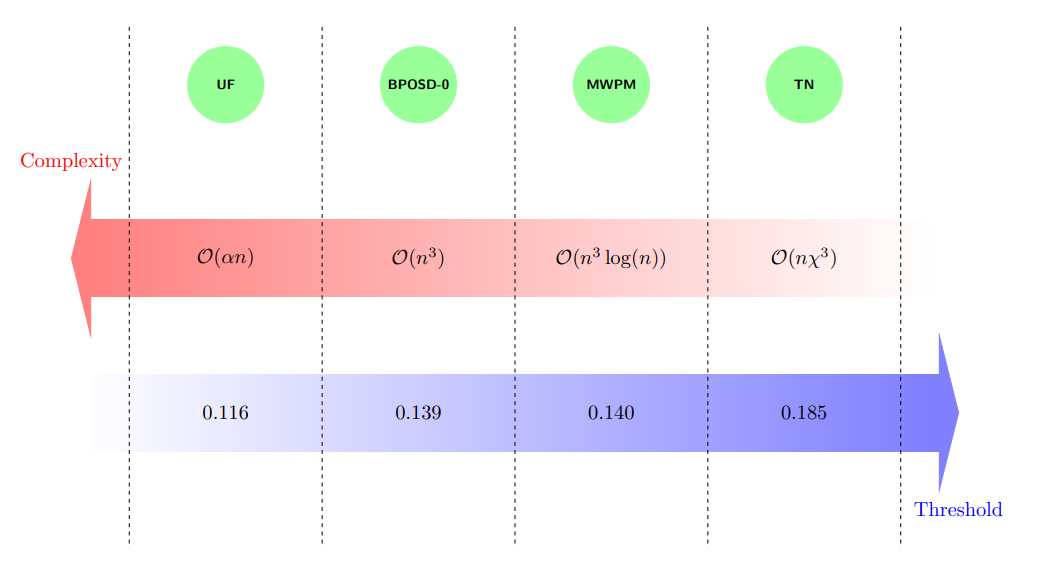
\includegraphics[width=1\textwidth]{fig/Screenshot from 2025-03-24 15-21-55.png}
    \end{textblock*}
	\begin{textblock*}{2cm}(12.5cm,3.4cm)
		\begin{tiny}
			\cite{edmonds_paths_1965}
		\end{tiny}
	\end{textblock*}
	\begin{textblock*}{2cm}(9.2cm,3.4cm)
		\begin{tiny}
			\cite{delfosse_almost-linear_2021}
		\end{tiny}
	\end{textblock*}
	\begin{textblock*}{2cm}(10.8cm,3.4cm)
		\begin{tiny}
			\cite{panteleev_degenerate_2021}
		\end{tiny}
	\end{textblock*}
	\begin{textblock*}{2cm}(14.1cm,3.4cm)
		\begin{tiny}
			\cite{bravyi_efficient_2014,chubb_general_2021}
		\end{tiny}
	\end{textblock*}

	\only<1-1>{
		\begin{textblock*}{3.5cm}(1cm,4cm)
			\begin{tcolorbox}[colback=osakared!5!white, colframe=osakared, width=4cm, arc=2mm]
				\center
				Backlog problem
			\end{tcolorbox}
		\end{textblock*}
	}
	% \pause
	% \only<2-2>{
	% \begin{textblock*}{5.8cm}(0.1cm,3.5cm)
	% 	\begin{small}
	% 	\textbf{Union Find}
	% 	\begin{itemize}
	% 		\item Pauli errors $\rightarrow$ erasure errors
	% 		\item almost linear time complexity
	% 		\item Noise aware \cite{higgott_improved_2023}
	% 	\end{itemize}
	% 	\end{small}
	% \end{textblock*}
	% }
	% \pause
	% \only<3-3>{
	% \begin{textblock*}{5.8cm}(0.1cm,3cm)
	% 	\begin{small}
	% 	\textbf{Belief Propagation}
	% 	\begin{itemize}
	% 		\item Acts on general Tanner graphs $\rightarrow$ any QLDPC decoder
	% 		\item Issues with highly degenerate codes (split-belief phenomenon) \cite{poulin_iterative_2008, roffe_decoding_2020}
	% 		\item Ordered statistics decoding (BP+OSD) to enhance performance \cite{panteleev_degenerate_2021}
	% 	\end{itemize}
	% 	\end{small}
	% \end{textblock*}
	% }
	\pause
	\only<2-2>{
	\begin{textblock*}{7cm}(0cm,2cm)
		\begin{small}
			\textbf{\hspace{1cm}Minimum Weight Perfect Matching}
			\begin{itemize}
				\item Complexity improved: Sparse blossom $O(N^{1.32})$, fusion blossom $O(N)$
				\item Sparse blossom: Real time decoding $0.1\%$ depolarising noise on distance-17 surface code \cite{higgott_sparse_2025}
				\item Improved performance: Ensembling~\cite{shutty_efficient_2024, jones_improved_2024},
				\item Noise aware: Weights calibrated by noise~\cite{iolius_performance_2022,hockings_improving_2025}, correlated MWPM~\cite{fowler_optimal_2013}
			\end{itemize}
		\end{small}
	\end{textblock*}
	\begin{textblock*}{10cm}(9.7cm,3.5cm)
		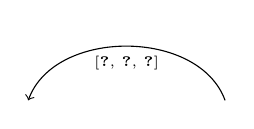
\begin{tikzpicture}
			\draw[->, bend right=70] (2.5cm,0cm) to node[below] {\tiny{\cite{fowler_towards_2012, wu_fusion_2023, higgott_sparse_2025}}} (0cm,0cm);
		\end{tikzpicture}
	\end{textblock*}
	}
	\pause
	\only<3-3>{
	\begin{textblock*}{7cm}(0cm,3cm)
		\begin{small}
			\textbf{\hspace{1cm}Tensor Network Decoder}
			\begin{itemize}
				\item Surface Code $\rightarrow$ Tensor Network
				\item Optimal decoding $\rightarrow$ TN contraction
				\item Approximate contraction $\rightarrow$ approximate optimal decoding
				\item Generalised to arbitrary 2D codes \cite{chubb_general_2021}
				\item Noise aware~\cite{darmawan_optimal_2024}
			\end{itemize}
		\end{small}
	\end{textblock*}
	}
\end{frame}


% \begin{frame}{Experimental Realization}
% 	\vspace{-18pt}
% 	\begin{table}[h]
% 		\fontsize{10pt}{10pt}\selectfont
%         \renewcommand{\arraystretch}{1.5} % Increase row spacing
% 		\begin{tabular}{c|p{3cm}|p{8.5cm}}
% 			\textbf{Year} & \textbf{Author} & \textbf{Contribution} \\
% 			2014 & Nigg et al. & Seven-qubit color code on trapped-ion device and execution of logical single-qubit gates \cite{nigg_quantum_2014} \\
% 			2015 & Kelly et al. &  Nine qubit repetition code on superconducting processor \cite{kelly_state_2015} \\
% 			2020 & Erhard et al. & Lattice surgery generated entanglement of two logical qubits on a ten qubit ion trap device \cite{erhard_entangling_2020} \\
% 			2021 & Ryan et al. & Real time decoding on seven-qubit color code on trapped-ion device and non-Clifford operation \cite{ryan-anderson_realization_2021}\\
% 			2023-24 & Google Quantum AI et al. & Real time decoding and below threshold quantum memory experiments on up to 101 qubits on superconducting processor \cite{google_quantum_ai_suppressing_2023, google_quantum_ai_and_collaborators_quantum_2025}
% 		\end{tabular}
% 	\end{table}
% \end{frame}

% \begin{frame}{Optimal Decoding Methods}
% 	\vspace{-15pt}
% 	\begin{table}[h]
%         \renewcommand{\arraystretch}{1.5} % Increase row spacing
%         \small
% 		\begin{tabular}{c|p{4cm}|p{7cm}}
% 			\textbf{Year} & \textbf{Author} & \textbf{Contribution} \\
% 			2009 & Creighton and Middleton \cite{thomas_exact_2009,thomas_numerically_2013} & Fast algorithm to calculate finite temperature partition functions of planar random bond Ising model based on FKT algortihm \cite{kasteleyn_statistics_1961,temperley_dimer_1961} \\
% 			2013 & Vogel, Li, Wüst, Landau \cite{vogel_generic_2013} & Parallel tempered Wang-Landau algorithm \cite{wang_efficient_2001} for estimating density of states for systems with bounded spectrum \\
% 			2014-21 & Bravyi, Suchara, Vargo and Chubb \cite{bravyi_efficient_2014, chubb_general_2021} & Development of approximate optimal decoding by TN contraction and generalisation to arbitrary 2D stabiliser codes \\
% 		\end{tabular}
% 	\end{table}
% \end{frame}

\begin{frame}{Gap}
	Existing:
	\begin{itemize}
		\item Much effort in development of error correcting codes with good quality markers: Number logical per physical qubits, code distance and $p_{\text{threshold}}$
		\item Much effort in development of fast and high performant decoders for stabilizer codes
	\end{itemize}
	\pause
	Laking:
	\begin{itemize}
		\item Comparibility of codes for finite size regime under realistic noise models
		\item Gauge of existing decoders with respect to optimal code capacity
	\end{itemize}

\end{frame}
\begin{frame}{Research goal}
	Development of hardware adaptive framework:
	\begin{center}
		\raisebox{-0.5cm}{
\includegraphics[width=0.15\textwidth]{fig/Noise.png}}
		\begin{tikzpicture}[overlay]
			\draw[->, line width=0.8mm, black] (0.5, 0.1) -- (4,0.1);
			\draw[-, line width=0.8mm, black] (0.5, 0.3) -- (0.5,-0.1);
		\end{tikzpicture}
		\hspace{4.5cm}
		Optimal code performance estimate
	\end{center}\vspace{20pt}

	\begin{itemize}
		\item Informed decision on which codes promise good finite size performance
		\item Gauge of decoder optimization process
	\end{itemize}
\end{frame}

\begin{frame}{Research plan}
	\begin{table}[h]
        \renewcommand{\arraystretch}{1.5} % Increase row spacing
        \small
		\begin{tabular}{c|p{10cm}}
			\textbf{Time} &  \textbf{Objective} \\
			\hline
			Now & Framework for general stabilizer code under Pauli noise is implemented \\
			April-May 2025 & Paper on optimization opportunities of MWPM by degeneracy of ground states \\
			May- 2025 & Incoroporate TN approximate ML decoder into framework plus investigate further alternatives \\
			May- 2025 & Incorporate realistic circuit level noise model into framework by Pauli twirling and investigate its influence \\
			2025-2026 & Implementation of error correcting codes, deduction of noise model and simulation of hardware within QuaSA\\
		\end{tabular}
	\end{table}
\end{frame}

\begin{frame}{Preliminary Results}
	\only<1-1>{
	\begin{textblock*}{14cm}(1.5cm,2cm)
		\raisebox{-0.5cm}{
\includegraphics[width=0.15\textwidth]{fig/Noise.png}}
		\begin{tikzpicture}[overlay]
			\draw[->, line width=0.8mm, black] (0.5, 0.1) -- (4,0.1);
			\draw[-, line width=0.8mm, black] (0.5, 0.3) -- (0.5,-0.1);
		\end{tikzpicture}
		\hspace{4.5cm}
		Optimal code performance estimate
	\end{textblock*}
	}
	\pause
	\only<2->{
	\begin{textblock*}{14cm}(1.5cm,2cm)
		\raisebox{-0.7cm}{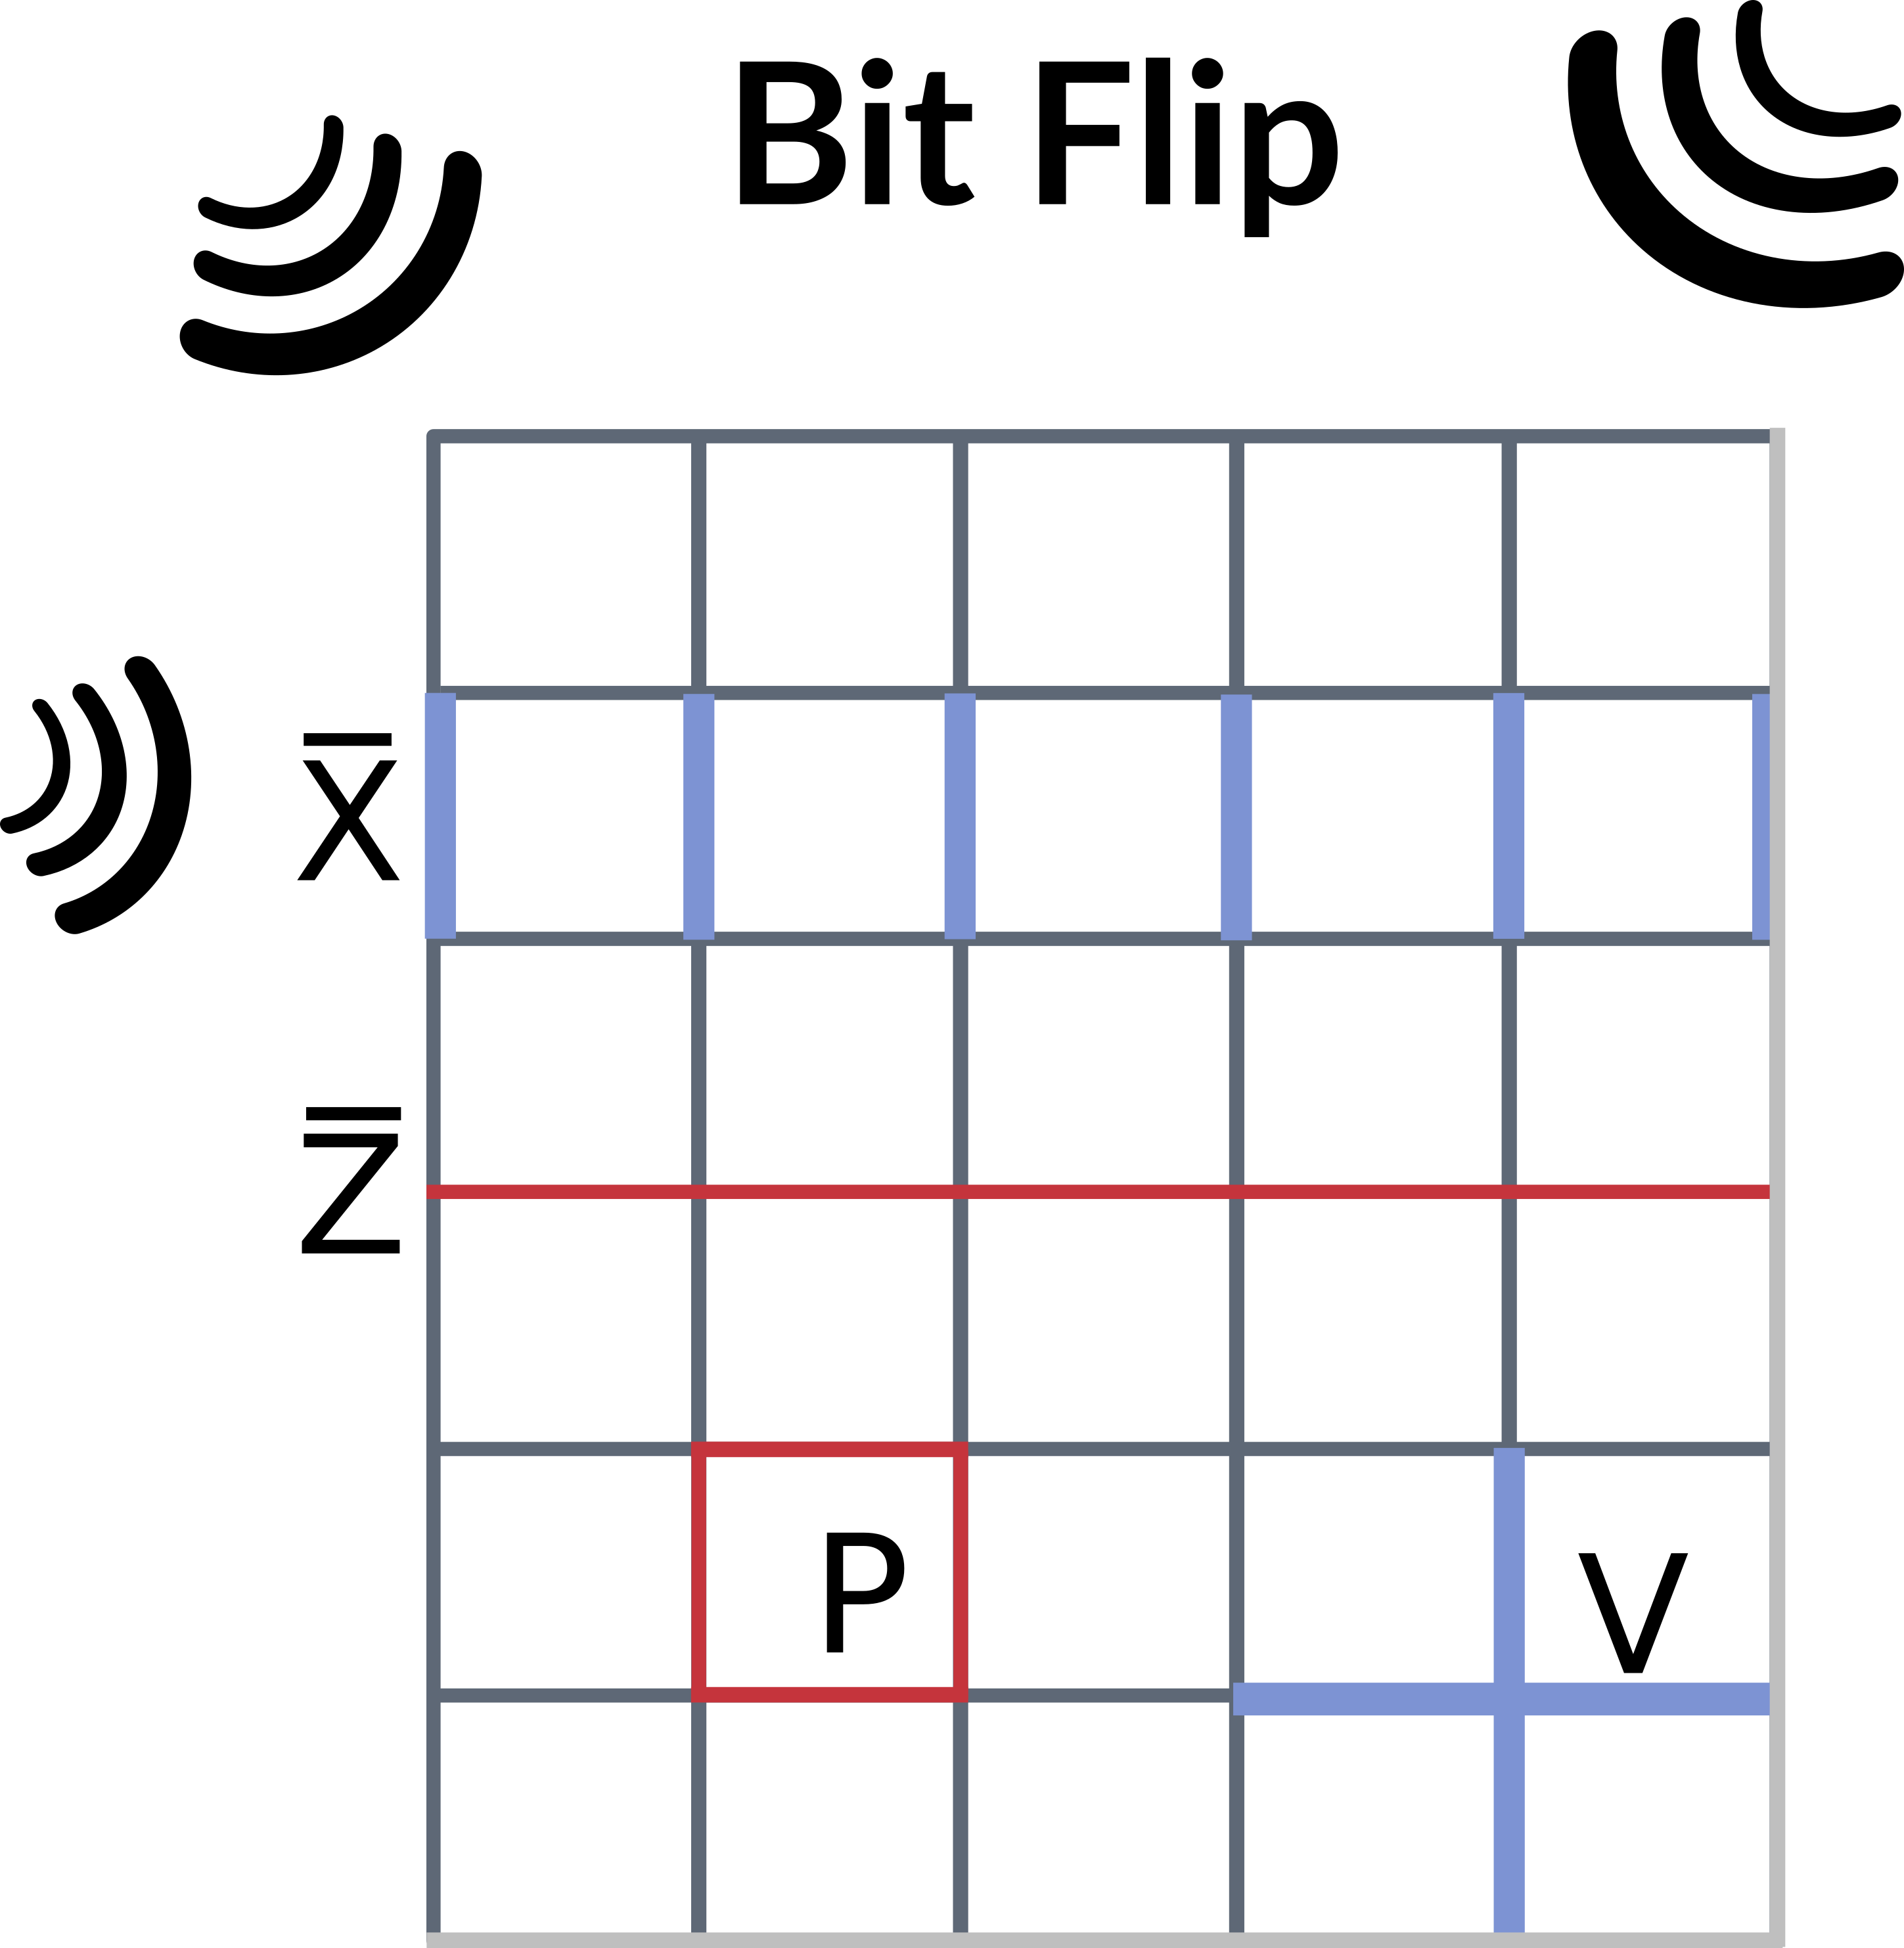
\includegraphics[width=0.15\textwidth]{fig/toric_code.png}}
		\begin{tikzpicture}[overlay]
			\draw[->, line width=0.8mm, black] (0.5, 0.1) -- (4,0.1);
			\draw[-, line width=0.8mm, black] (0.5, 0.3) -- (0.5,-0.1);
		\end{tikzpicture}
		\hspace{4.5cm}
		Error class probability estimates
	\end{textblock*}
	}
	% \pause
	% \only<3->{
	% 	\vspace{2cm}
	% 	\hspace{1.5cm}
	% 	\begin{itemize}
	% 		\item Maximum Z decoding $\sim$ decoding probability
	% 		\item Probabilistic Z decoding $\sim$ order probability
	% 		\item Decoding probability and order probability require less samples for same accuracy than respective Z decoding
	% 		\item At low temperature: Order probability $\sim$ maximum probability decoding and decoding probability $\sim$ degeneracy enhanced maximum probability decoding
	% 		\item Enhancing MWPM by takign degeneracy into account can approximate decoding probability
	% 	\end{itemize}
	% }
\end{frame}

\begin{frame}{Groundwork for Results}
\textbf{Example:}
\begin{itemize}
	\item Physical errors $E_{1}, E_{2}, E_{3}$ compatible with partial error information $s$\\
	\pause
	\item $E_{2}, E_{3}$ act equivalently on logical qubit while $E_{1}$ does not\\
	\pause
	\item $P(E_{1})=4\%$, $P(E_{2})=3\%$, $P(E_{3})=3\%$
\end{itemize}
\pause
\vspace{0.5cm}
\textbf{Maximum Probability decoding:}\\
Select most probable physical error consistent with the partial error information\\
\pause
$P(E_{1})\geq P(E_{i})\forall i \Rightarrow$ Select error $E_{1}$\\
\pause
\vspace{0.5cm}
\textbf{Maximum likelihood/Optimal decoding:}\\
Select most probable error class consistent with the partial error information\\
\pause
$P([E_{2}])=P(E_{2})+P(E_{3})> P(E_{1})\Rightarrow$ Select error class $[E_{2}]=[E_{3}]$
\end{frame}

\begin{frame}{Groundwork for Results}
	\only<1-1>{
	\textbf{Maximum Probability decoding:}\\
	Select error consistent with the partial error information and highest $P(E)$\\
	}
	\pause
	\only<2-3>{
	\textbf{Maximum Probability/Minimum Weight decoding:}\\
	Select error consistent with the partial error information and highest $P(E)$\\
	}
	\pause
	\only<3-3>{
	\vspace{0.5cm}
	\textbf{Maximum likelihood/Optimal decoding:}\\
	Select class consistent with the partial error information and highest $P([E])$
	}
	\pause
	\only<4-4>{
		Reduce calculation of $P(E)$ and $P([E])$ to very well studied quantity called partition function $Z_{E}(T)$.\\
	}
	\pause
	\only<5-5>{
		\textbf{Maximum Probability/Minimum Weight decoding:}\\
		Select error consistent with the partial error information and highest $P(E)=lim_{T\to 0}Z_{E}(T)$\\
		\vspace{0.5cm}
		\textbf{Maximum likelihood/Optimal decoding:}\\
		Select class consistent with the partial error information and highest $P([E])=Z_{E}(T_{\text{Nishimori}})$
	}
	\pause
	\only<6->{
		\textbf{Minimum Energy Decoding:}\\
		Select error consistent with the partial error information and highest $P(E)=lim_{T\to 0}Z_{E}(T)$\\
		\vspace{0.5cm}
		\textbf{Maximum Z Decoding:}\\
		Select class consistent with the partial error information and highest $P([E])=Z_{E}(T_{\text{Nishimori}})$
	}
\end{frame}

\begin{frame}{Intermezzo - Groundwork for Results}
    \begin{minipage}{0.48\textwidth}
        \small
		\textbf{Minimum Energy decoding}
		Order probability is estimator of success rate
		\begin{align*}
			&P_{\text{success}}=\lim_{T \to 0}\langle\frac{Z^{T}(E)}{\sum_{l\in L}Z^{T}(l)}\rangle_{s}
		\end{align*}
		with $P(\bar{l}=l)=\frac{Z^{T}(C_{s}L_{l})}{\sum_{l\in L}Z^{T}(C_{s}L_{l})}$
    \end{minipage}
	\pause
	\begin{minipage}{0.48\textwidth}
		\small
		\textbf{Max Z decoding}
		\begin{align*}
			&P_{\text{success}}=\langle\frac{Z^{T_{\text{Nishimori}}}(C^{\star}_{s})}{\sum_{l\in L}Z^{T_{\text{Nishimori}}}(C^{\star}_{s}L_{l})}\rangle_{s}
		\end{align*}
		with $[C^{\star}_{s}(T)]: Z^{T}(C^{\star}_{s})\geq Z^{T}(C_{s})$
    \end{minipage}
    \hfill
	\pause
	\hspace{3cm}
	\textcolor{red}{\textbf{Order probability}}
\end{frame}

% \begin{frame}{Intermezzo - Groundwork for Results}
% 	\only<1-1>{
% 		\begin{textblock*}{16cm}(4cm,1.7cm)
% 			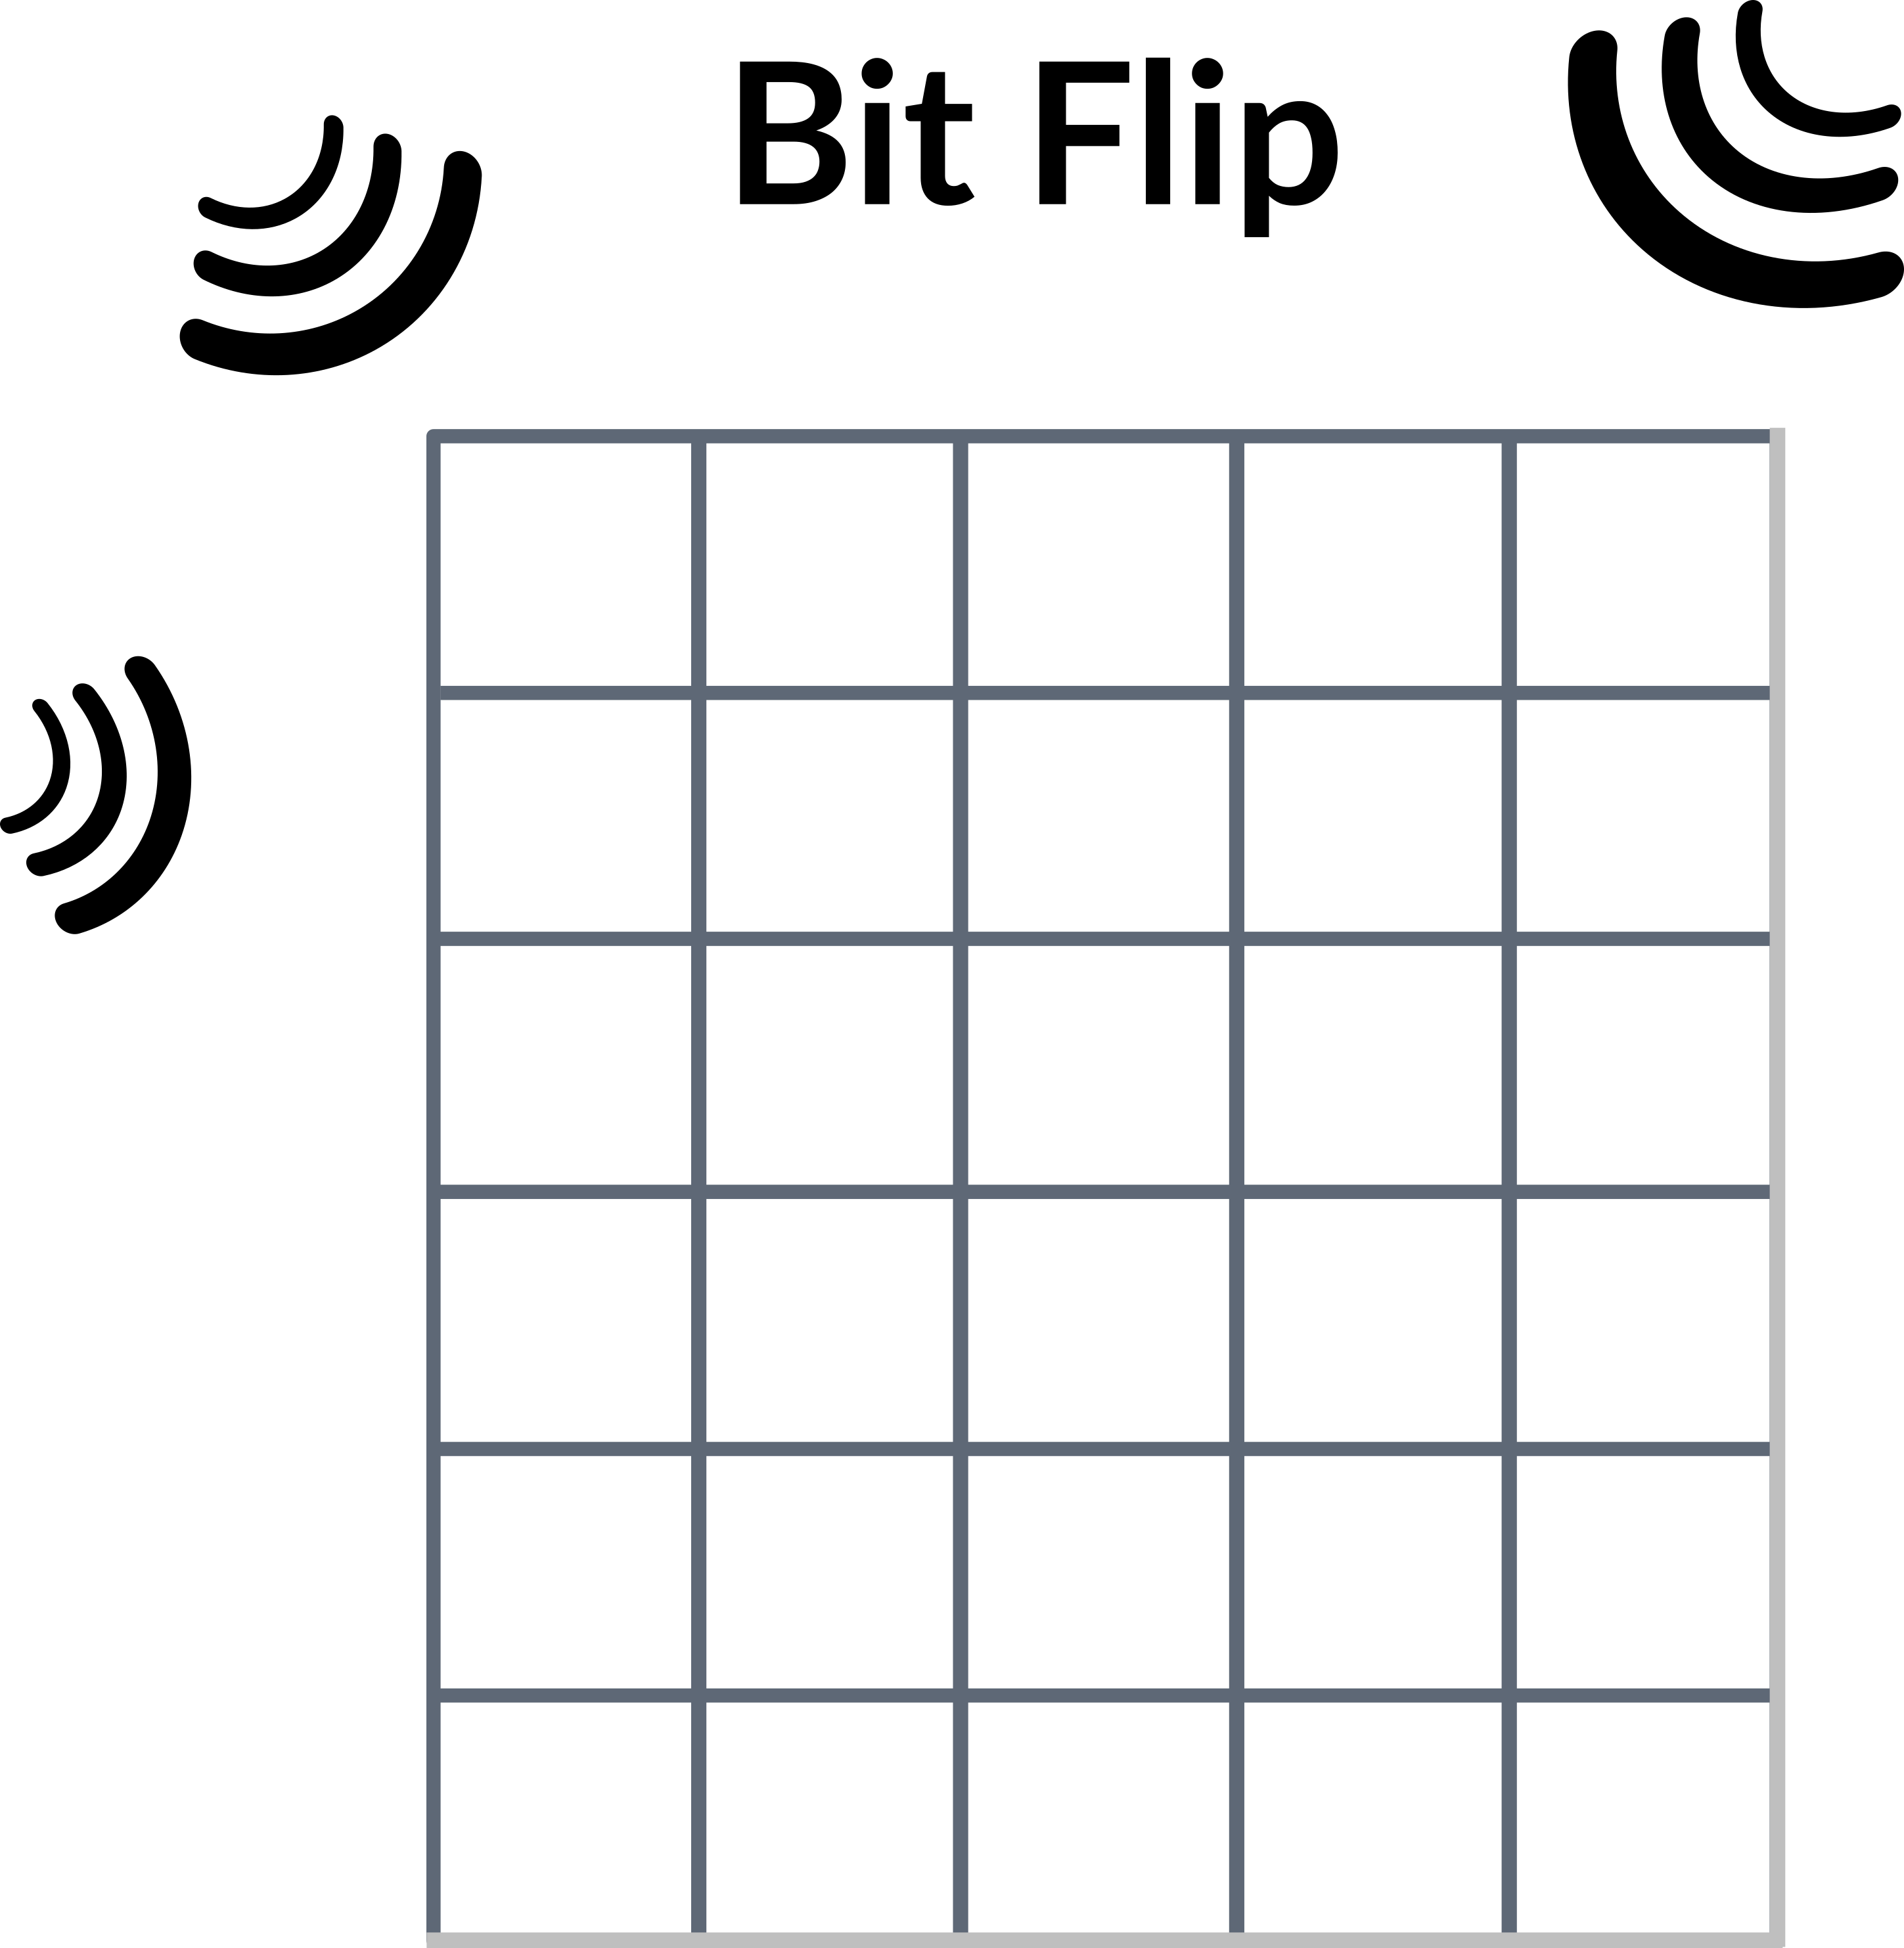
\includegraphics[width=0.4\textwidth]{fig/Toric_code_ex_1.png}
% 		\end{textblock*}
% 	}
% 	\only<2-2>{
% 		\begin{textblock*}{16cm}(4cm,1.7cm)
% 			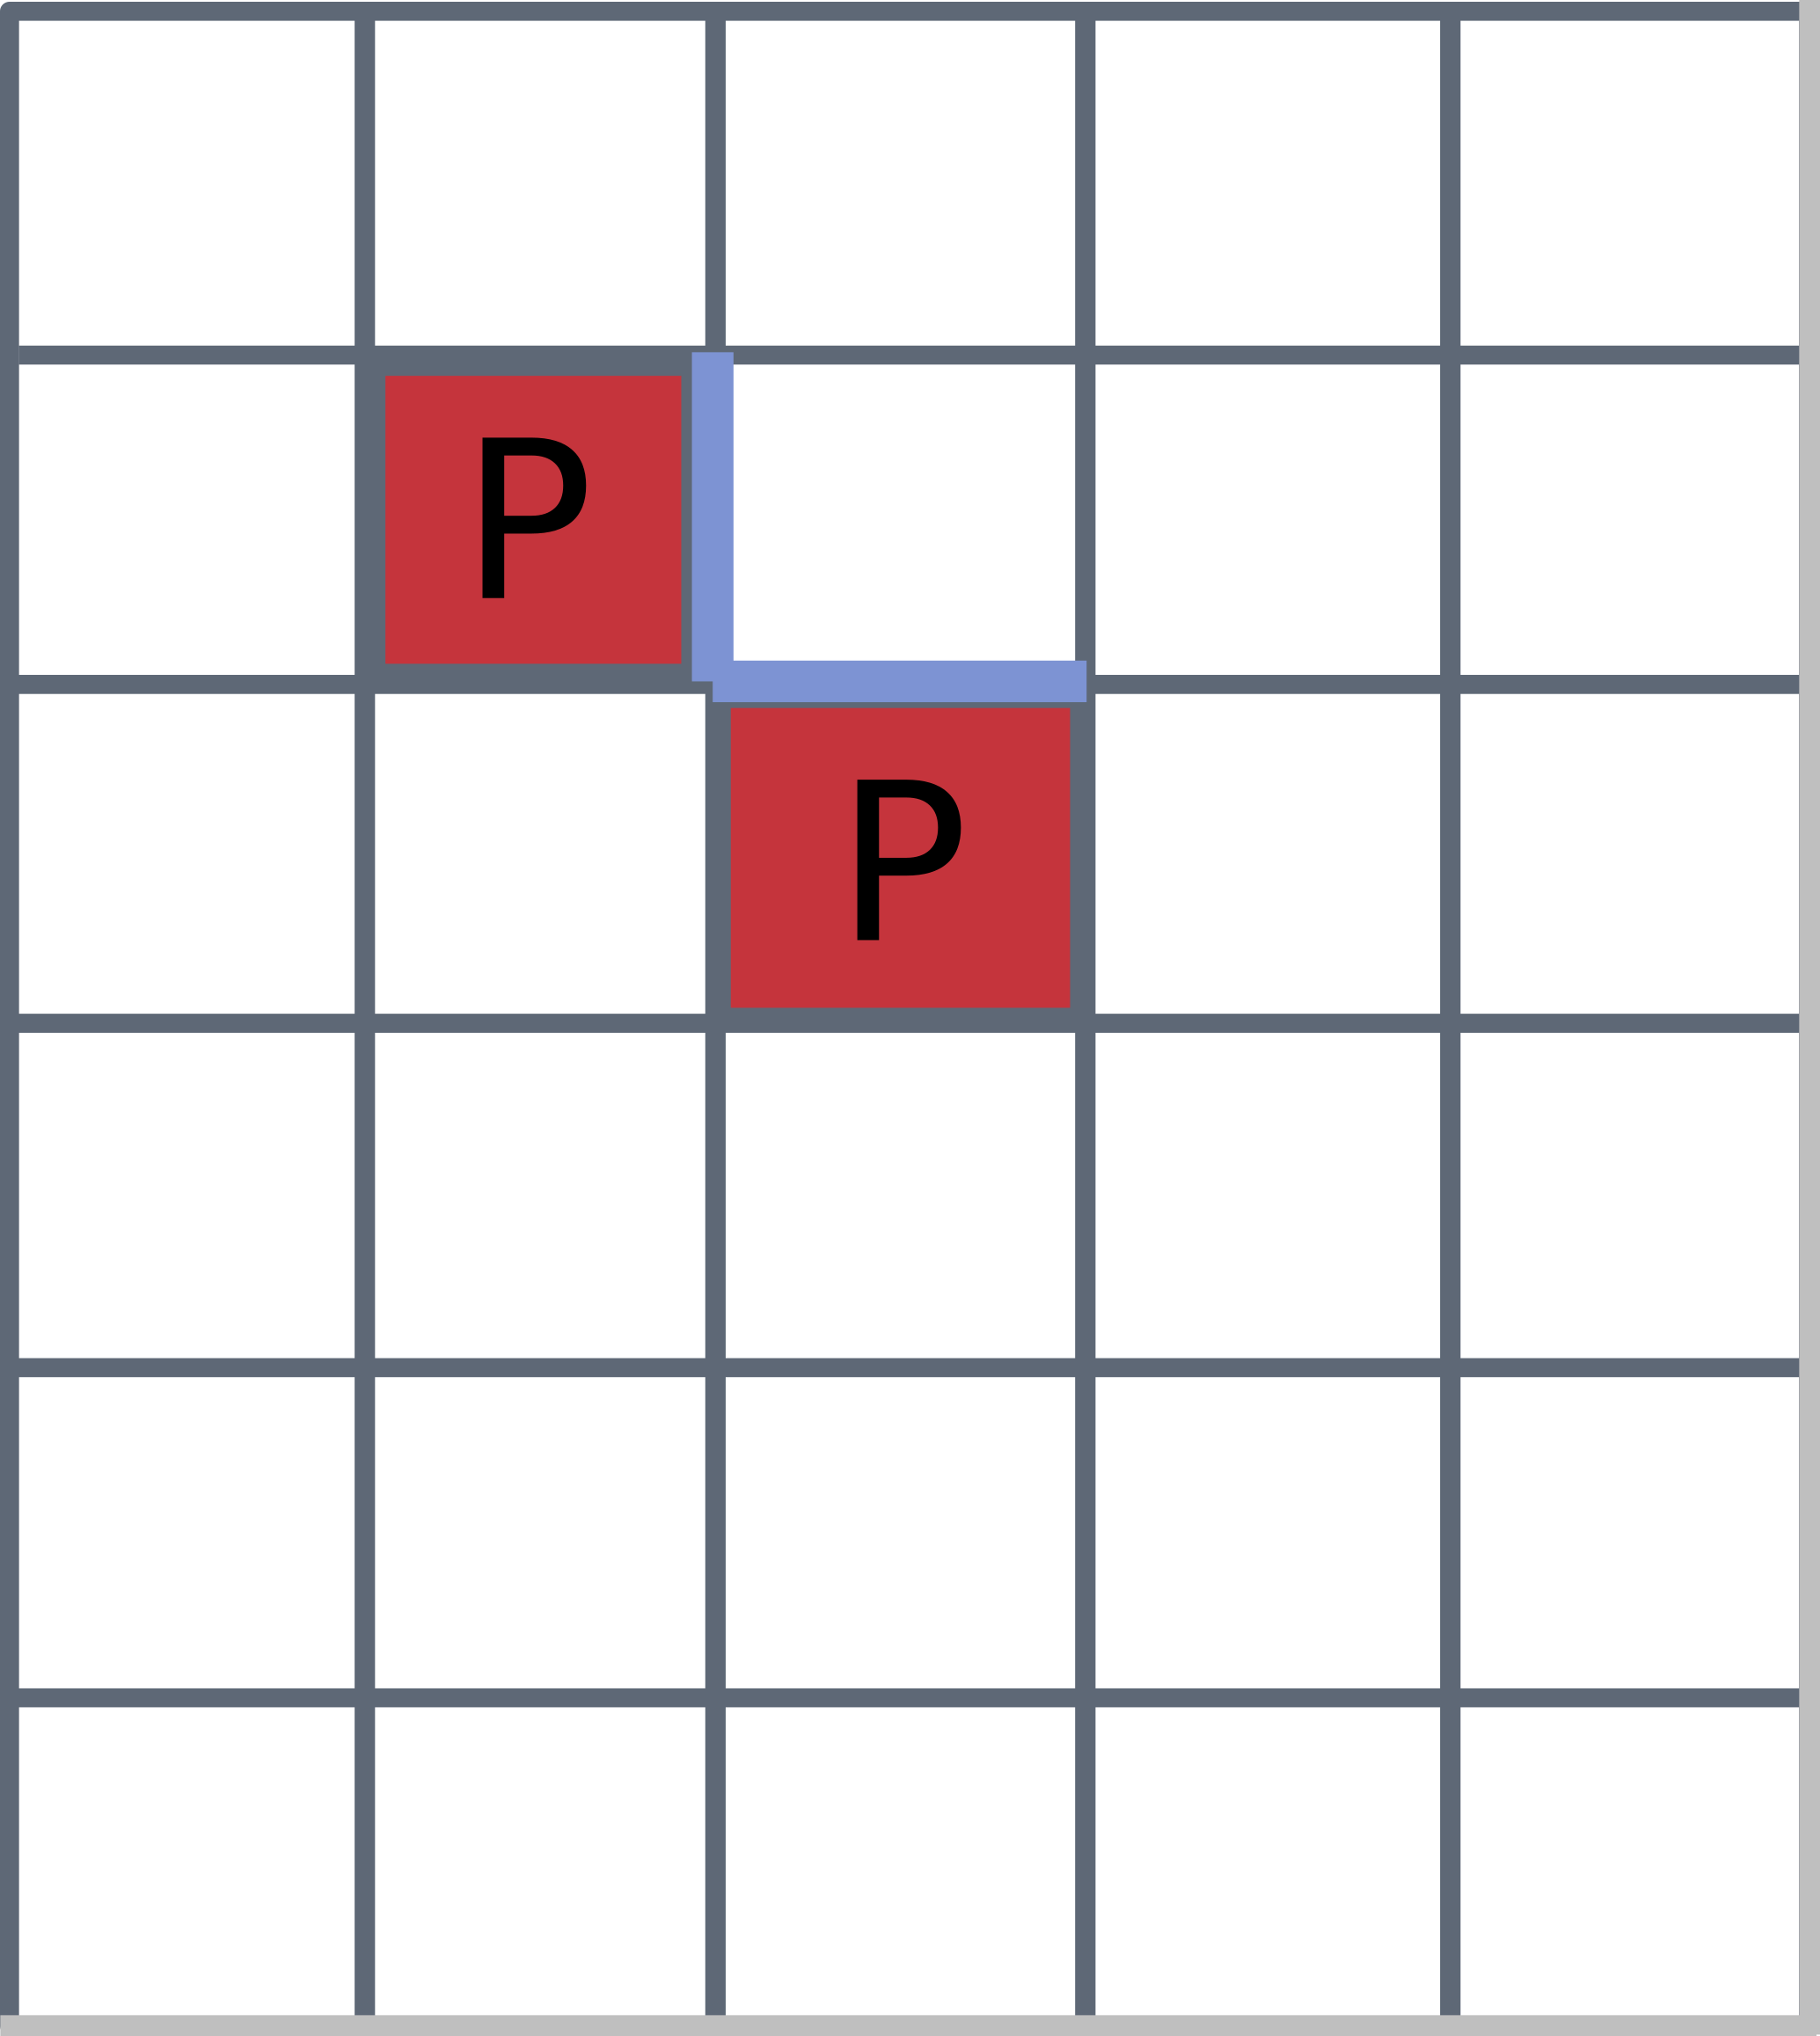
\includegraphics[width=0.35\textwidth]{fig/Toric_code_ex_2.png}
% 		\end{textblock*}
% 	}
% 	\only<3-3>{
% 		\begin{textblock*}{16cm}(2cm,1.7cm)
% 			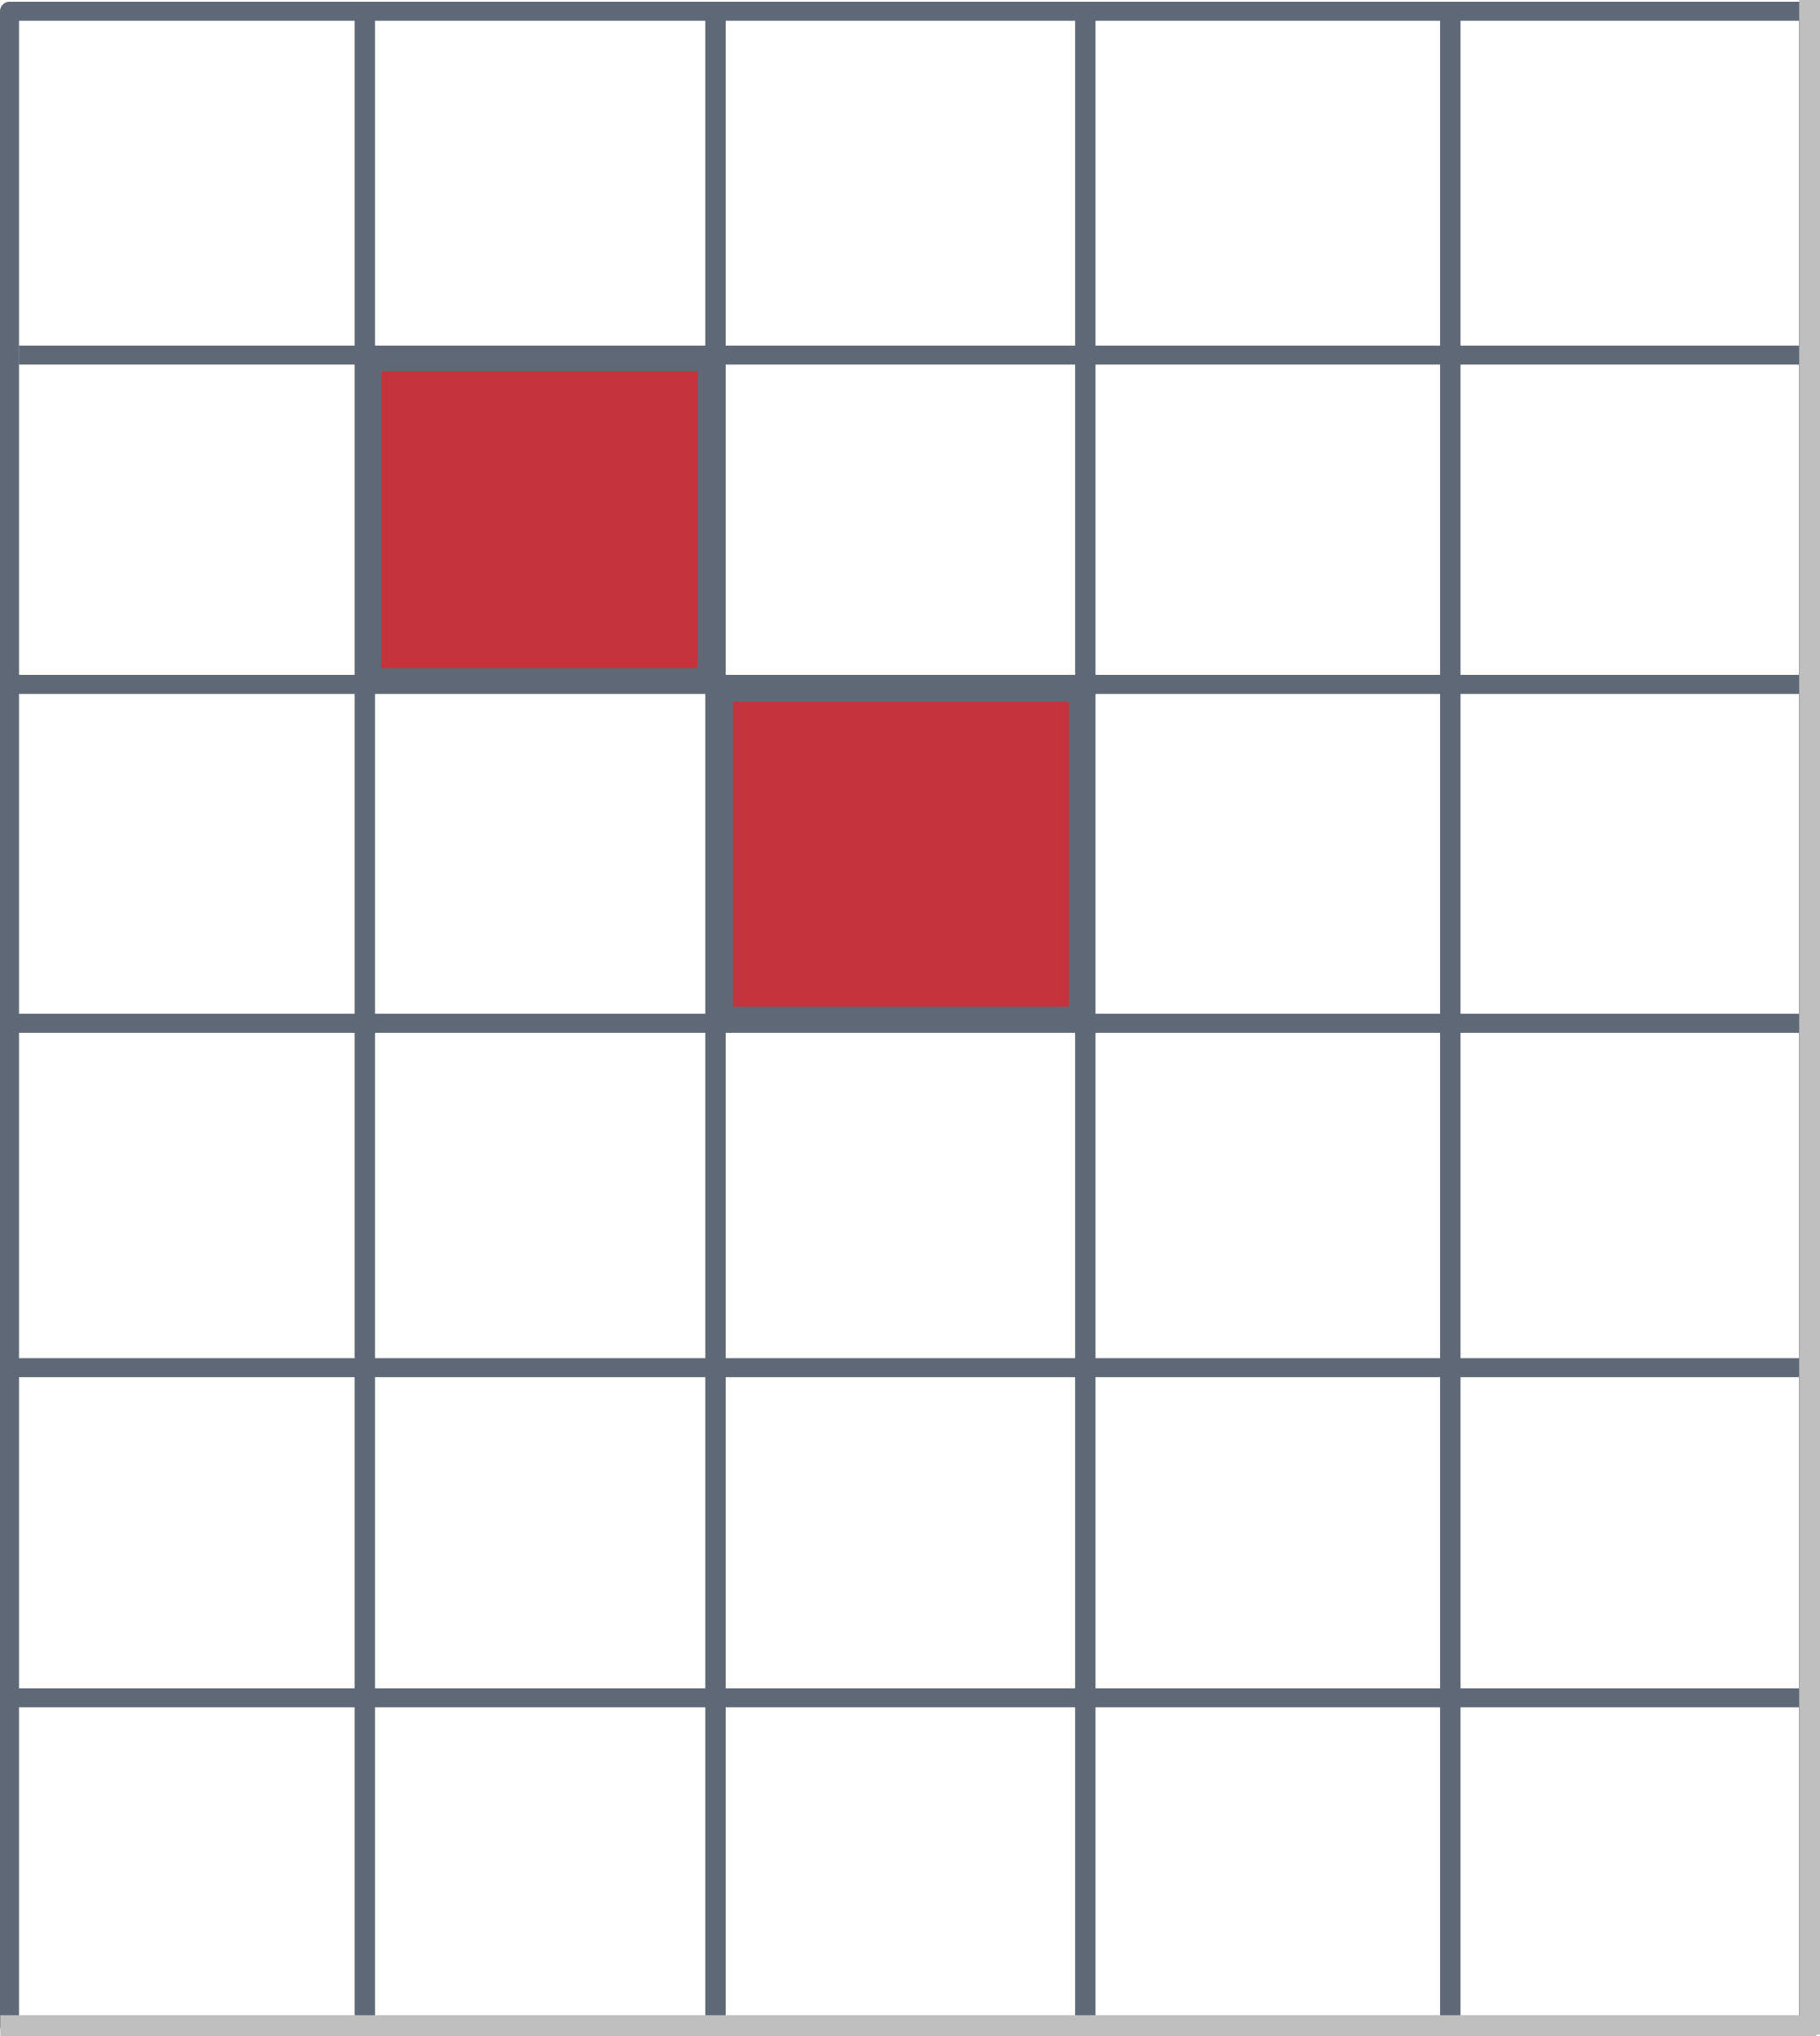
\includegraphics[width=0.35\textwidth]{fig/Toric_code_ex_3.png}
% 		\end{textblock*}
% 		\begin{textblock*}{7.5cm}(8cm,2cm)
% 			\textbf{Maximum probability (MP) decoding}\\
% 			\vspace{0.5cm}
% 			% $E_{\text{correction}}=\text{argmax}_{E\in \bar{\mathcal{G}}_{n}}P(E|s)$
% 			Select most probable physical error consistent with the partial error information
% 		\end{textblock*}
% 	}
% 	\only<4-4>{
% 		\begin{textblock*}{16cm}(2cm,1.7cm)
% 			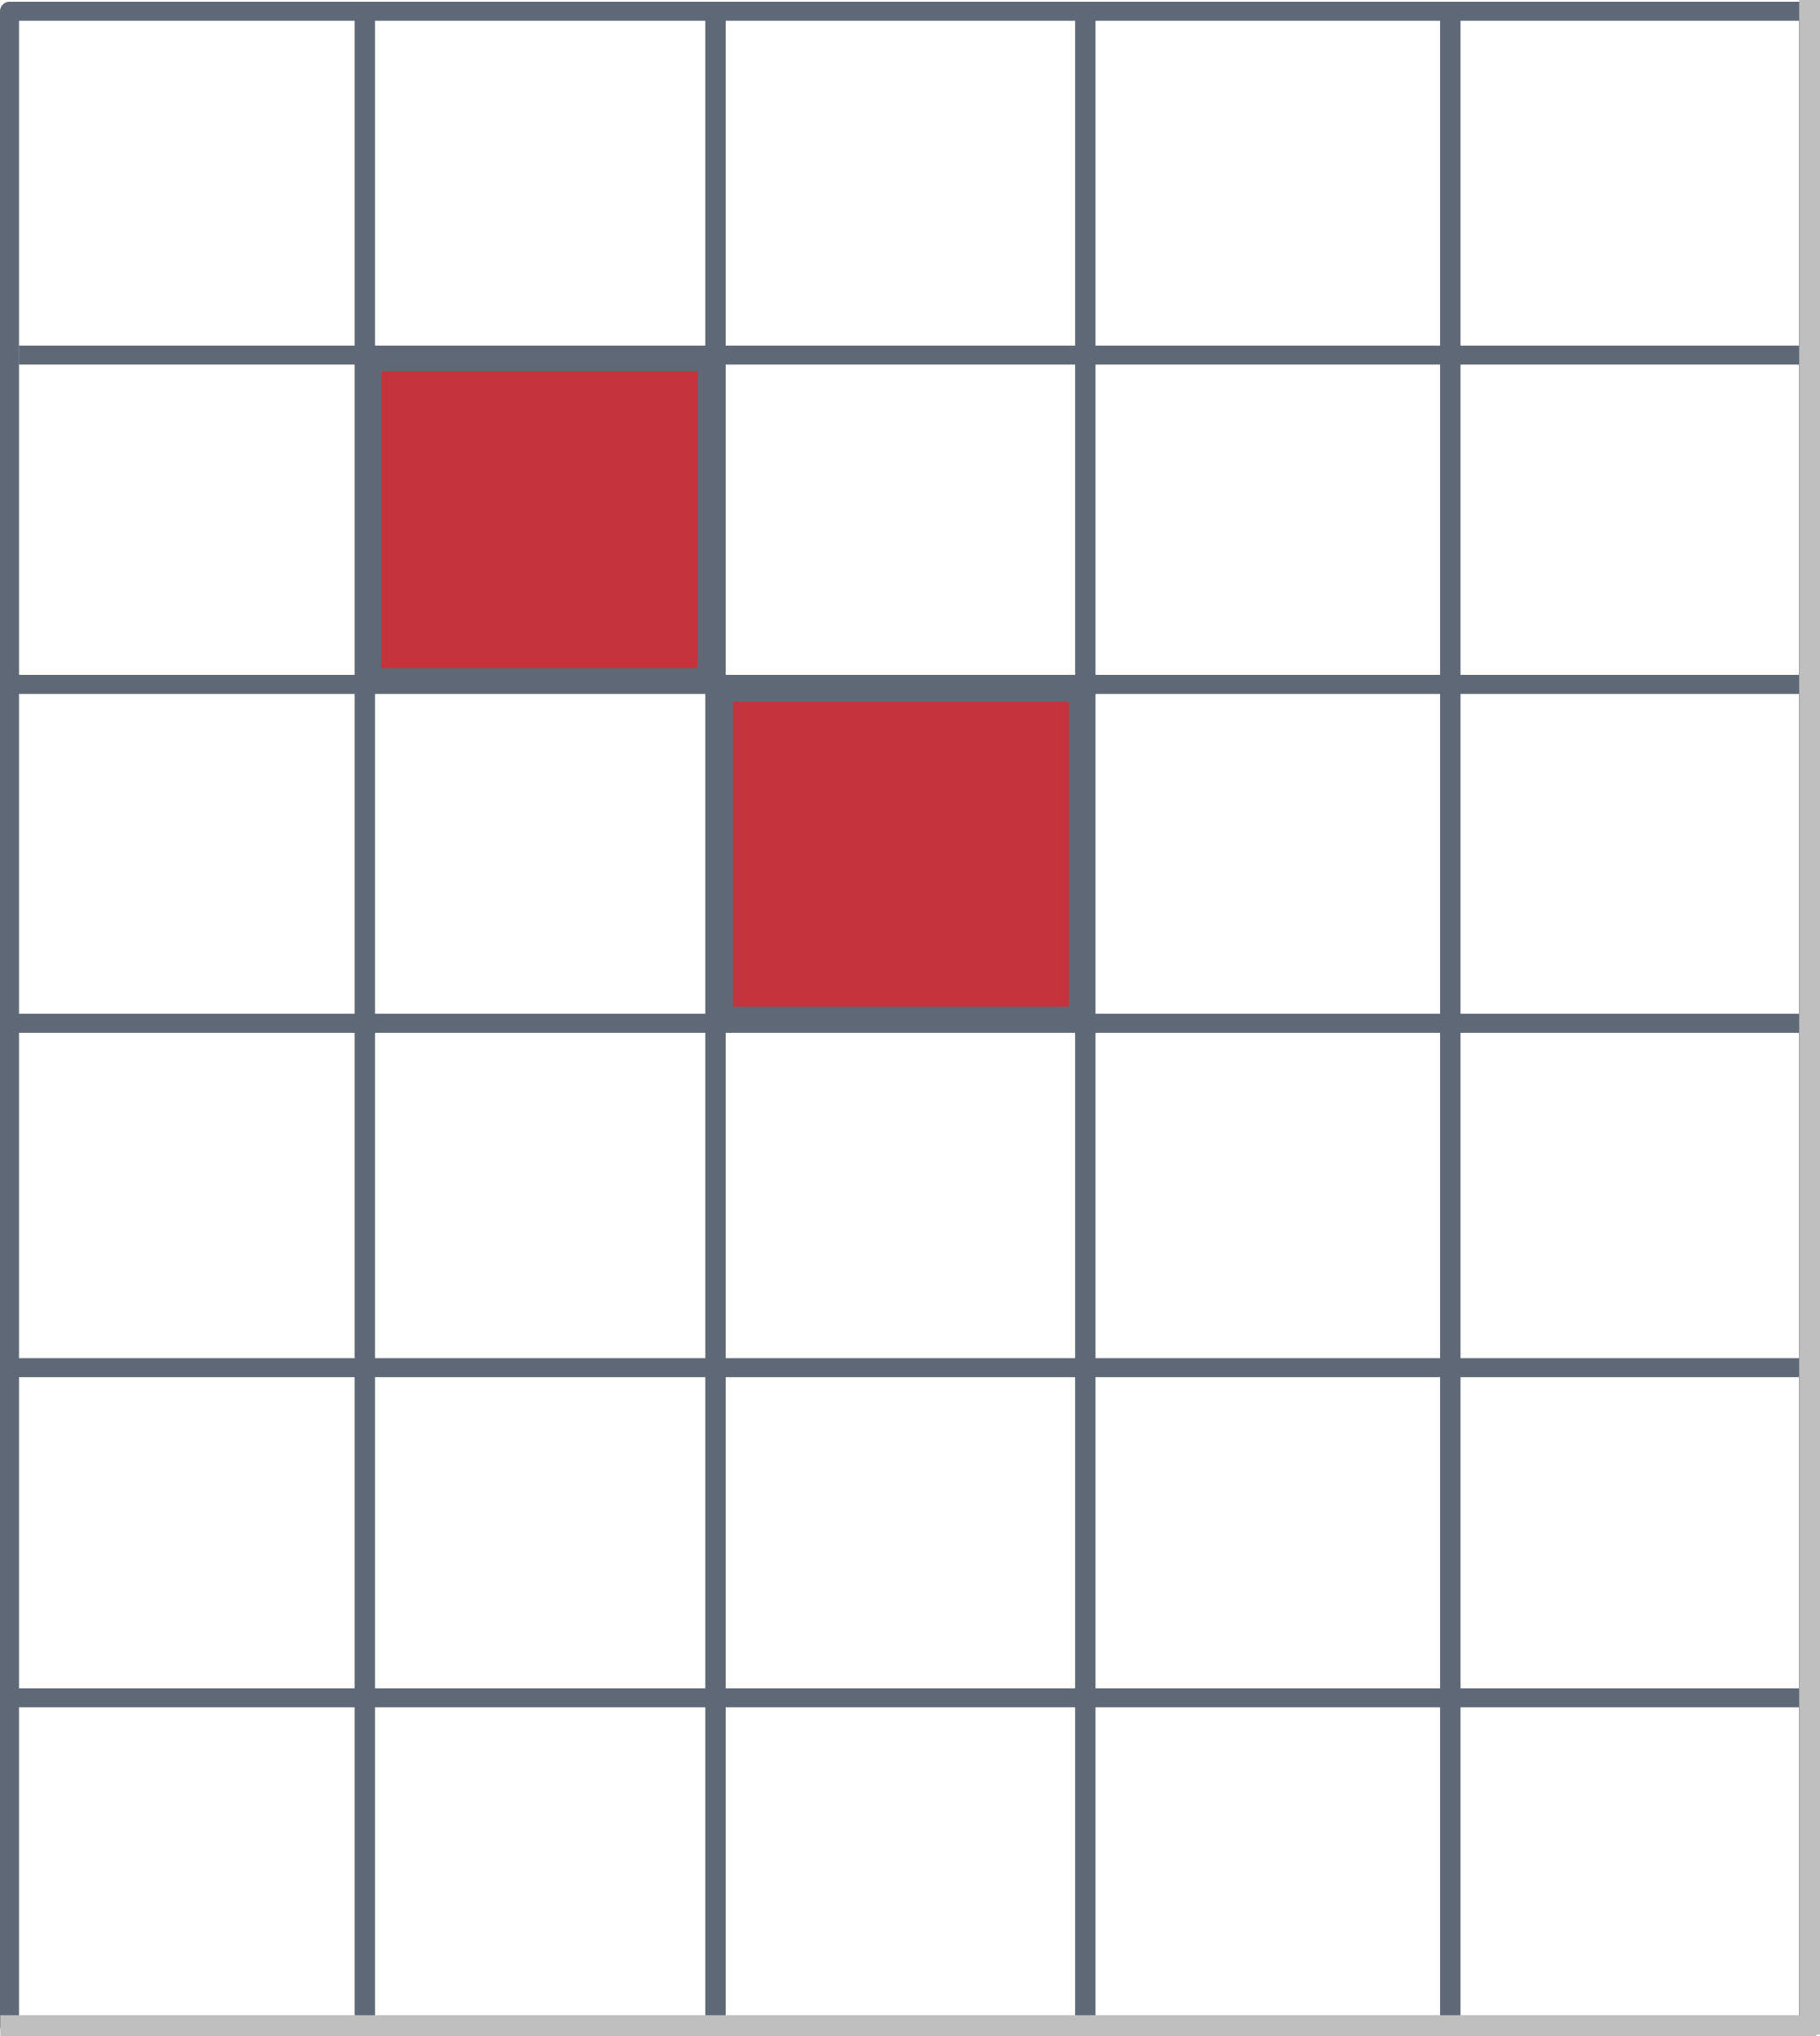
\includegraphics[width=0.35\textwidth]{fig/Toric_code_ex_3.png}
% 		\end{textblock*}
% 		\begin{textblock*}{7.5cm}(8cm,2cm)
% 			\textbf{MP/MWPM decoding}\\
% 			\vspace{0.5cm}
% 			% $E_{\text{correction}}=\text{argmax}_{E\in \bar{\mathcal{G}}_{n}}P(E|s)$
% 			Select physical error which acts on lowest number of qubits non trivially and is consistent with the partial error information
% 	\end{textblock*}
% 	}
% 	\only<5-5>{
% 		\begin{textblock*}{16cm}(2cm,1.7cm)
% 			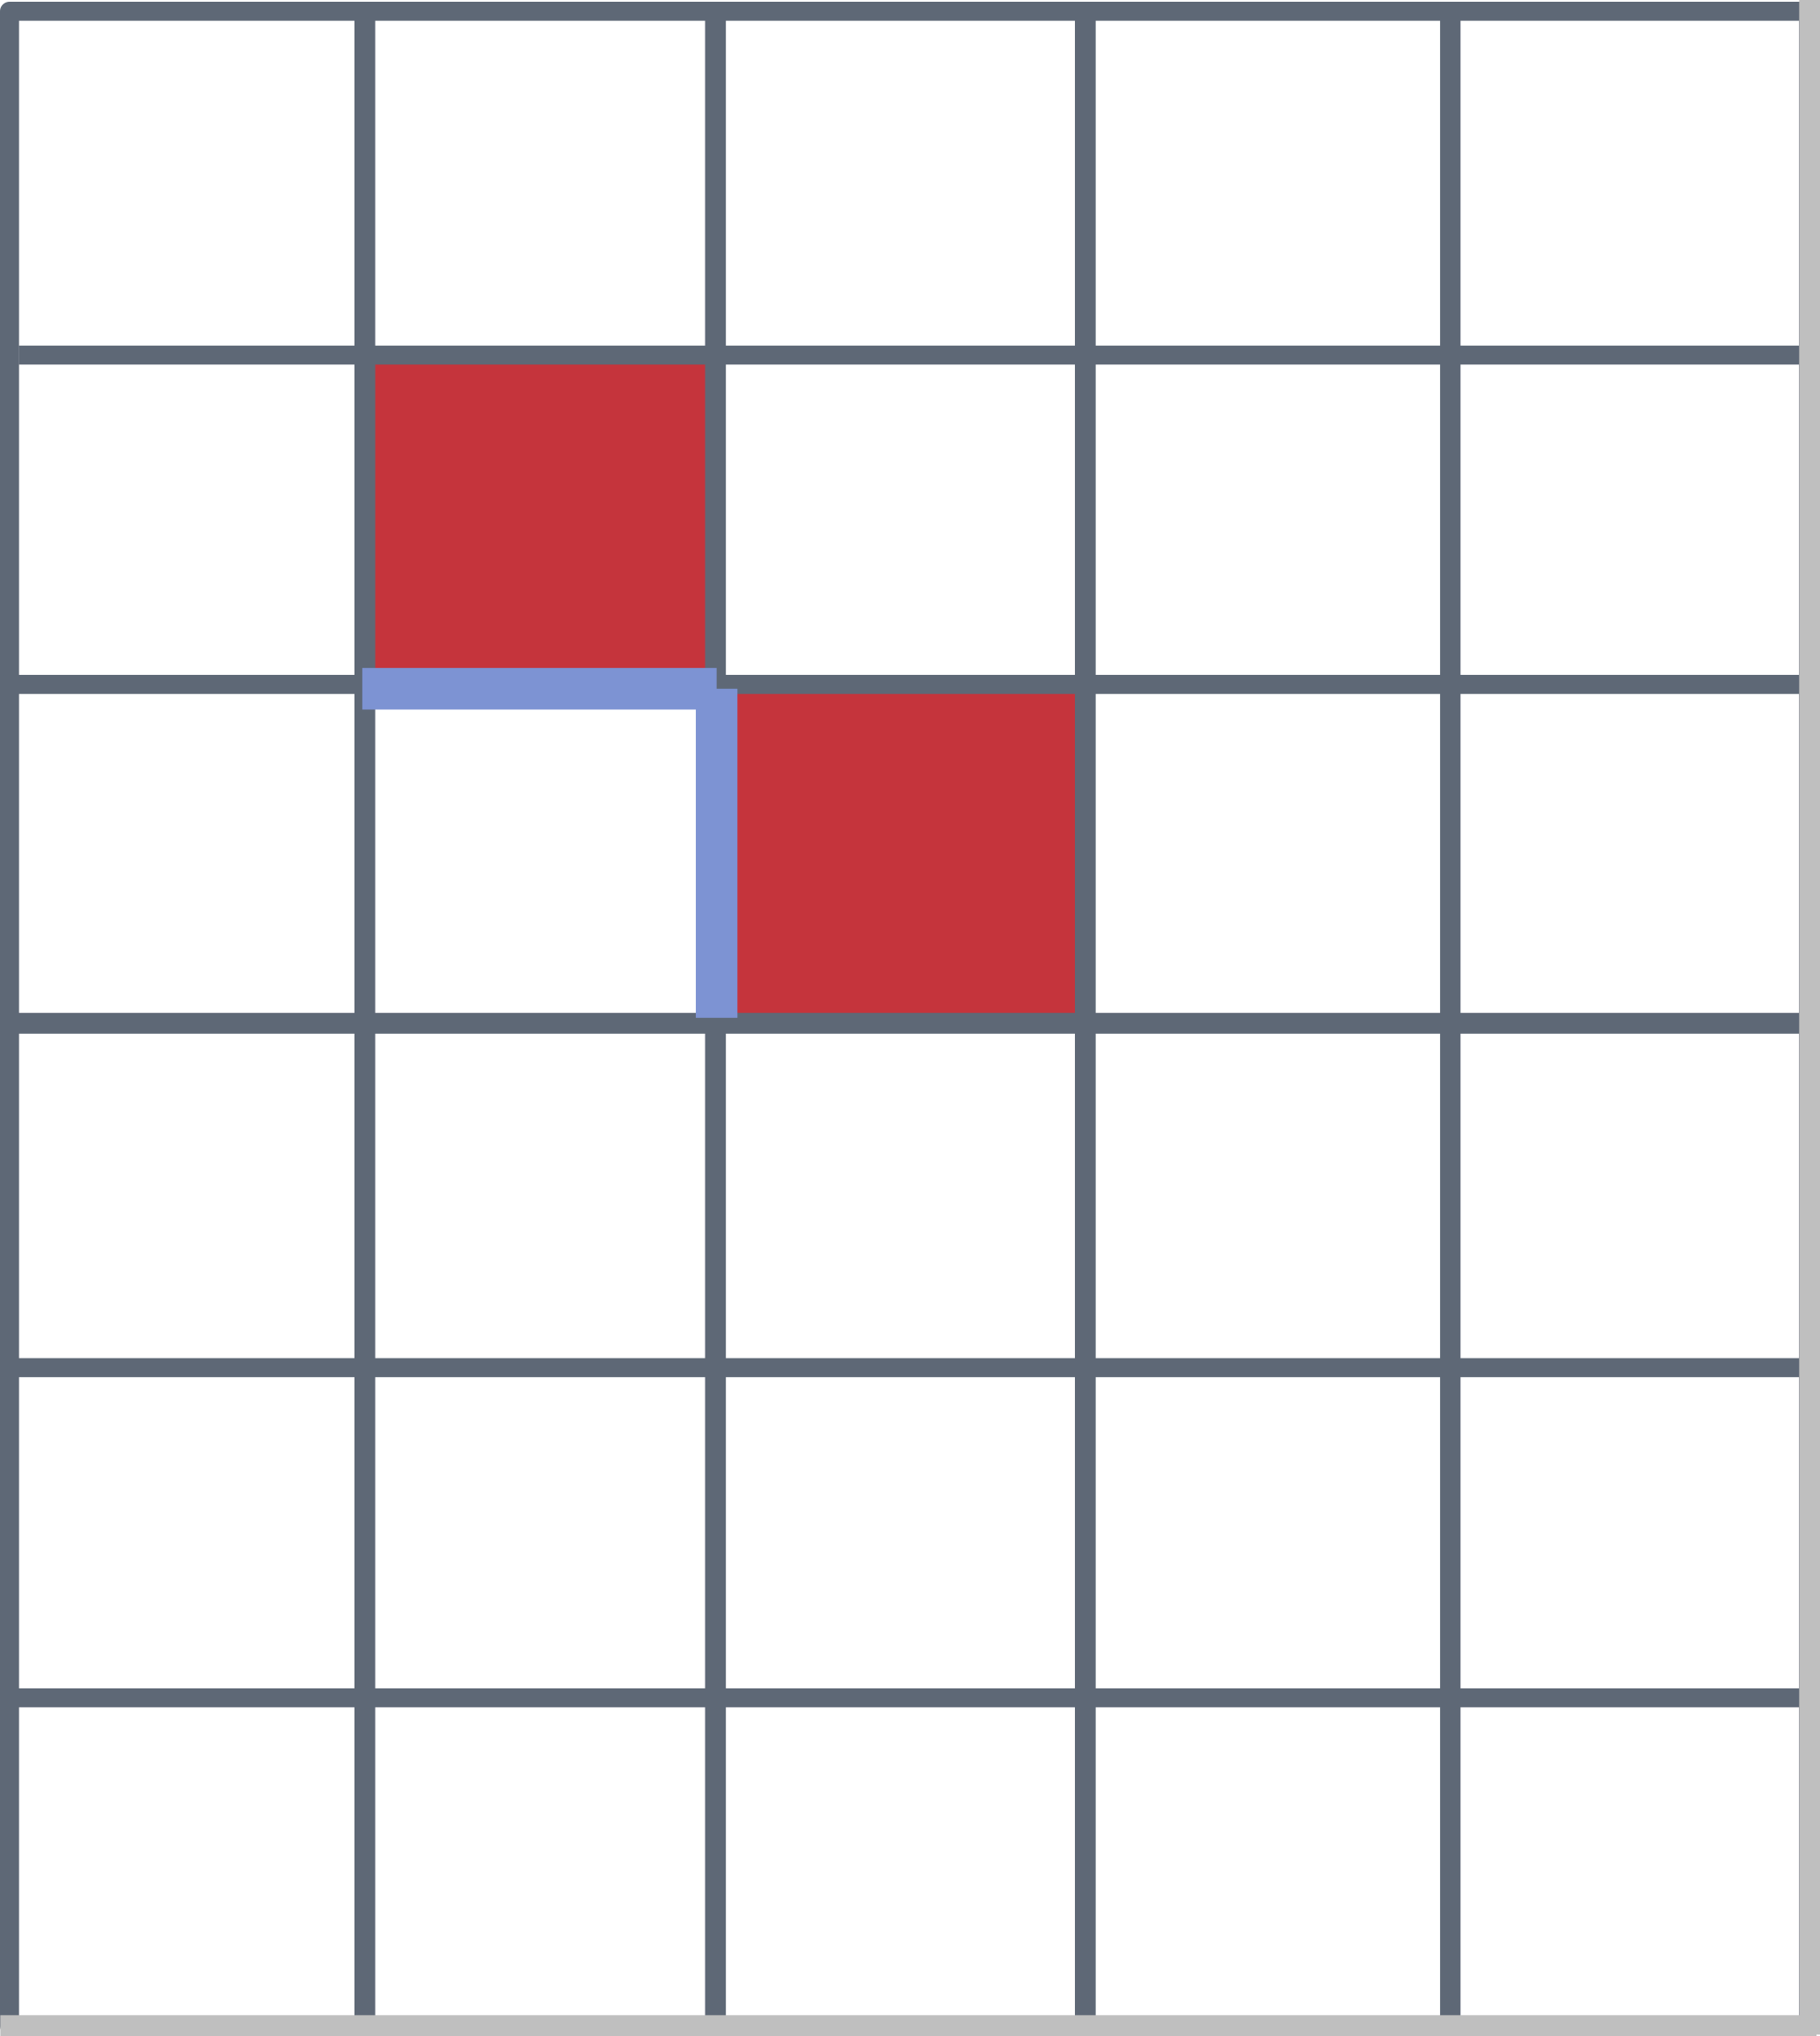
\includegraphics[width=0.35\textwidth]{fig/Toric_code_ex_6.png}
% 		\end{textblock*}
% 		\begin{textblock*}{7.5cm}(8cm,2cm)
% 			\textbf{MP/MWPM decoding}\\
% 			\vspace{0.5cm}
% 			% $E_{\text{correction}}=\text{argmax}_{E\in \bar{\mathcal{G}}_{n}}P(E|s)$
% 			Select physical error which acts on lowest number of qubits non trivially and is consistent with the partial error information
% 		\end{textblock*}
% 	}
% 	\only<6-6>{
% 		\begin{textblock*}{16cm}(2cm,1.7cm)
% 			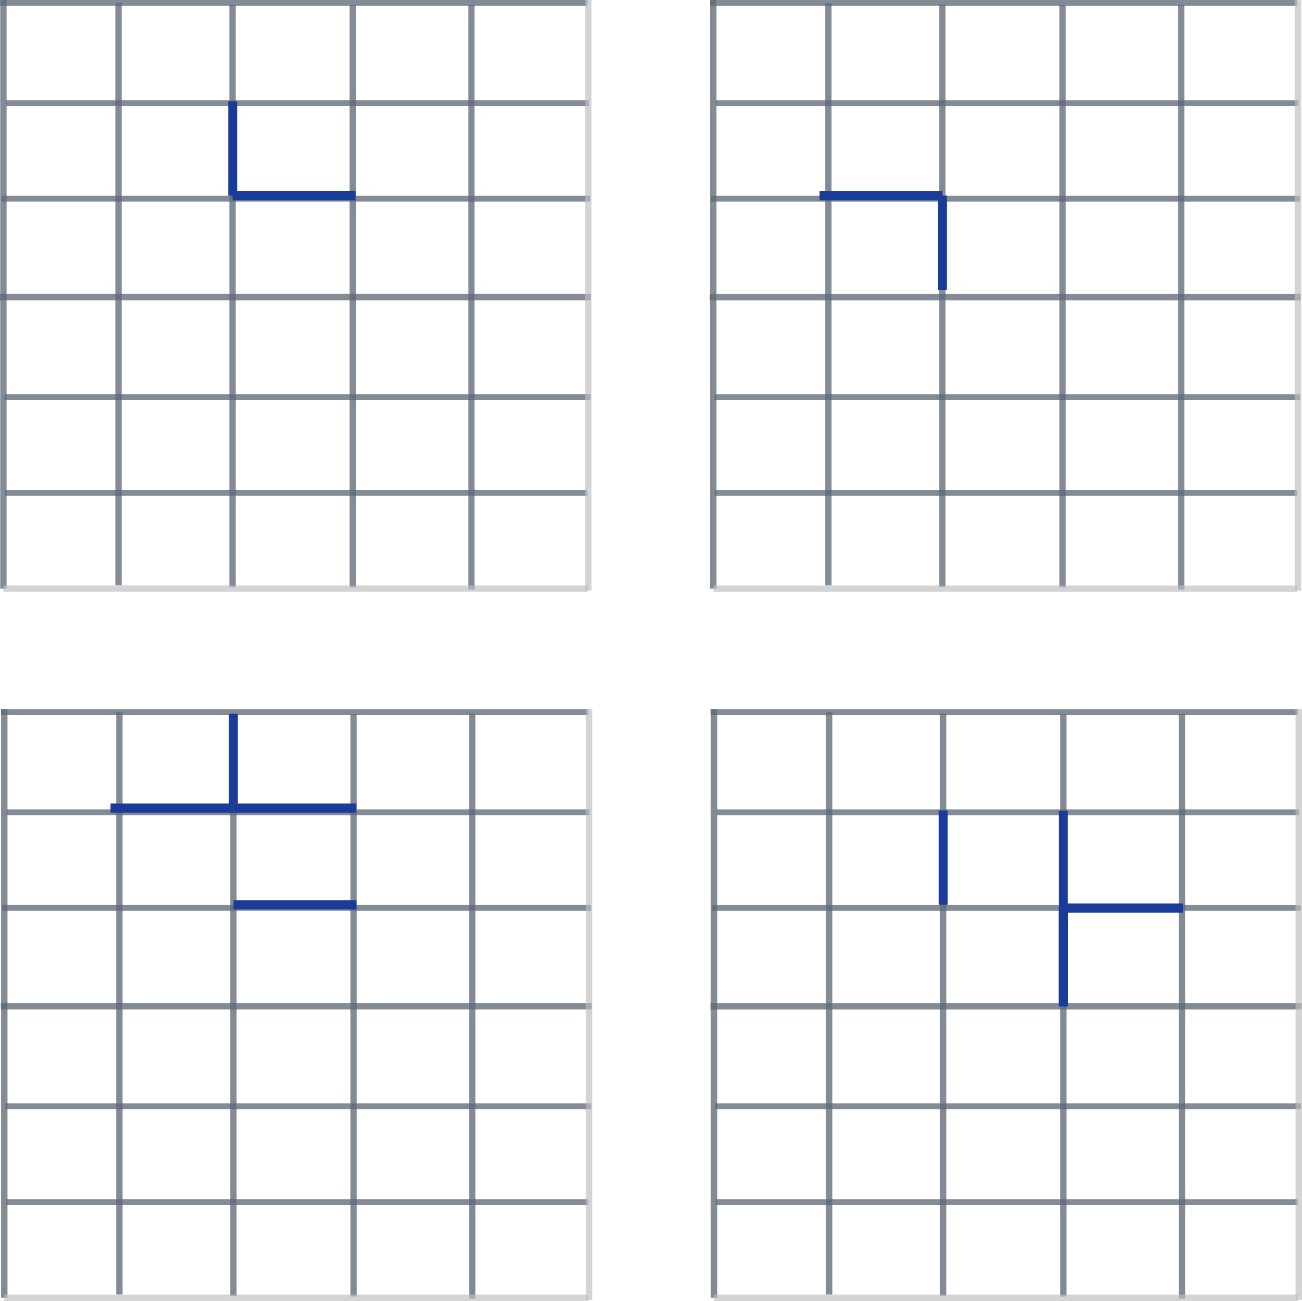
\includegraphics[width=0.35\textwidth]{fig/Toric_code_ex_9.png}
% 		\end{textblock*}
% 		\begin{textblock*}{8cm}(8cm,2cm)
% 			\textbf{Maximum likelihood/optimal decoding}\\
% 			Takes redundancy into account
% 		\end{textblock*}
% 	}
% 	\only<6-6>{
% 		\begin{textblock*}{16cm}(2cm,1.7cm)
% 			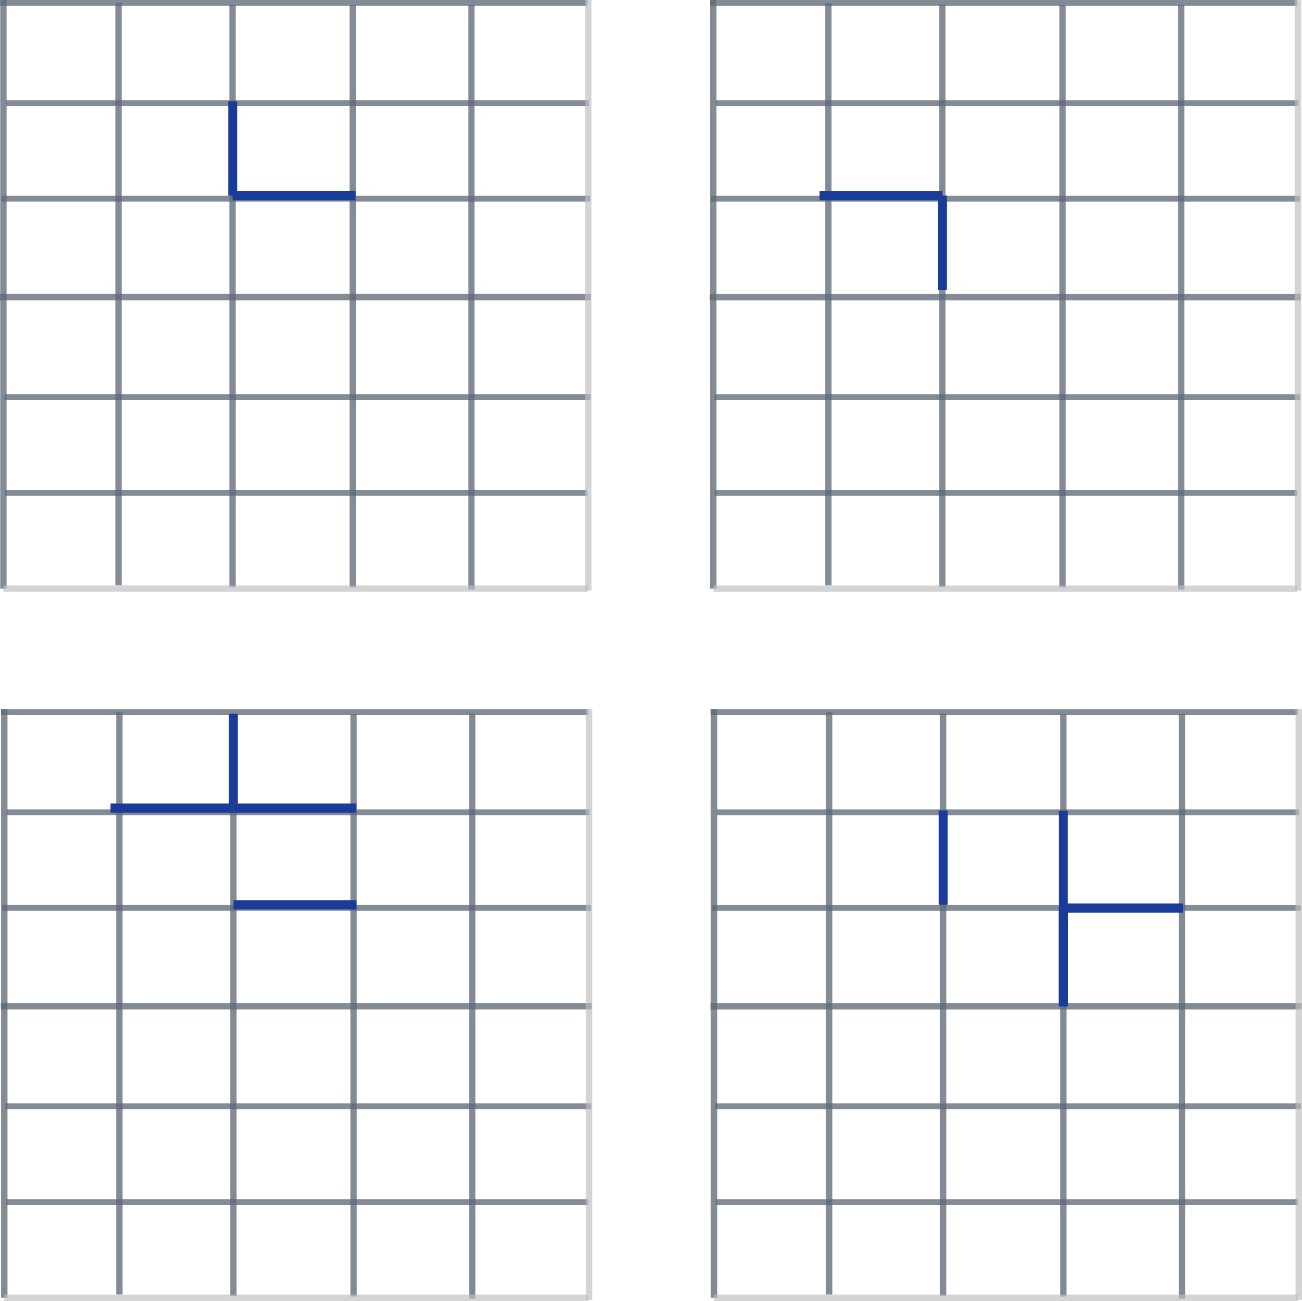
\includegraphics[width=0.35\textwidth]{fig/Toric_code_ex_9.png}
% 		\end{textblock*}
% 		\begin{textblock*}{8cm}(8cm,2cm)
% 			\textbf{Maximum likelihood/optimal decoding}\\
% 			Takes redundancy into account
% 		\end{textblock*}
% 	}
% 	% \only<6-6>{
% 	% \begin{textblock*}{16cm}(4cm,1.7cm)
% 	% 	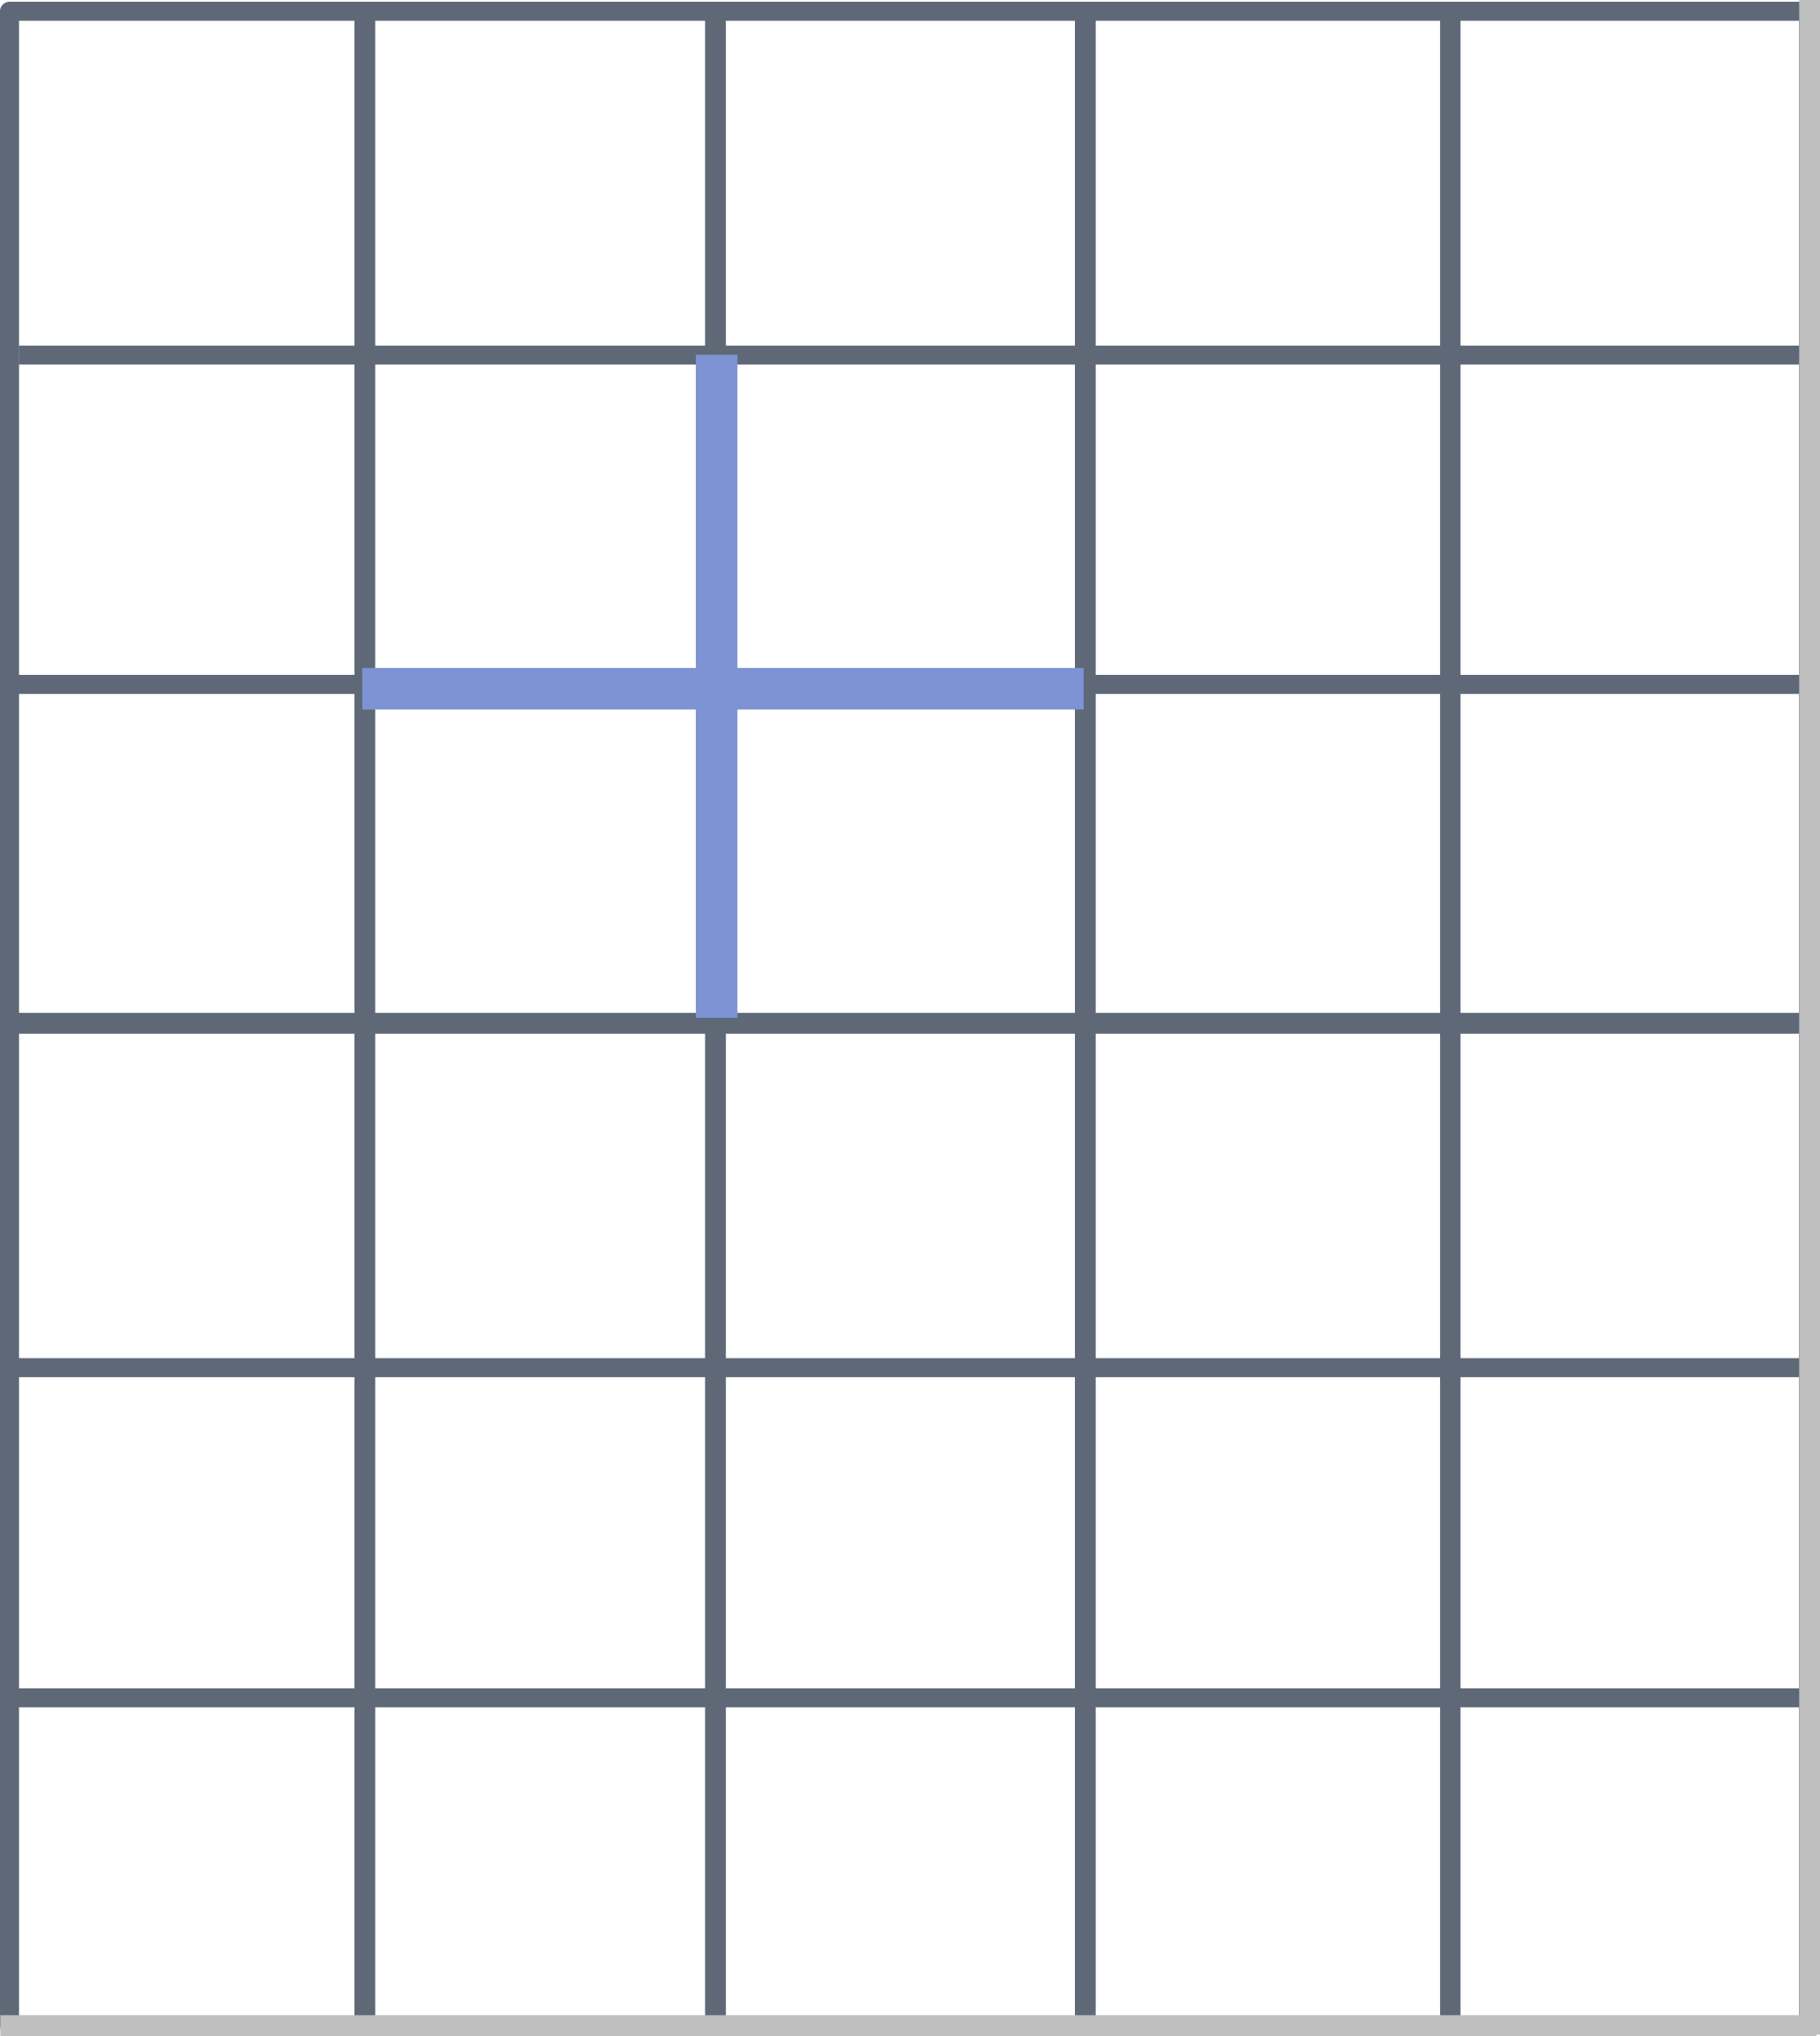
\includegraphics[width=0.35\textwidth]{fig/Toric_code_ex_7.png}
% 	% \end{textblock*}
% 	% \begin{textblock*}{6cm}(10cm,2cm)
% 	% 	\textbf{success!} \\ But didnt take degeneracy into account
% 	% \end{textblock*}
% 	% }
% 	% \only<7-7>{
% 	% \begin{textblock*}{16cm}(2cm,1.7cm)
% 	% 	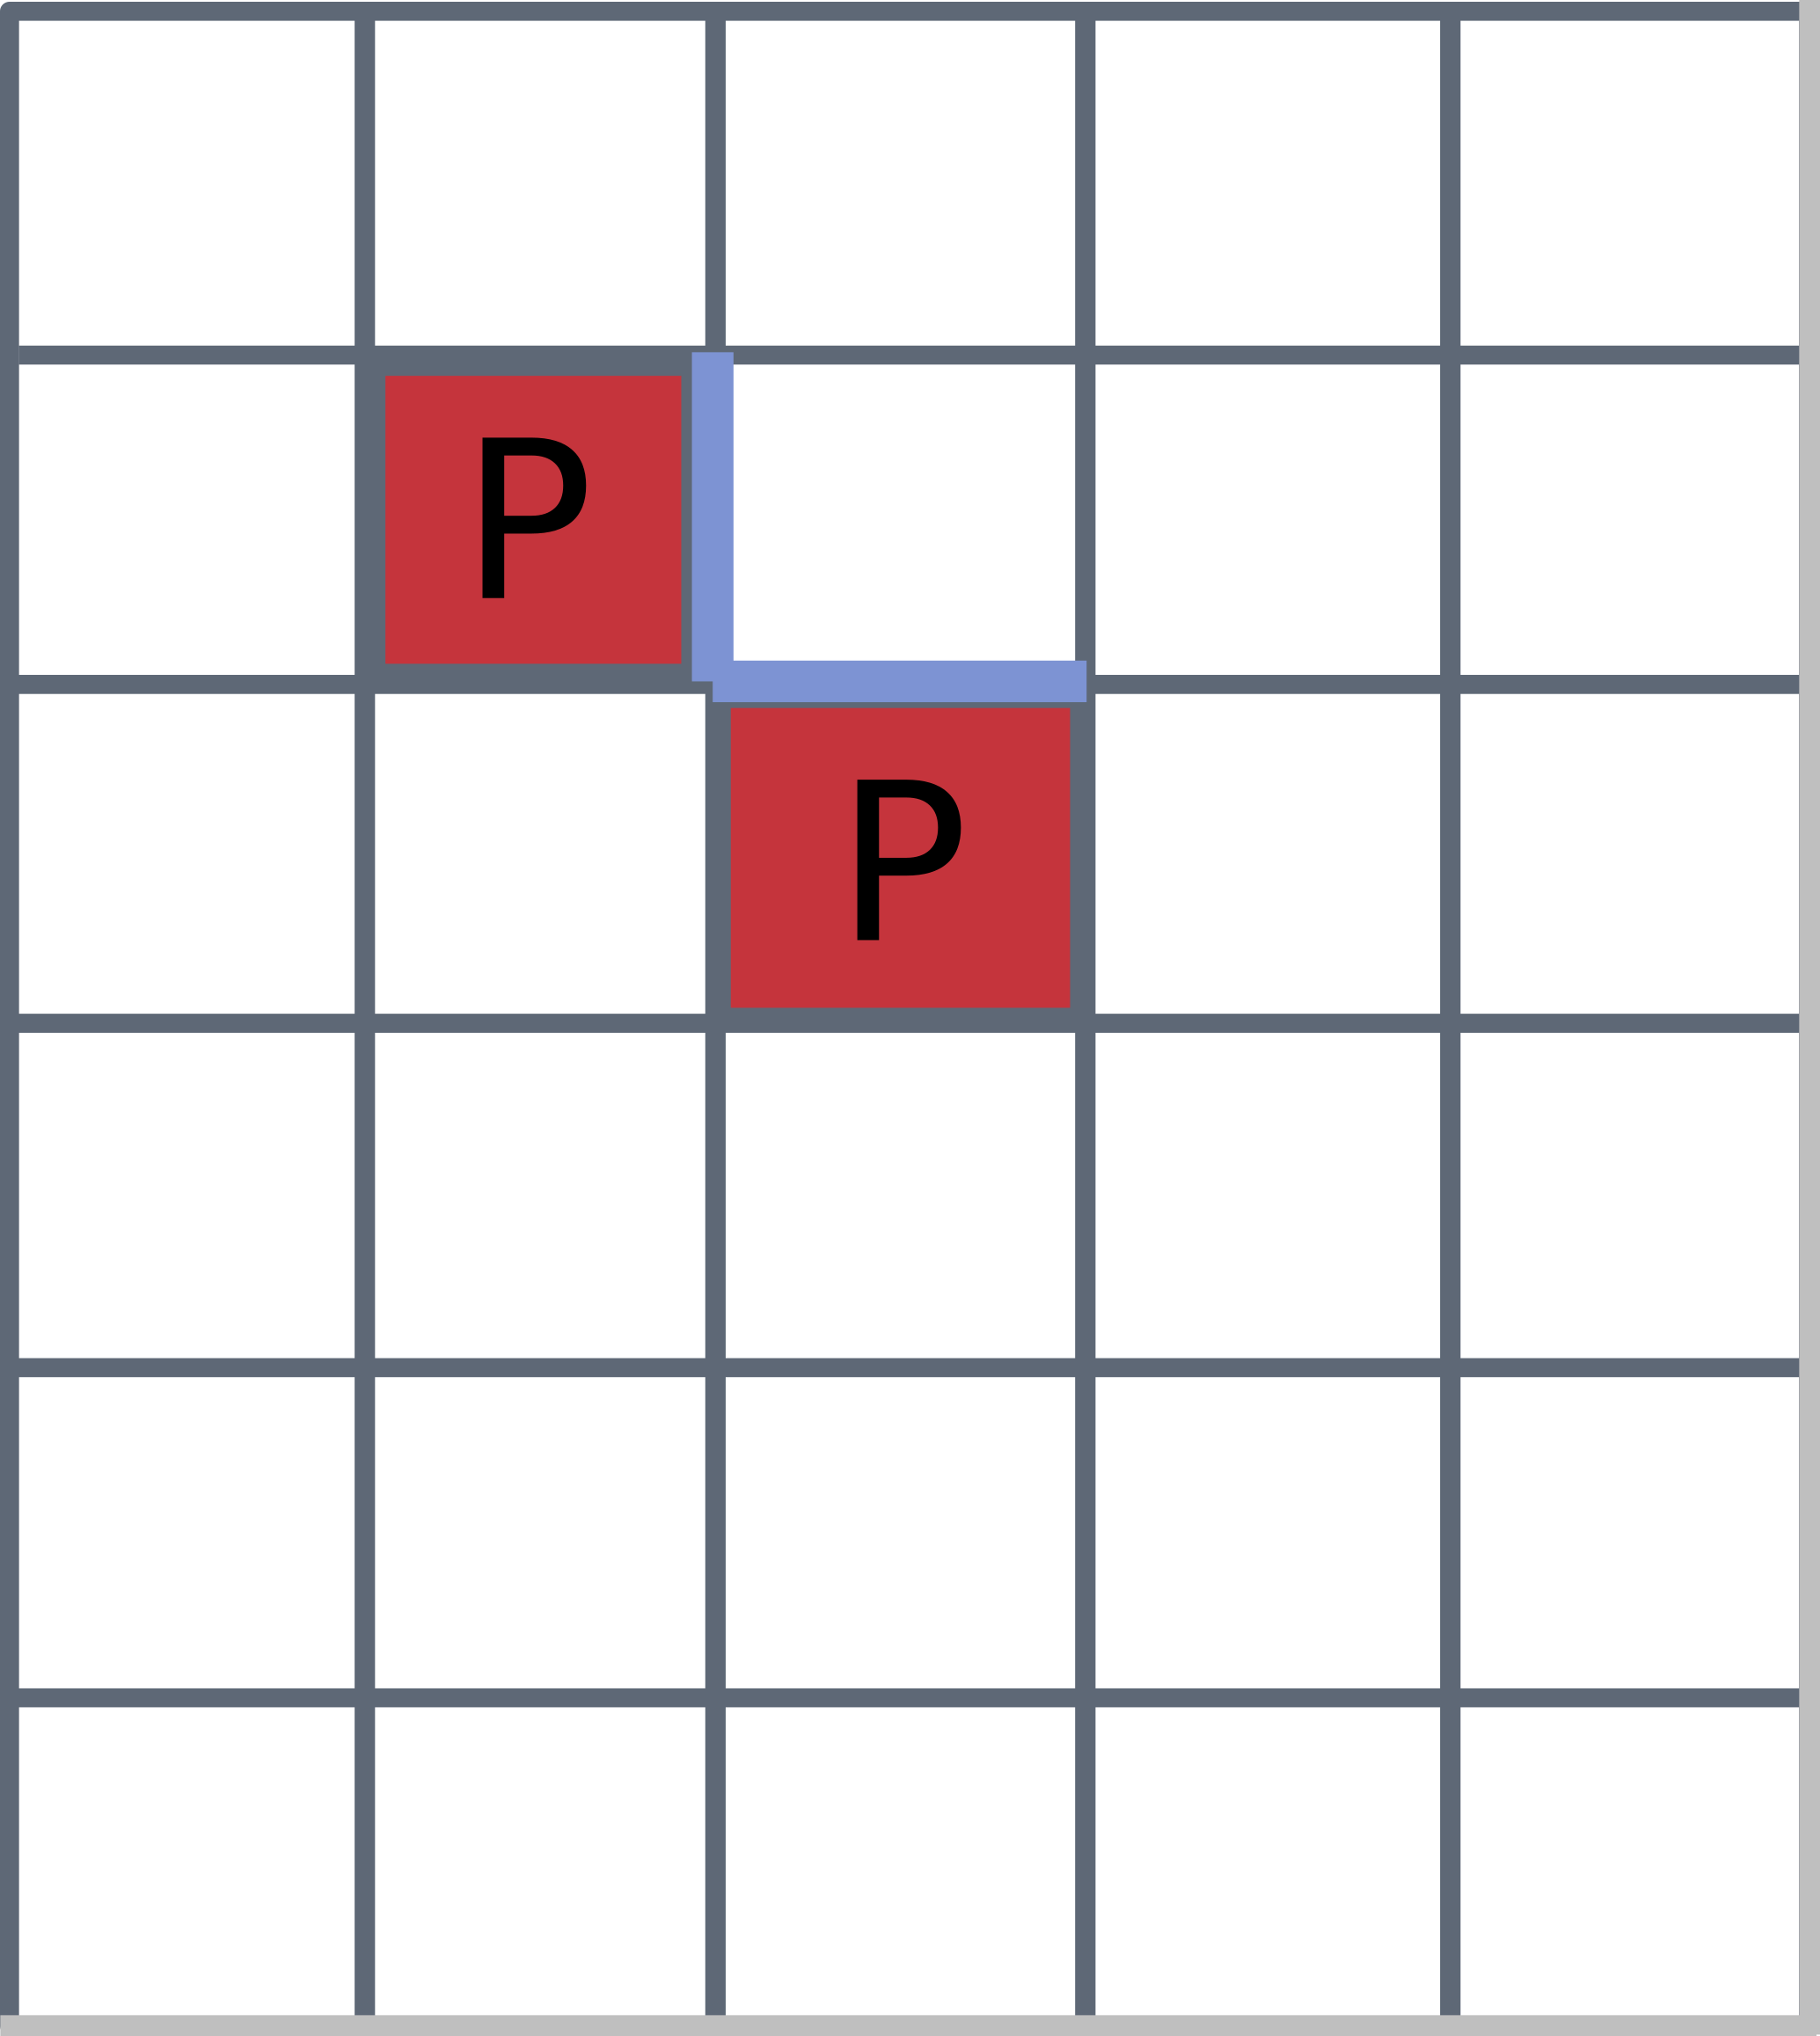
\includegraphics[width=0.35\textwidth]{fig/Toric_code_ex_2.png}
% 	% \end{textblock*}
% 	% \begin{textblock*}{8cm}(8cm,2cm)
% 	% 	\textbf{Maximum likelihood/optimal decoding}\\
% 	% 	$C_{s} \in \mathcal{G}_{n}$ compatible with $s$\\
% 	% 	$[C_{s}]=SC_{s}$ \\
% 	% 	$s \mapsto C_{s}L_{\delta(s)}$ with \\
% 	% 	$\delta(s) = \arg\max_{l\in L}P([C_{s}L_{l}])$
% 	% \end{textblock*}
% 	% }
% 	\only<8-8>{
% 		\begin{textblock*}{16cm}(2cm,1.7cm)
% 			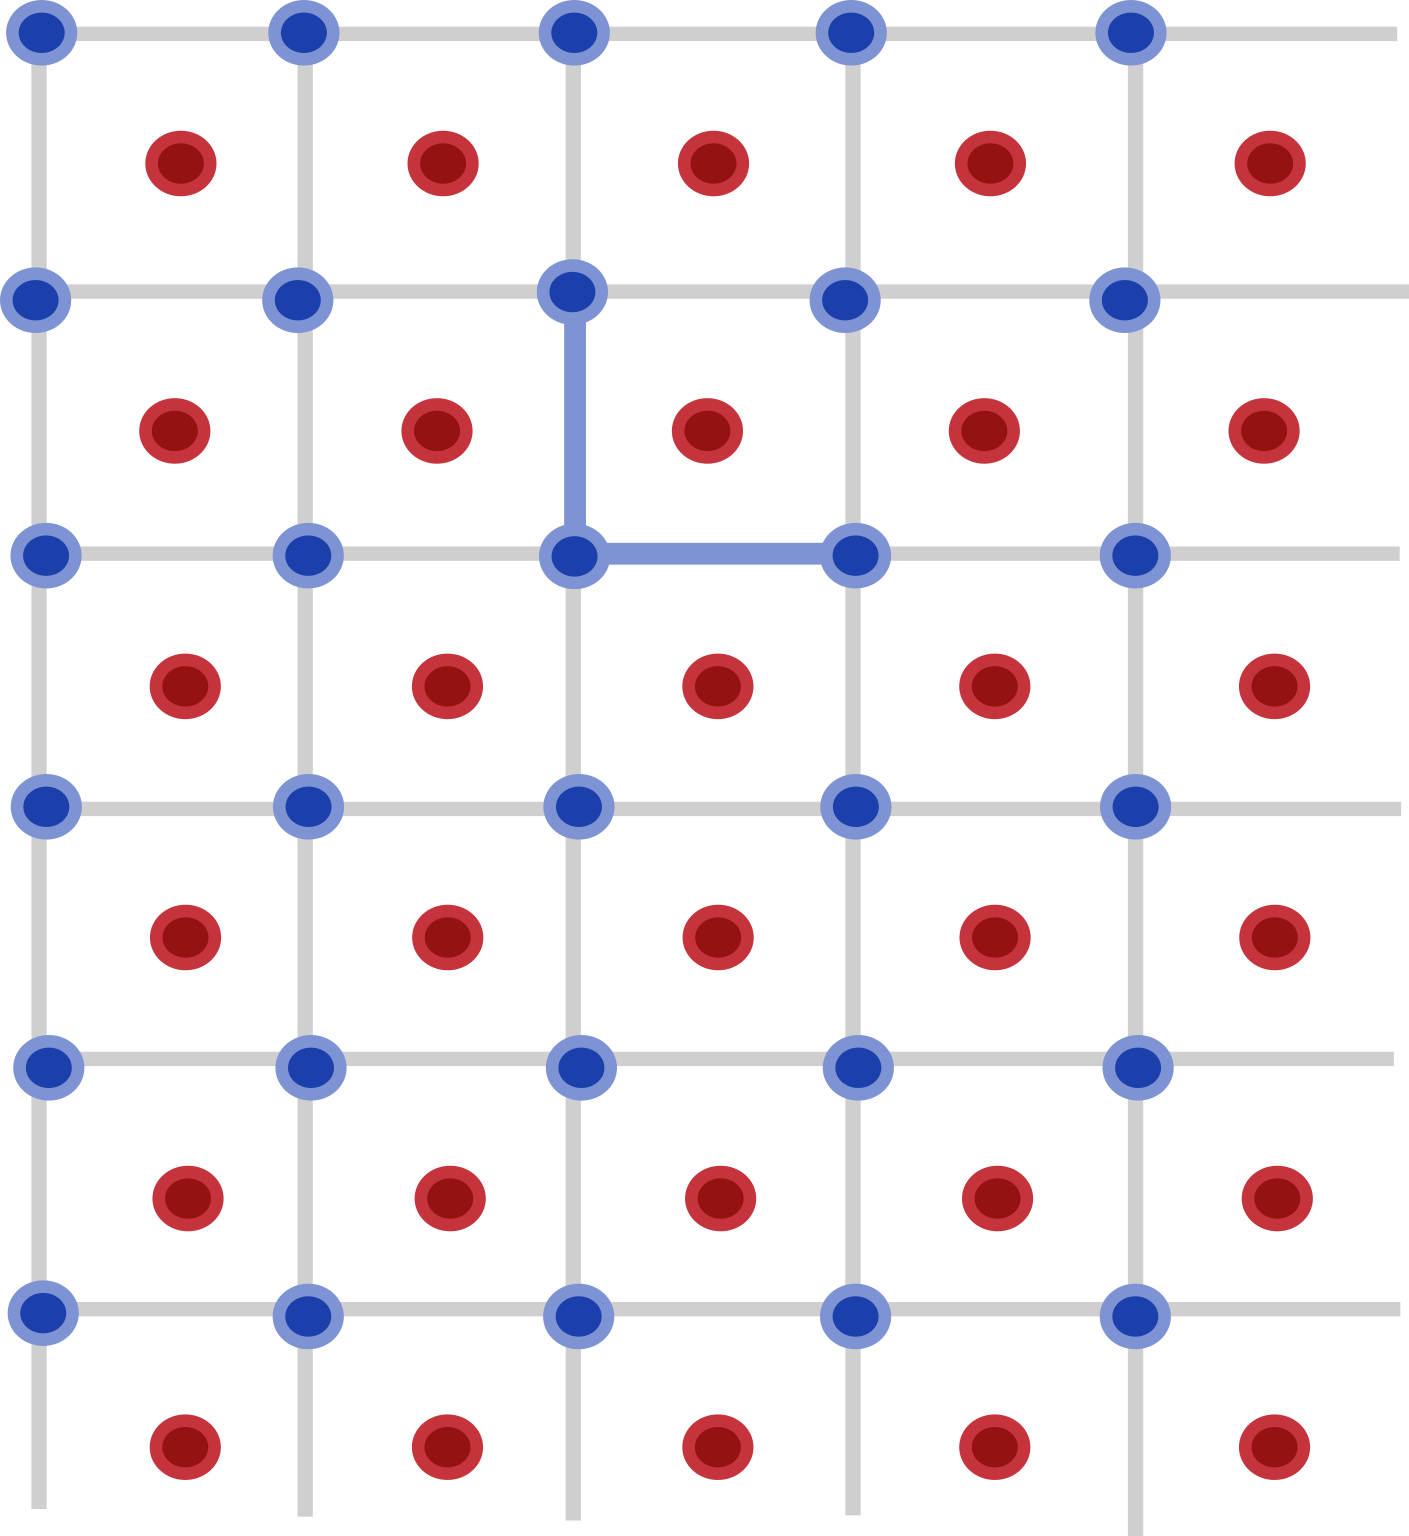
\includegraphics[width=0.35\textwidth]{fig/Toric_code_ex_8.png}
% 		\end{textblock*}
% 		\begin{textblock*}{8cm}(8cm,2cm)
% 			\textbf{Maximum likelihood/optimal decoding}\\
% 			$C_{s} \in \mathcal{G}_{n}$ compatible with $s$\\
% 			$[C_{s}]=SC_{s}$ \\
% 			$s \mapsto C_{s}L_{\delta(s)}$ with \\
% 			$\delta(s) = \arg\max_{l\in L}P([C_{s}L_{l}])$\\
% 			$\phantom{\delta(s)} \overset{\text{\cite{dennis_topological_2002}}}{=} \arg\max_{l\in L}Z^{T_{\text{Nishimori}}}(C_{s}L_{l})$
% 		\end{textblock*}
% 	}
% 	\only<9-9>{
% 		\begin{textblock*}{16cm}(2cm,1.7cm)
% 			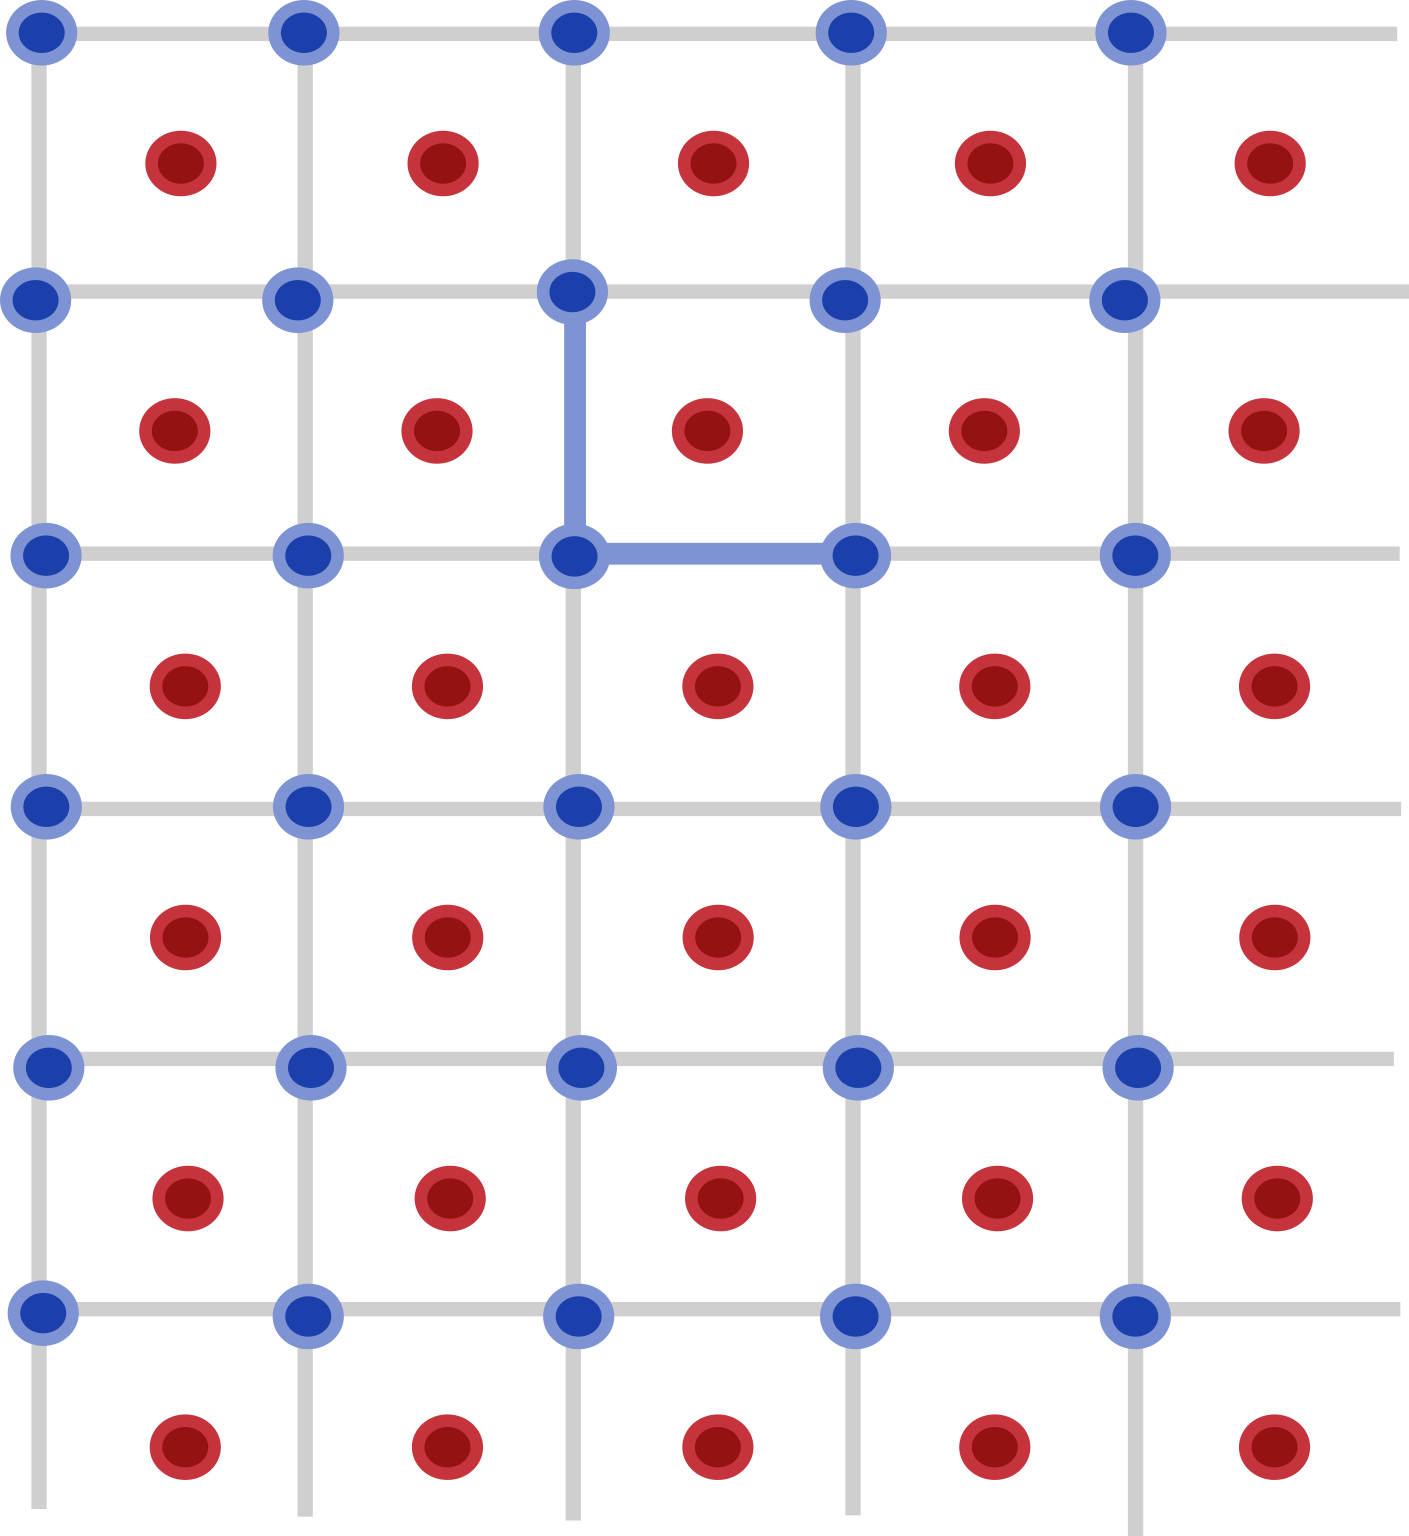
\includegraphics[width=0.35\textwidth]{fig/Toric_code_ex_8.png}
% 		\end{textblock*}
% 		\begin{textblock*}{8cm}(8cm,2cm)
% 			\textbf{Max Z decoding at temperature T}\\
% 			$C_{s} \in \mathcal{G}_{n}$ compatible with $s$\\
% 			$[C_{s}]=SC_{s}$ \\
% 			$s \mapsto C^{\star}_{s}(T)\equiv C_{s}L_{\delta(s)}$ with \\
% 			$\delta(s) = \arg\max_{l\in L}Z^{T}(C_{s}L_{l})$\\
% 			\vspace{0.8cm}
% 			\textbf{Probabilistic Z decoding at temperature T}:\\
% 			$\overline{\delta(s)}$ with $P(\overline{\delta(s)} = l\in L)=\frac{Z^{T}(C_{s}L_{l})}{\sum_{l\in L}Z^{T}(C_{s}L_{l})}$
% 		\end{textblock*}
% 	}
% 	\only<10-10>{
% 		\begin{textblock*}{16cm}(2cm,1.7cm)
% 			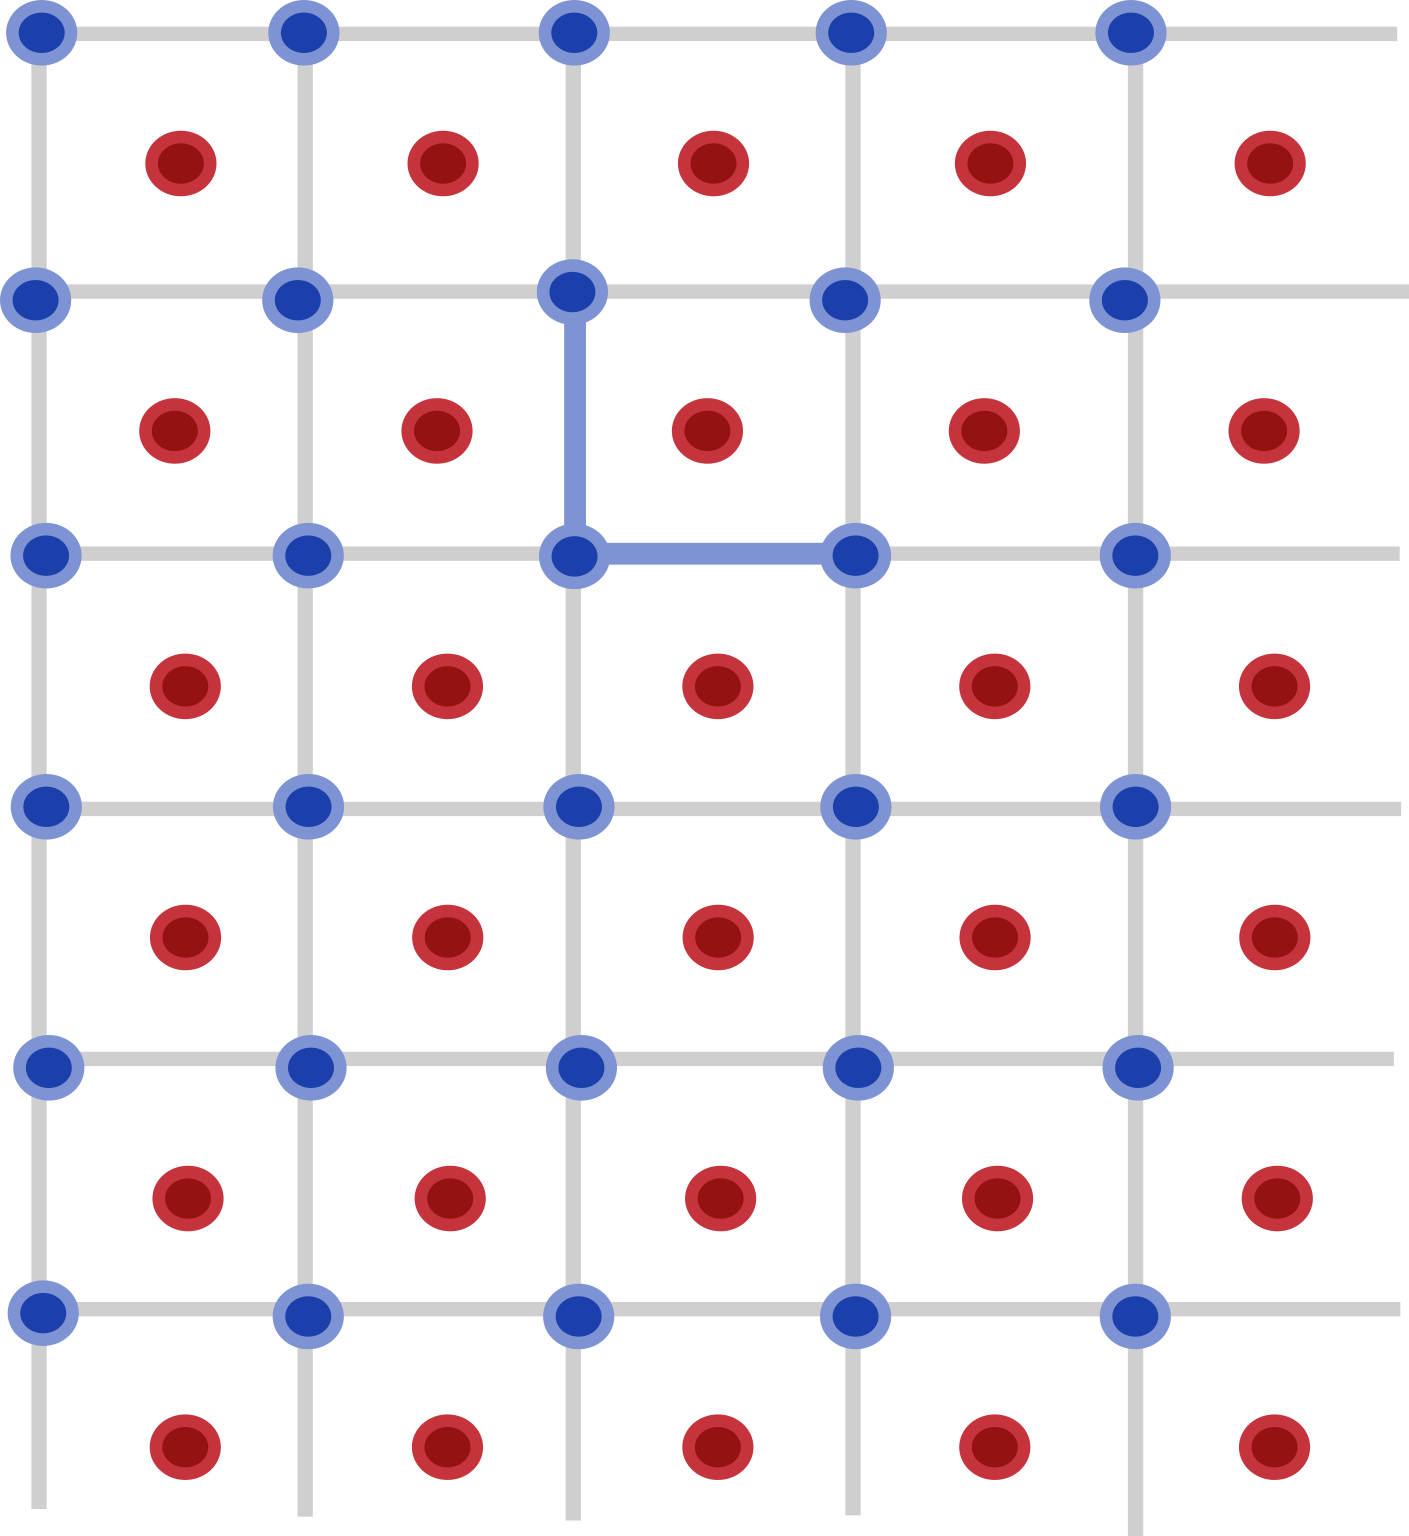
\includegraphics[width=0.35\textwidth]{fig/Toric_code_ex_8.png}
% 		\end{textblock*}
% 		\begin{textblock*}{8cm}(8cm,2cm)
% 			\textbf{Max Z decoding at temperature T}\\
% 			$C_{s} \in \mathcal{G}_{n}$ compatible with $s$\\
% 			$[C_{s}]=SC_{s}$ \\
% 			$s \mapsto C^{\star}_{s}(T)\equiv C_{s}L_{\delta(s)}$ with \\
% 			$\delta(s) = \arg\max_{l\in L}Z^{T}(C_{s}L_{l})$\\
% 			\vspace{0.8cm}
% 			\textbf{Probabilistic Z decoding at temperature T}:\\
% 			$\overline{\delta(s)}$ with $P(\overline{\delta(s)} = l\in L)=\frac{Z^{T}(C_{s}L_{l})}{\sum_{l\in L}Z^{T}(C_{s}L_{l})}$\\
% 			\vspace{0.8cm}
% 			Estimation of Z by REWL and FKT algorithm
% 		\end{textblock*}
% 	}
% 	% \only<6-6>{
% 	% \begin{textblock*}{16cm}(4cm,1.7cm)
% 	% 	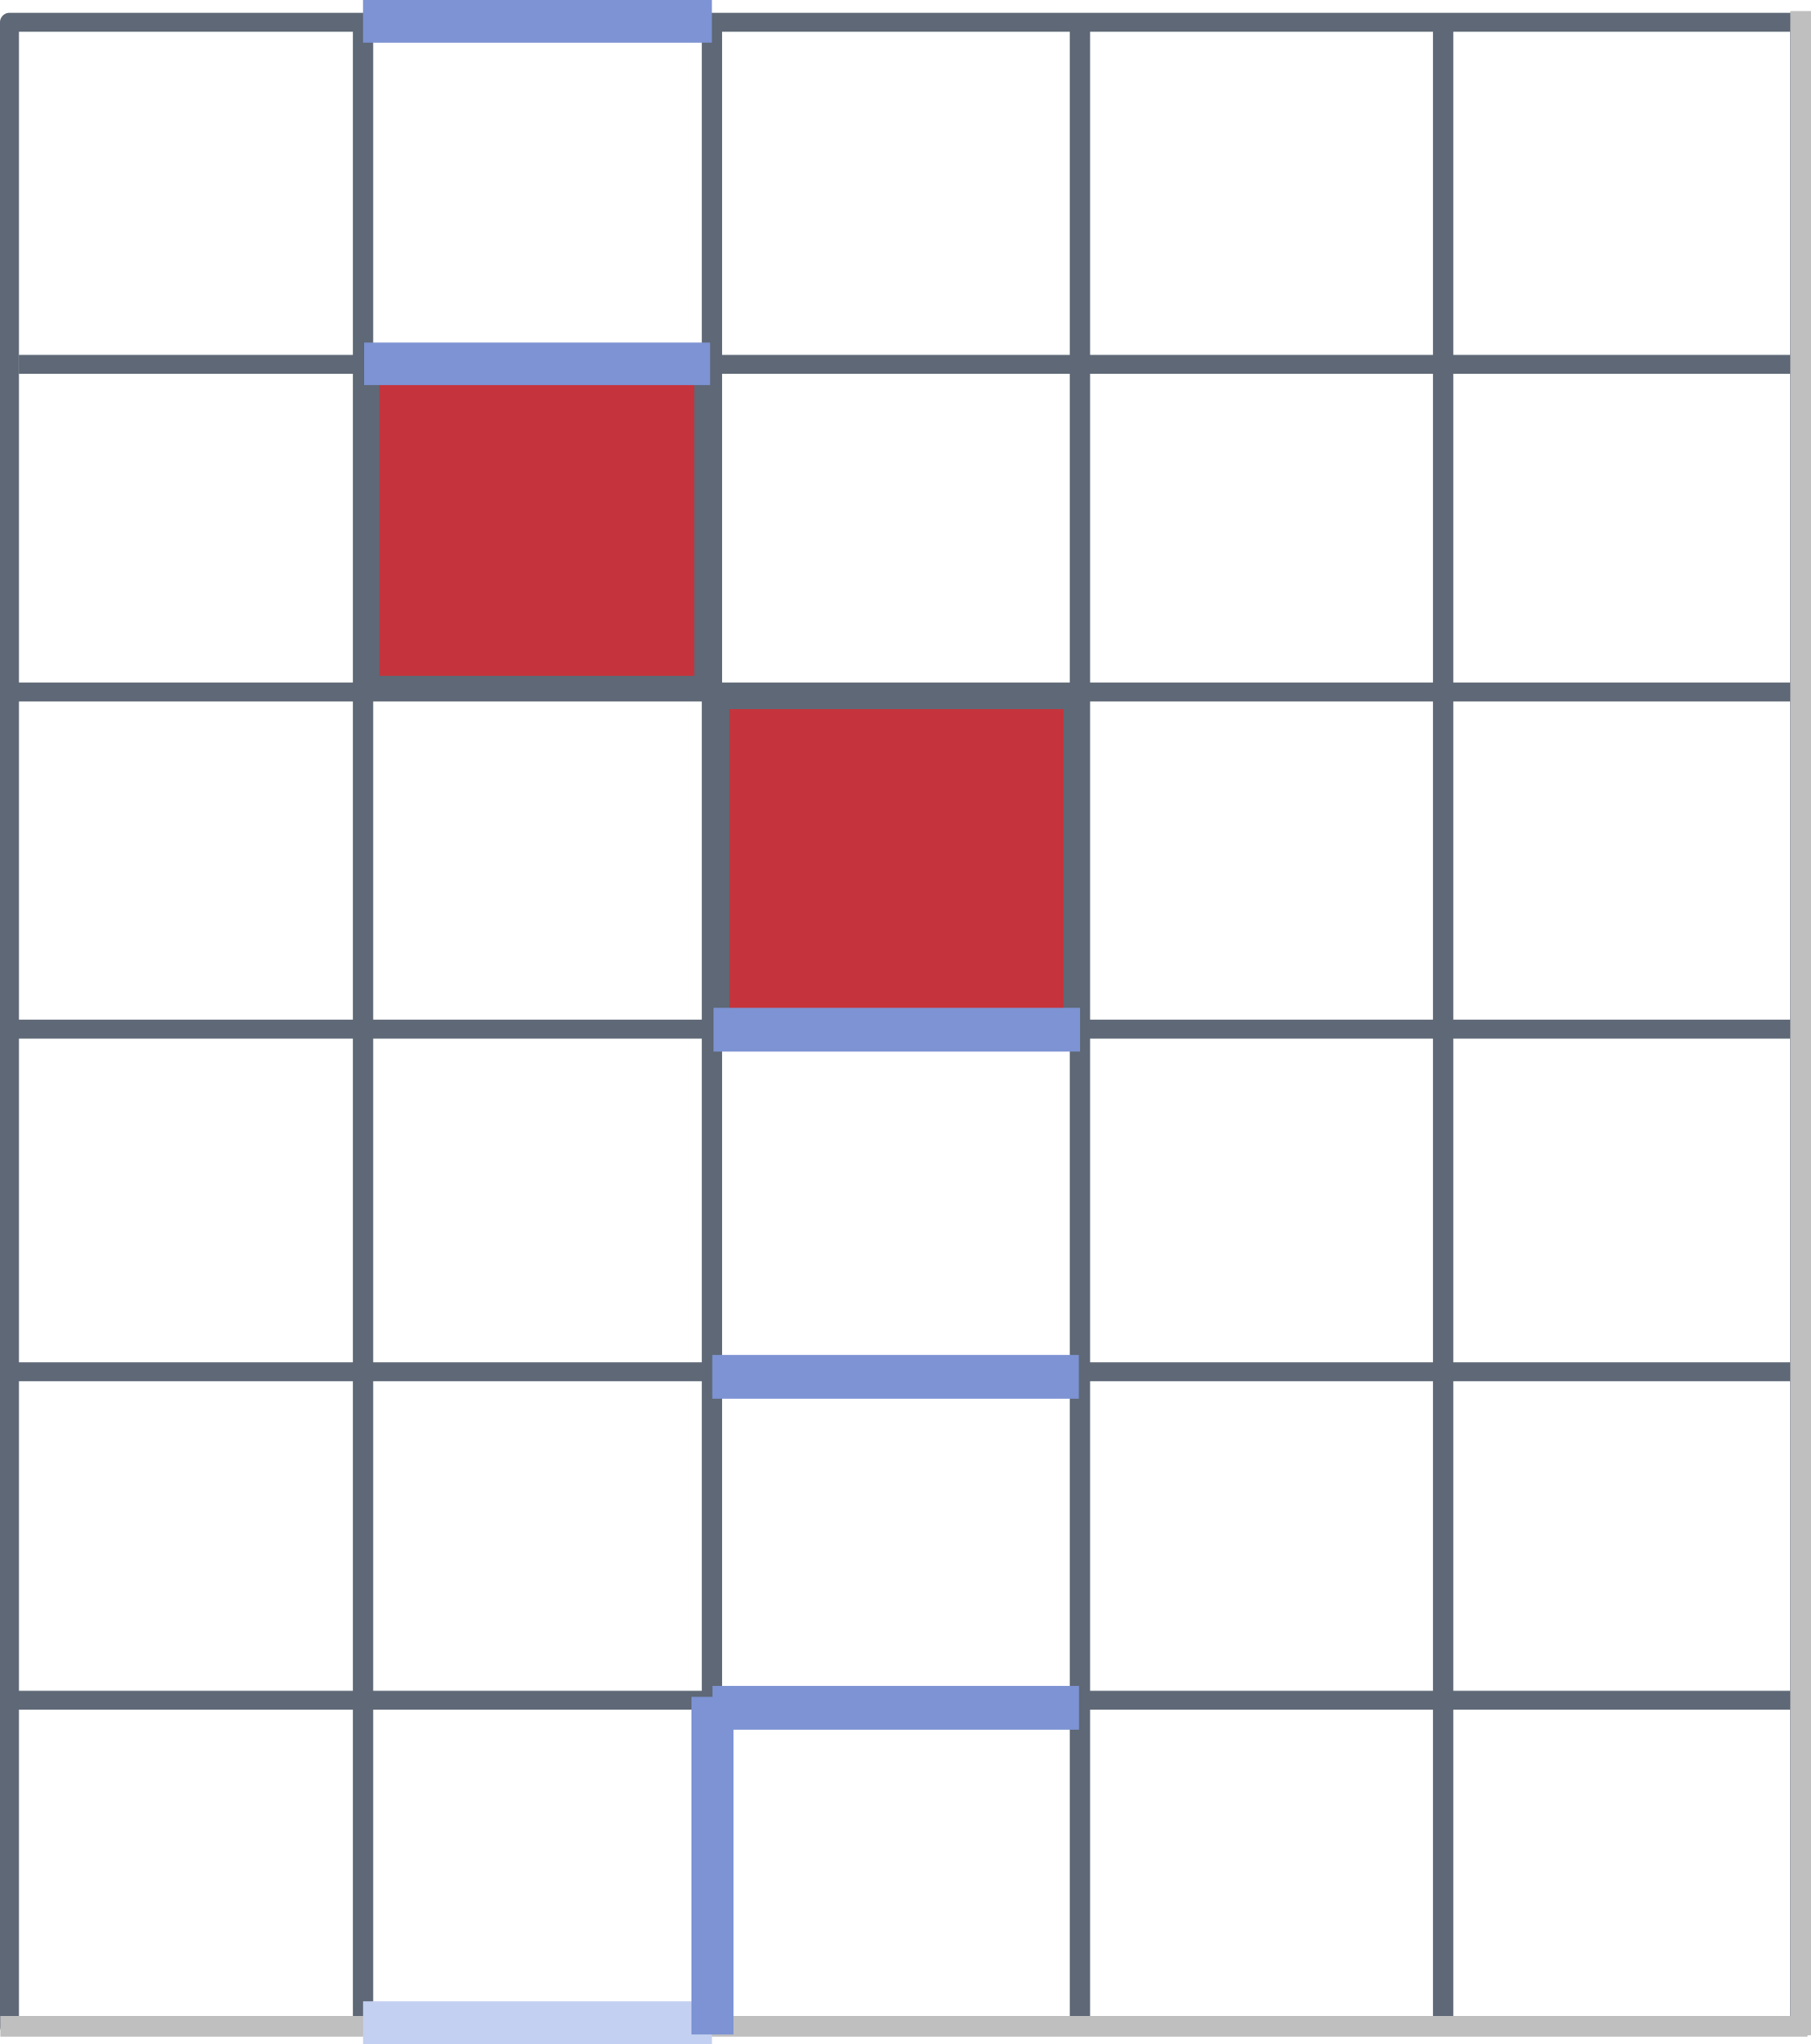
\includegraphics[width=0.35\textwidth]{fig/Toric_code_ex_4.png}
% 	% \end{textblock*}
% 	% }
% 	% \only<7-7>{
% 	% \begin{textblock*}{16cm}(4cm,1.7cm)
% 	% 	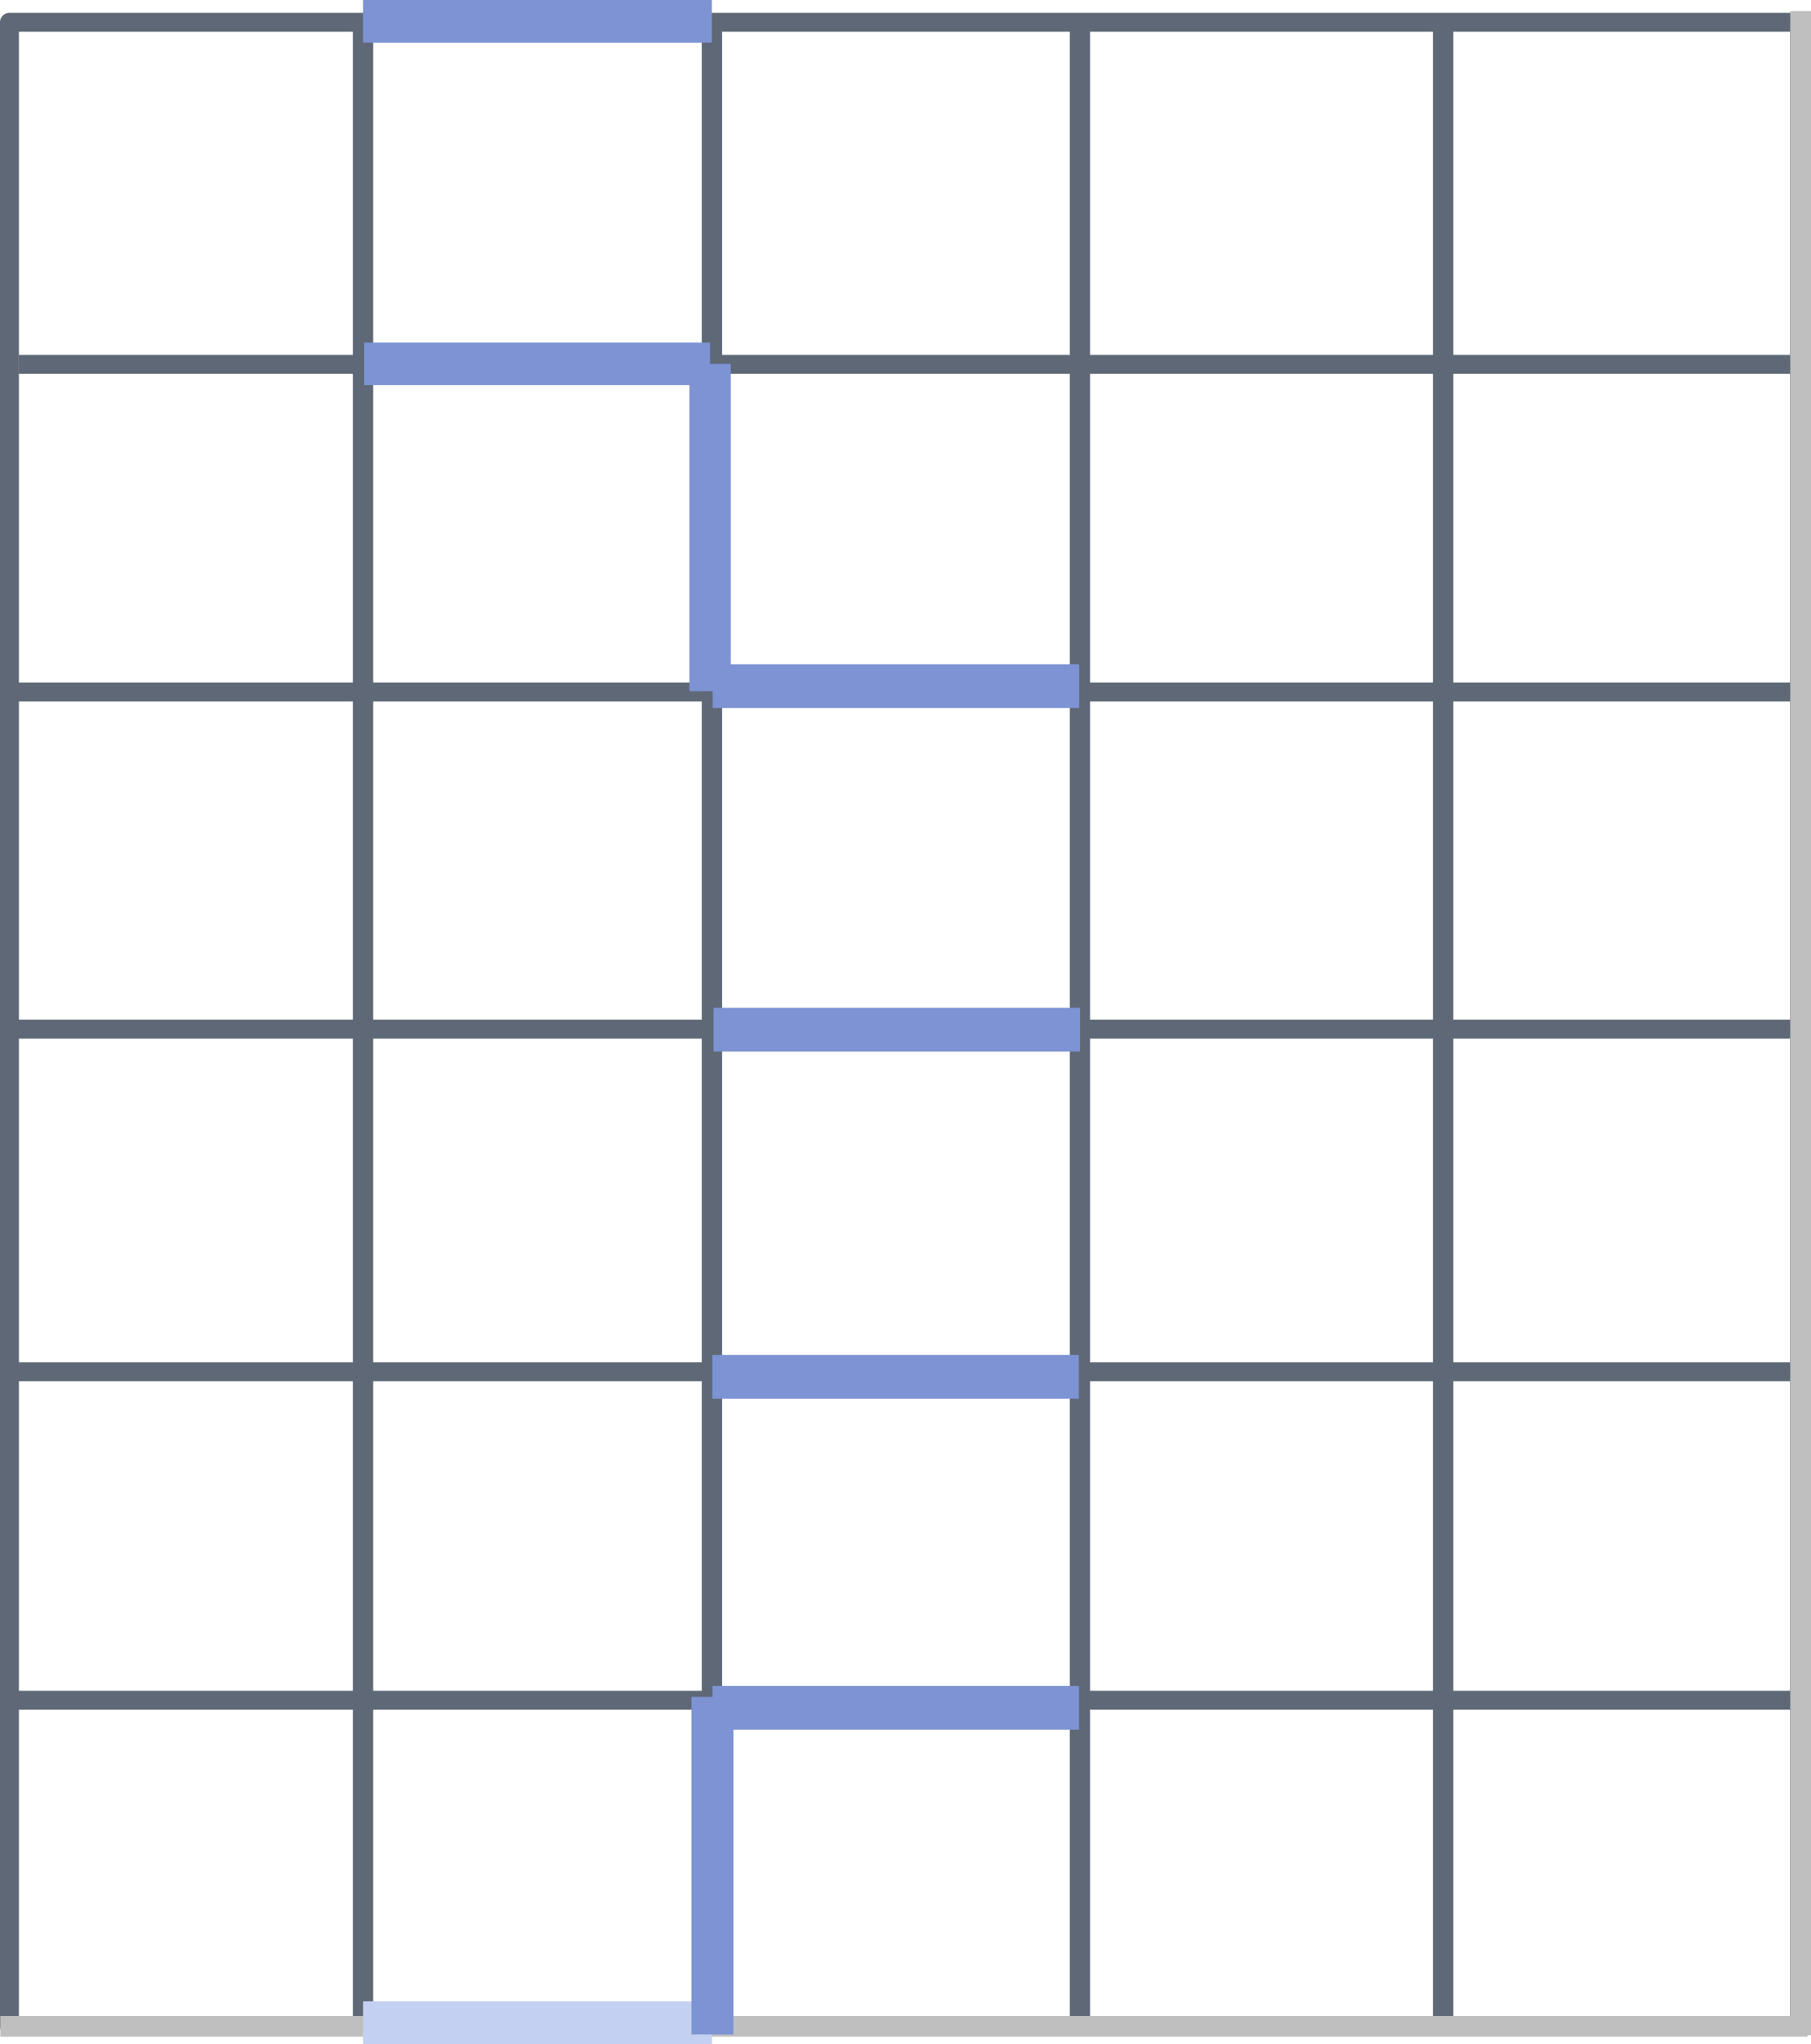
\includegraphics[width=0.35\textwidth]{fig/Toric_code_ex_5.png}
% 	% \end{textblock*}
% 	% }
% \end{frame}

% \begin{frame}{Definitions}
% 	\begin{minipage}{0.48\textwidth}
% 		\small
% 		\textbf{Z decoding at T}
% 		\begin{align*}
% 			&P_{\text{success}}=\sum_{s}P(s)P_{\text{success}}(s)\\
% 			&P_{\text{success}}(s)=P(C^{\star}_{s}(T))=\frac{Z^{T_{\text{Nishimori}}}(C^{\star}_{s})}{\sum_{l\in L}Z^{T_{\text{Nishimori}}}(C^{\star}_{s}L_{l})}\\
% 			&\Rightarrow P_{\text{success}}=\langle\frac{Z^{T_{\text{Nishimori}}}(C^{\star}_{s})}{\sum_{l\in L}Z^{T_{\text{Nishimori}}}(C^{\star}_{s}L_{l})}\rangle_{s}
% 		\end{align*}
% 		with $[C^{\star}_{s}(T)]: Z^{T}(C^{\star}_{s})\geq Z^{T}(C_{s})$
%     \end{minipage}
% \end{frame}

% \begin{frame}{Intermezzo - Groundwork for Results}
% 	\begin{minipage}{0.48\textwidth}
% 		\small
% 		\textbf{Max Z decoding at T}
% 		\begin{align*}
% 			&P_{\text{success}}=\langle\frac{Z^{T_{\text{Nishimori}}}(C^{\star}_{s})}{\sum_{l\in L}Z^{T_{\text{Nishimori}}}(C^{\star}_{s}L_{l})}\rangle_{s}
% 		\end{align*}
% 		with $[C^{\star}_{s}(T)]: Z^{T}(C^{\star}_{s})\geq Z^{T}(C_{s})$
%     \end{minipage}
%     \hfill
% 	\pause
%     \begin{minipage}{0.48\textwidth}
%         \small
% 		\textbf{Probabilistic Z decoding at T}
% 		\begin{align*}
% 			&P_{\text{success}}=\langle\frac{Z^{T}(C_{s}L_{\bar{l}})}{\sum_{l\in L}Z^{T}(C_{s}L_{l})}\rangle_{s}
% 		\end{align*}
% 		with $P(\bar{l}=l)=\frac{Z^{T}(C_{s}L_{l})}{\sum_{l\in L}Z^{T}(C_{s}L_{l})}$
%     \end{minipage}
% 	\pause
% 	\textcolor{red}{\textbf{Decoding probability}}
% 	\hspace{3cm}
% 	\textcolor{red}{\textbf{Order probability}}
% \end{frame}

\begin{frame}{Preliminary Results}
	\only<1-1>{
	\begin{textblock*}{14cm}(1.5cm,2cm)
		\raisebox{-0.7cm}{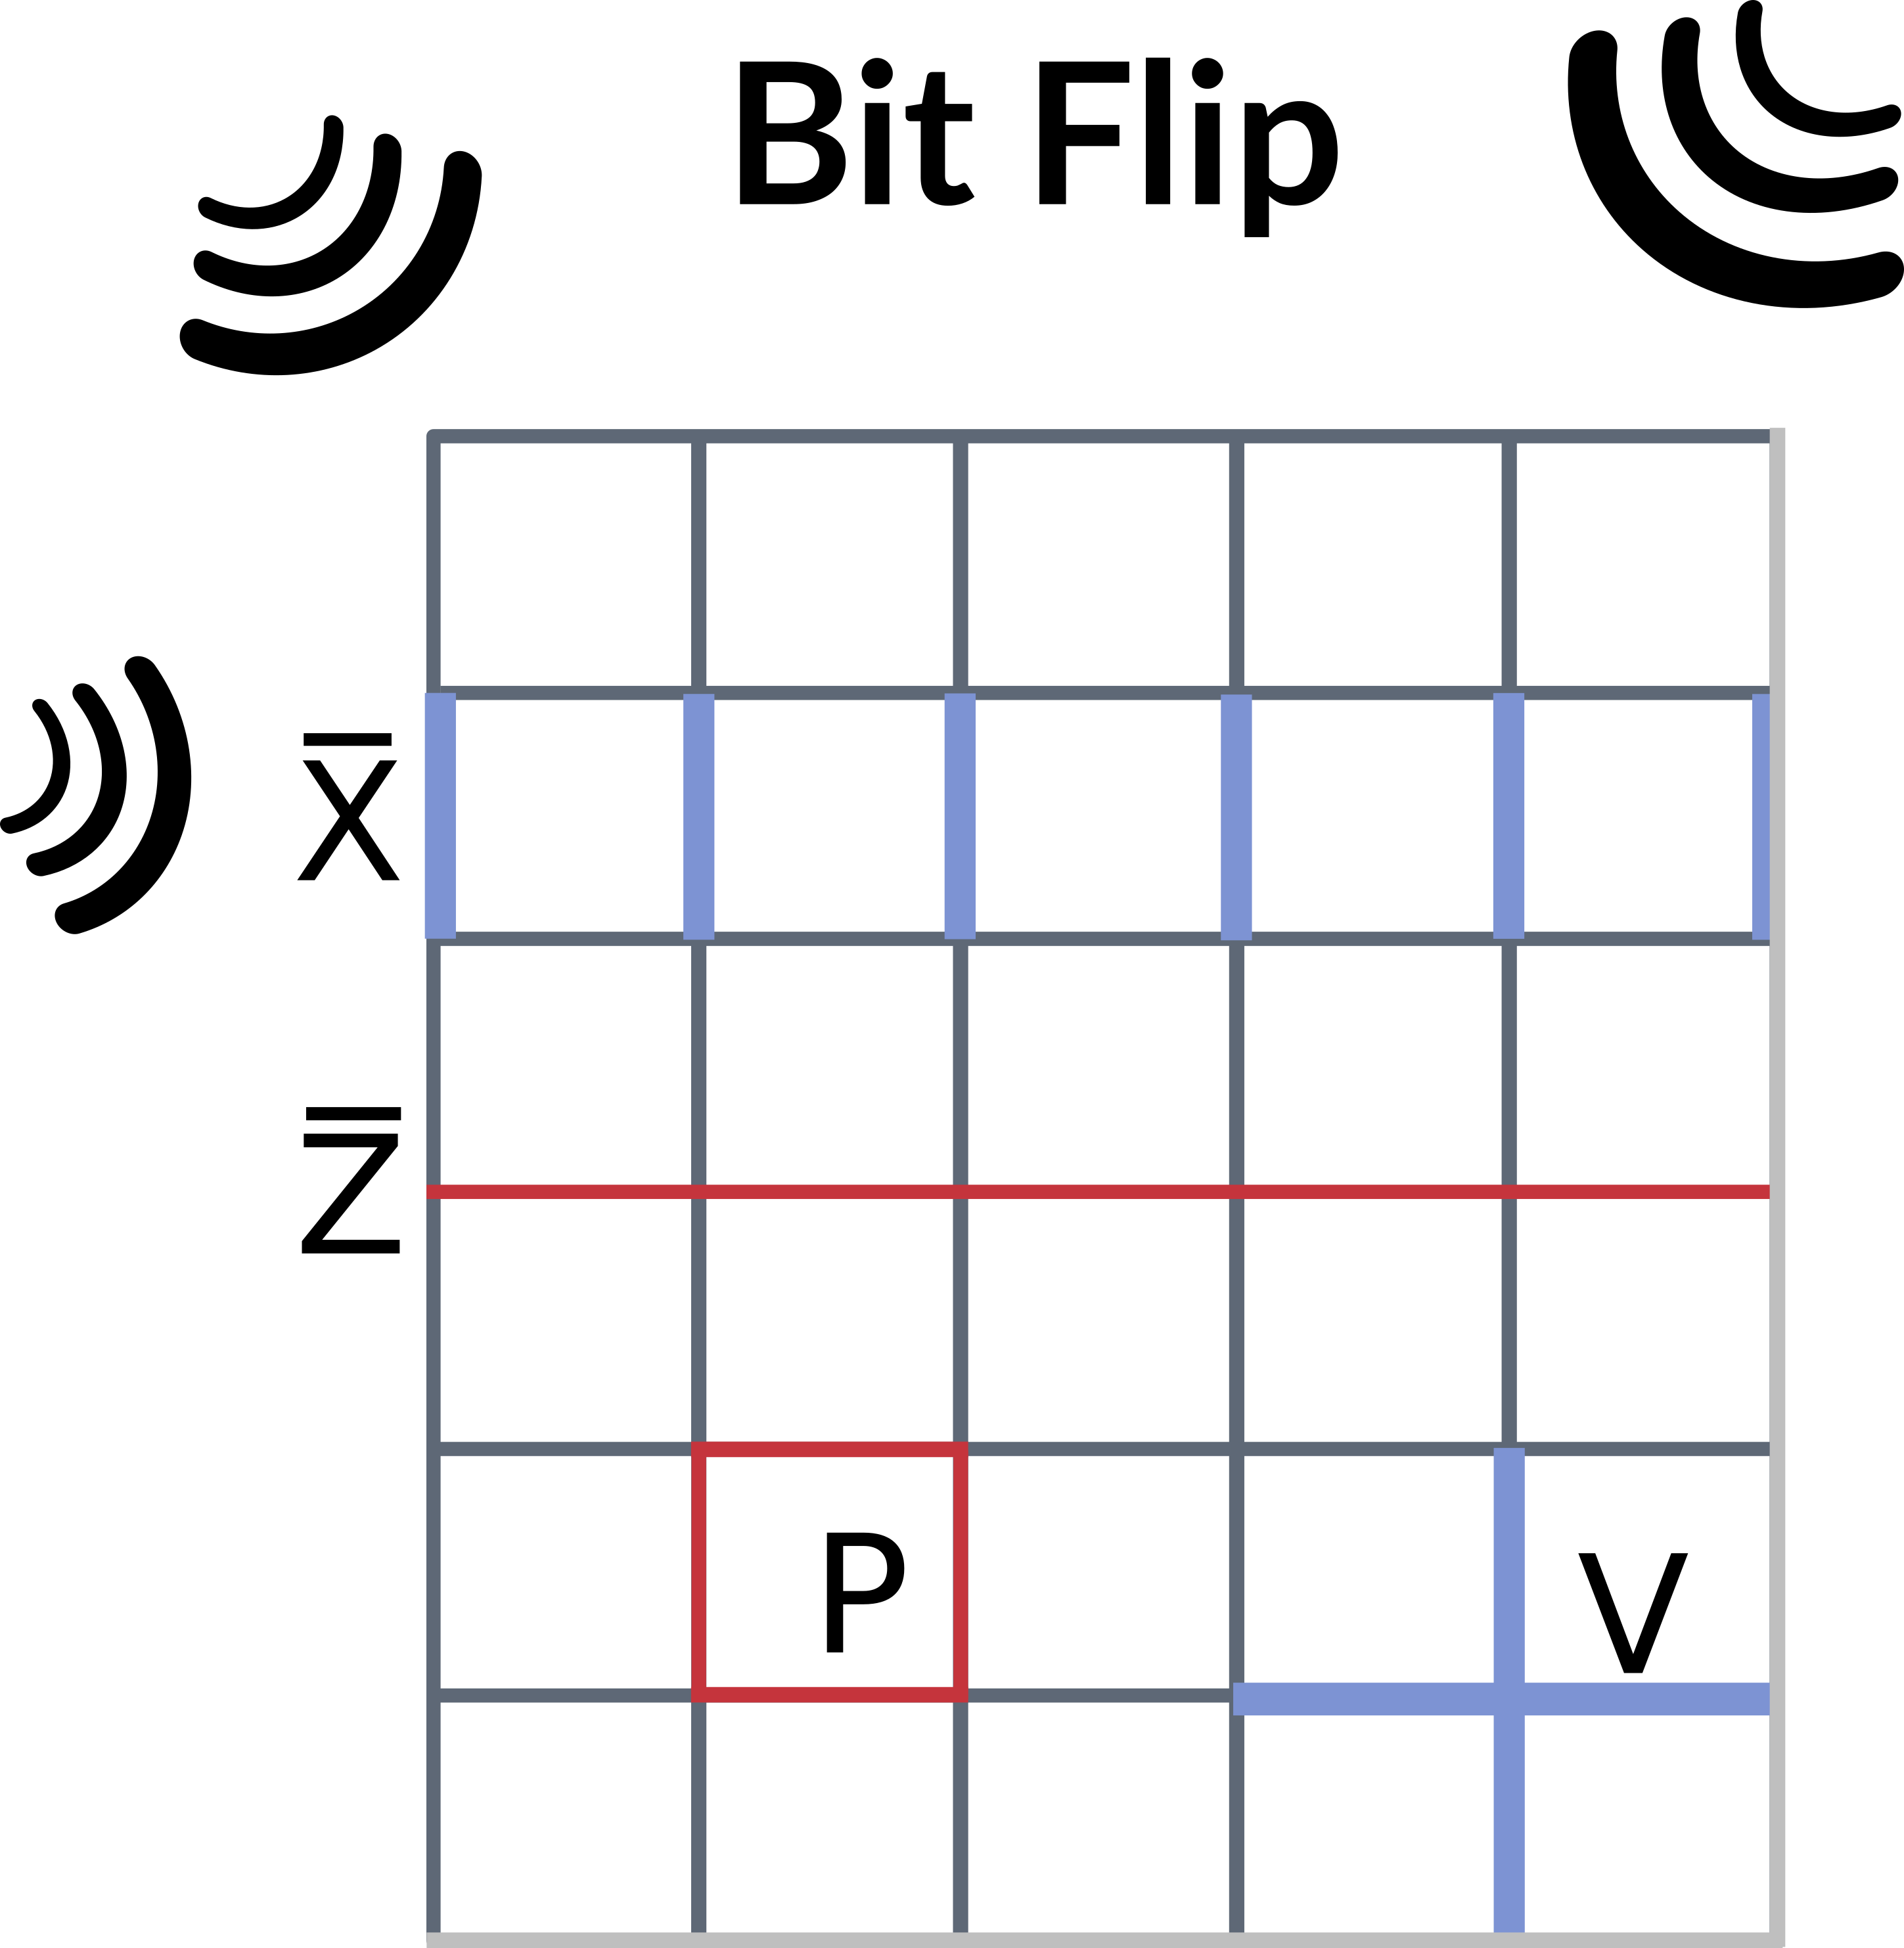
\includegraphics[width=0.15\textwidth]{fig/toric_code.png}}
		\begin{tikzpicture}[overlay]
			\draw[->, line width=0.8mm, black] (0.5, 0.1) -- (4,0.1);
			\draw[-, line width=0.8mm, black] (0.5, 0.3) -- (0.5,-0.1);
		\end{tikzpicture}
		\hspace{4.5cm}
		Error class probability estimates
	\end{textblock*}
	}
	\pause
	\only<2-2>{
		\hspace{2cm}
		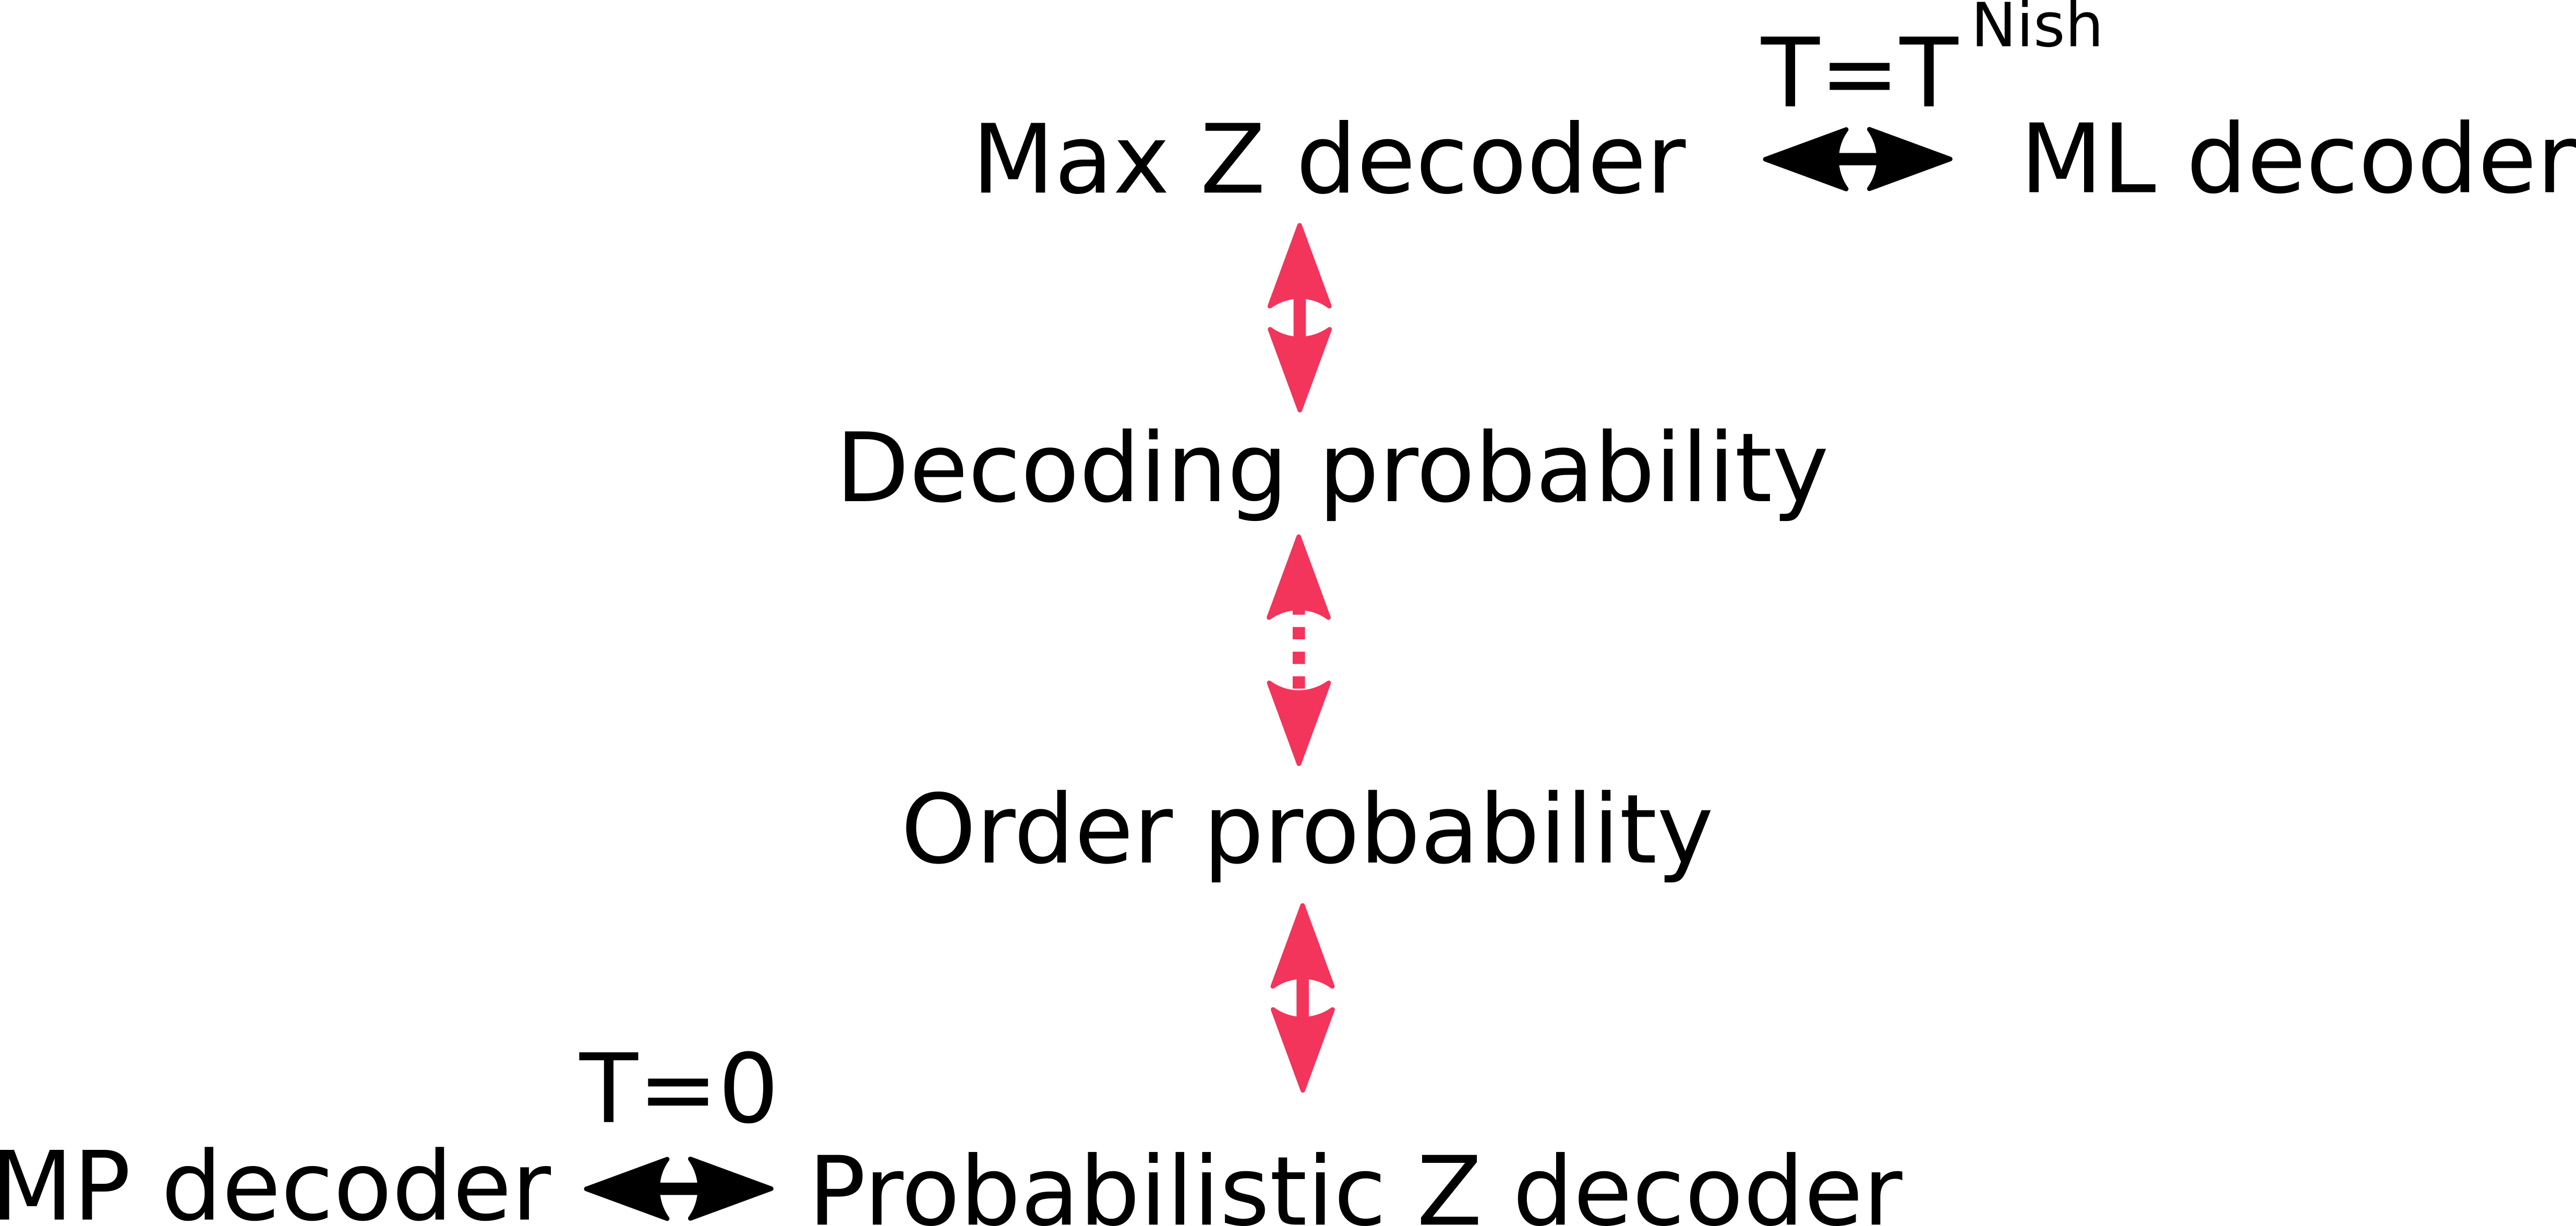
\includegraphics[width=0.7\textwidth]{fig/ML_MP.png}
	}
\end{frame}

\begin{frame}{Preliminary Results}
	\begin{figure}[h!]
		\centering
		\begin{minipage}{0.45\textwidth}
			\centering
			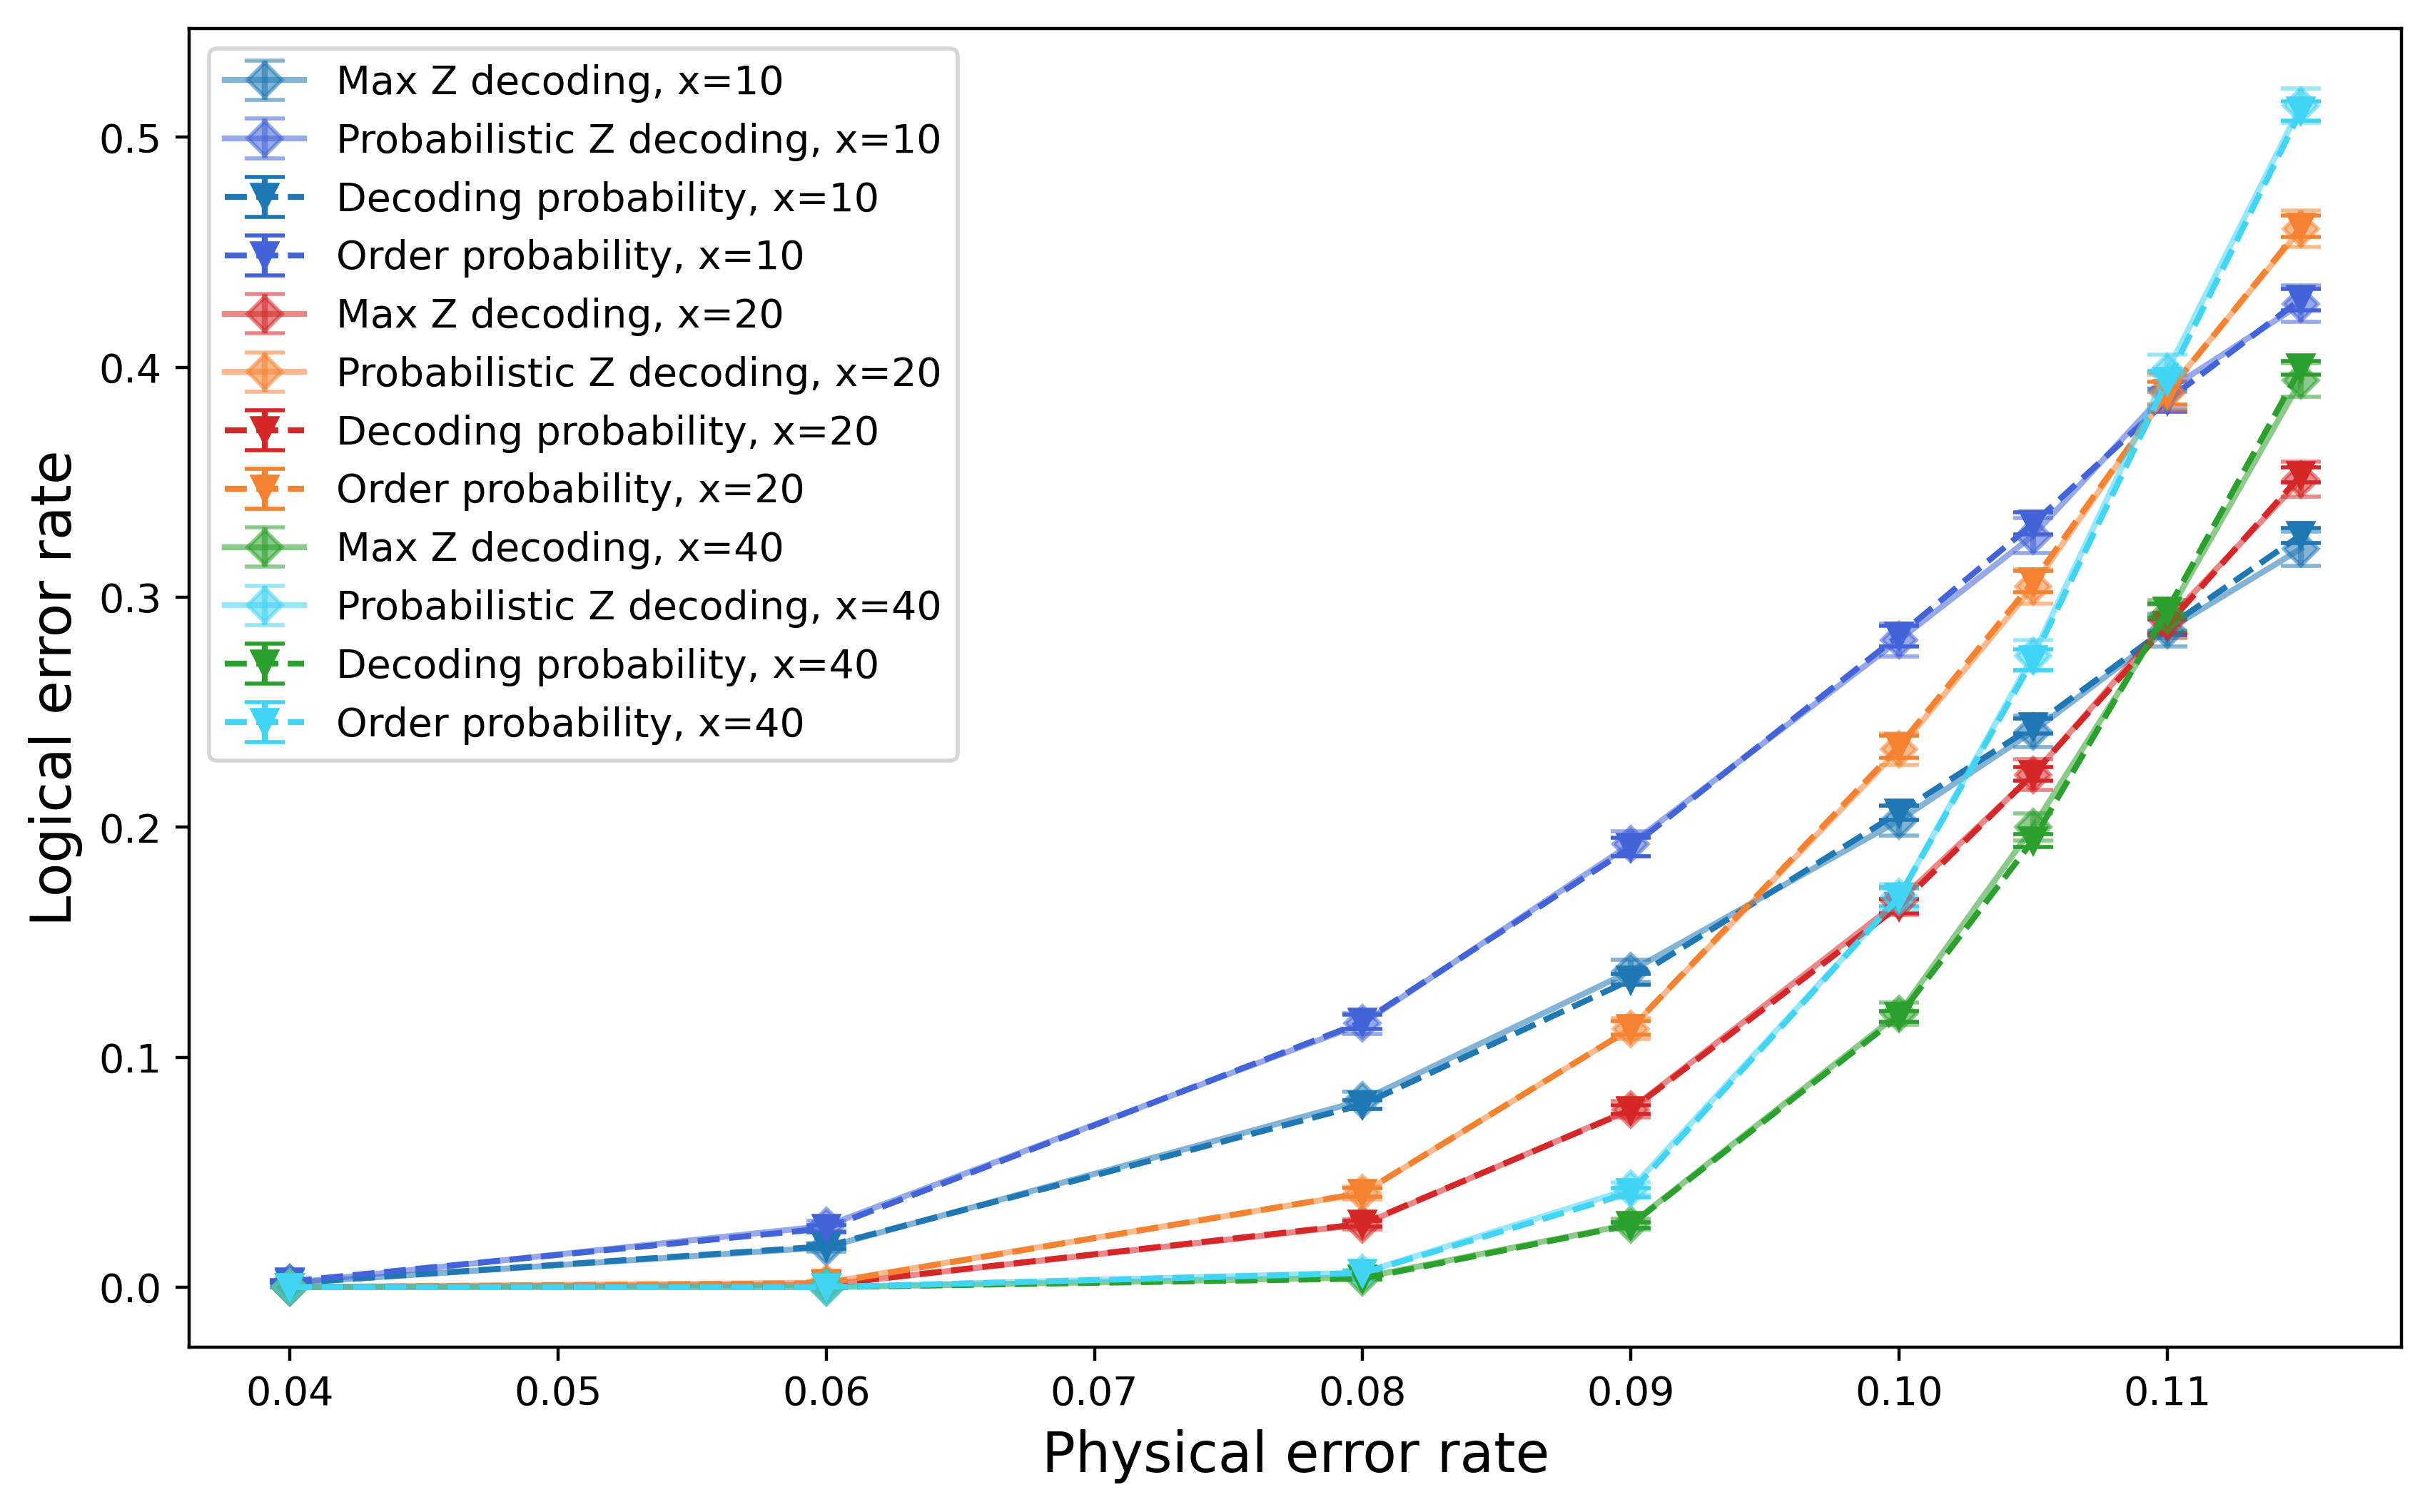
\includegraphics[width=\textwidth]{fig/MaxZ_ProbabilisticZ_OrderProb_DecodingProb_even_T1.png}
			\caption{Comparison efficient sampling methods to brute force decoding for even sizes at $T=T_{\text{Nish}}$}
		\end{minipage} \hfill
		\begin{minipage}{0.45\textwidth}
			\centering
			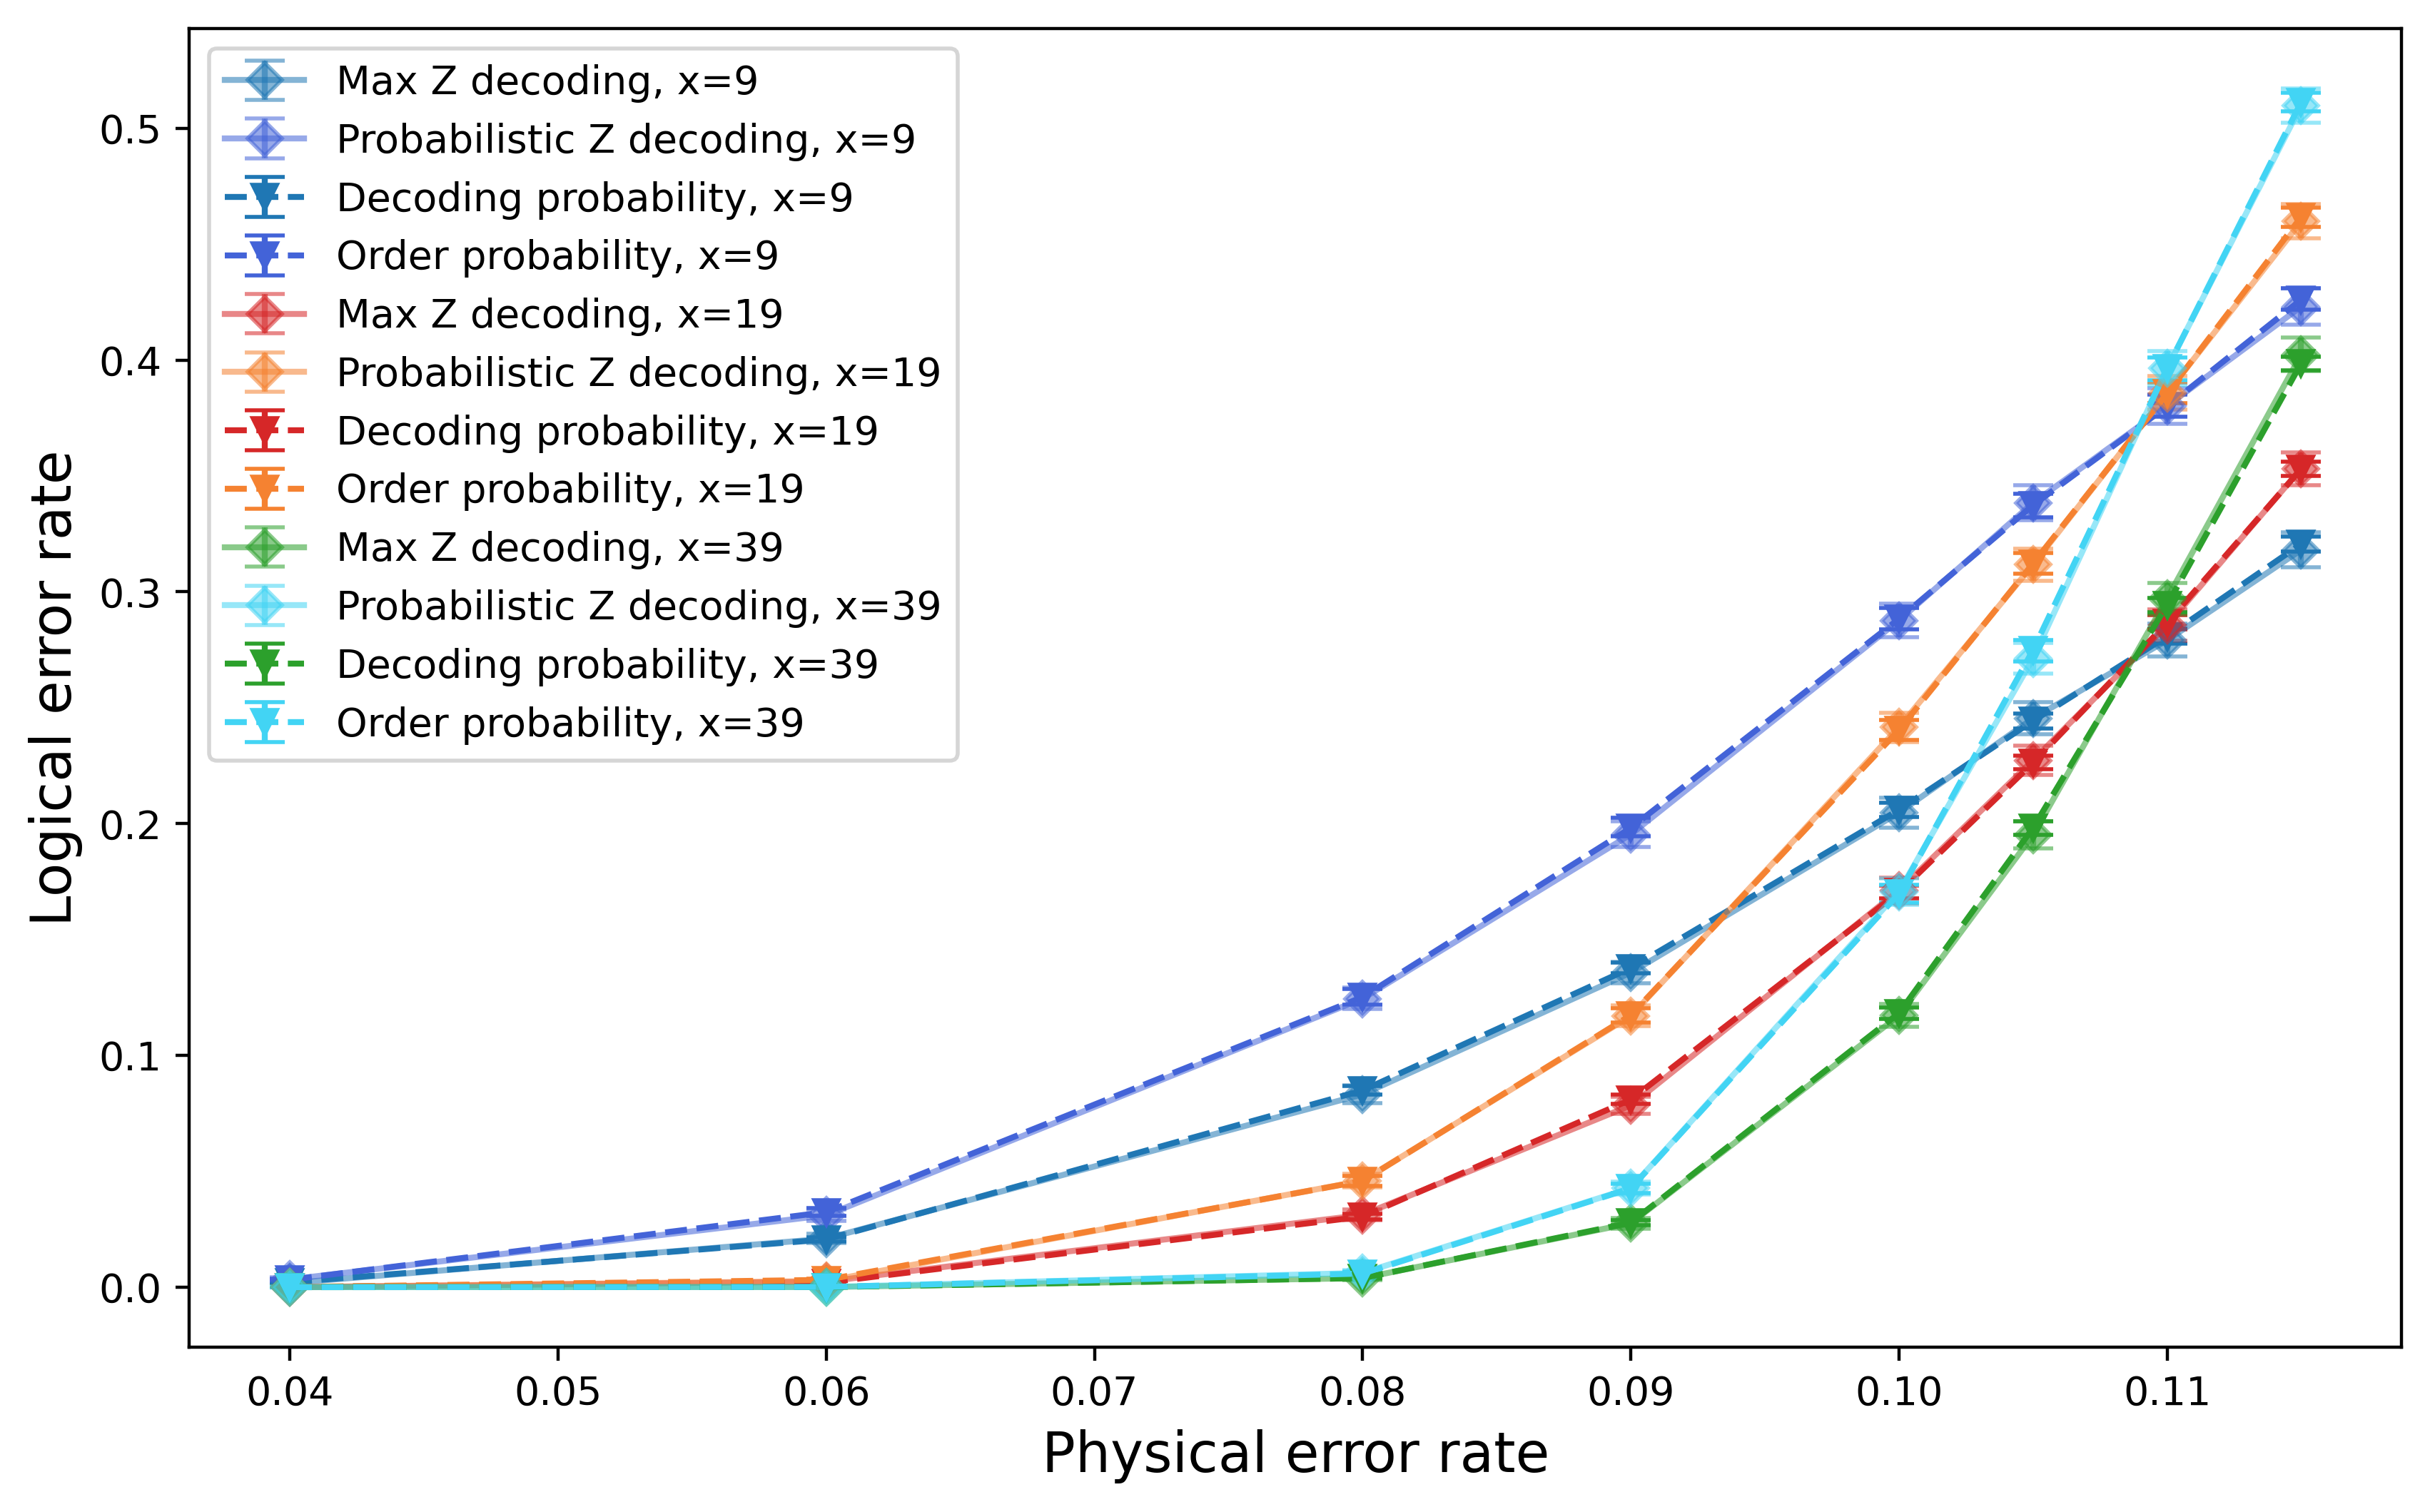
\includegraphics[width=\textwidth]{fig/MaxZ_ProbabilisticZ_OrderProb_DecodingProb_odd_T1.png}
			\caption{Comparison efficient sampling methods to brute force decoding for odd sizes at $T=T_{\text{Nish}}$}
		\end{minipage}
	\end{figure}
\end{frame}

\begin{frame}{Preliminary Results}
	\begin{figure}[h!]
		\centering
		\begin{minipage}{0.45\textwidth}
			\centering
			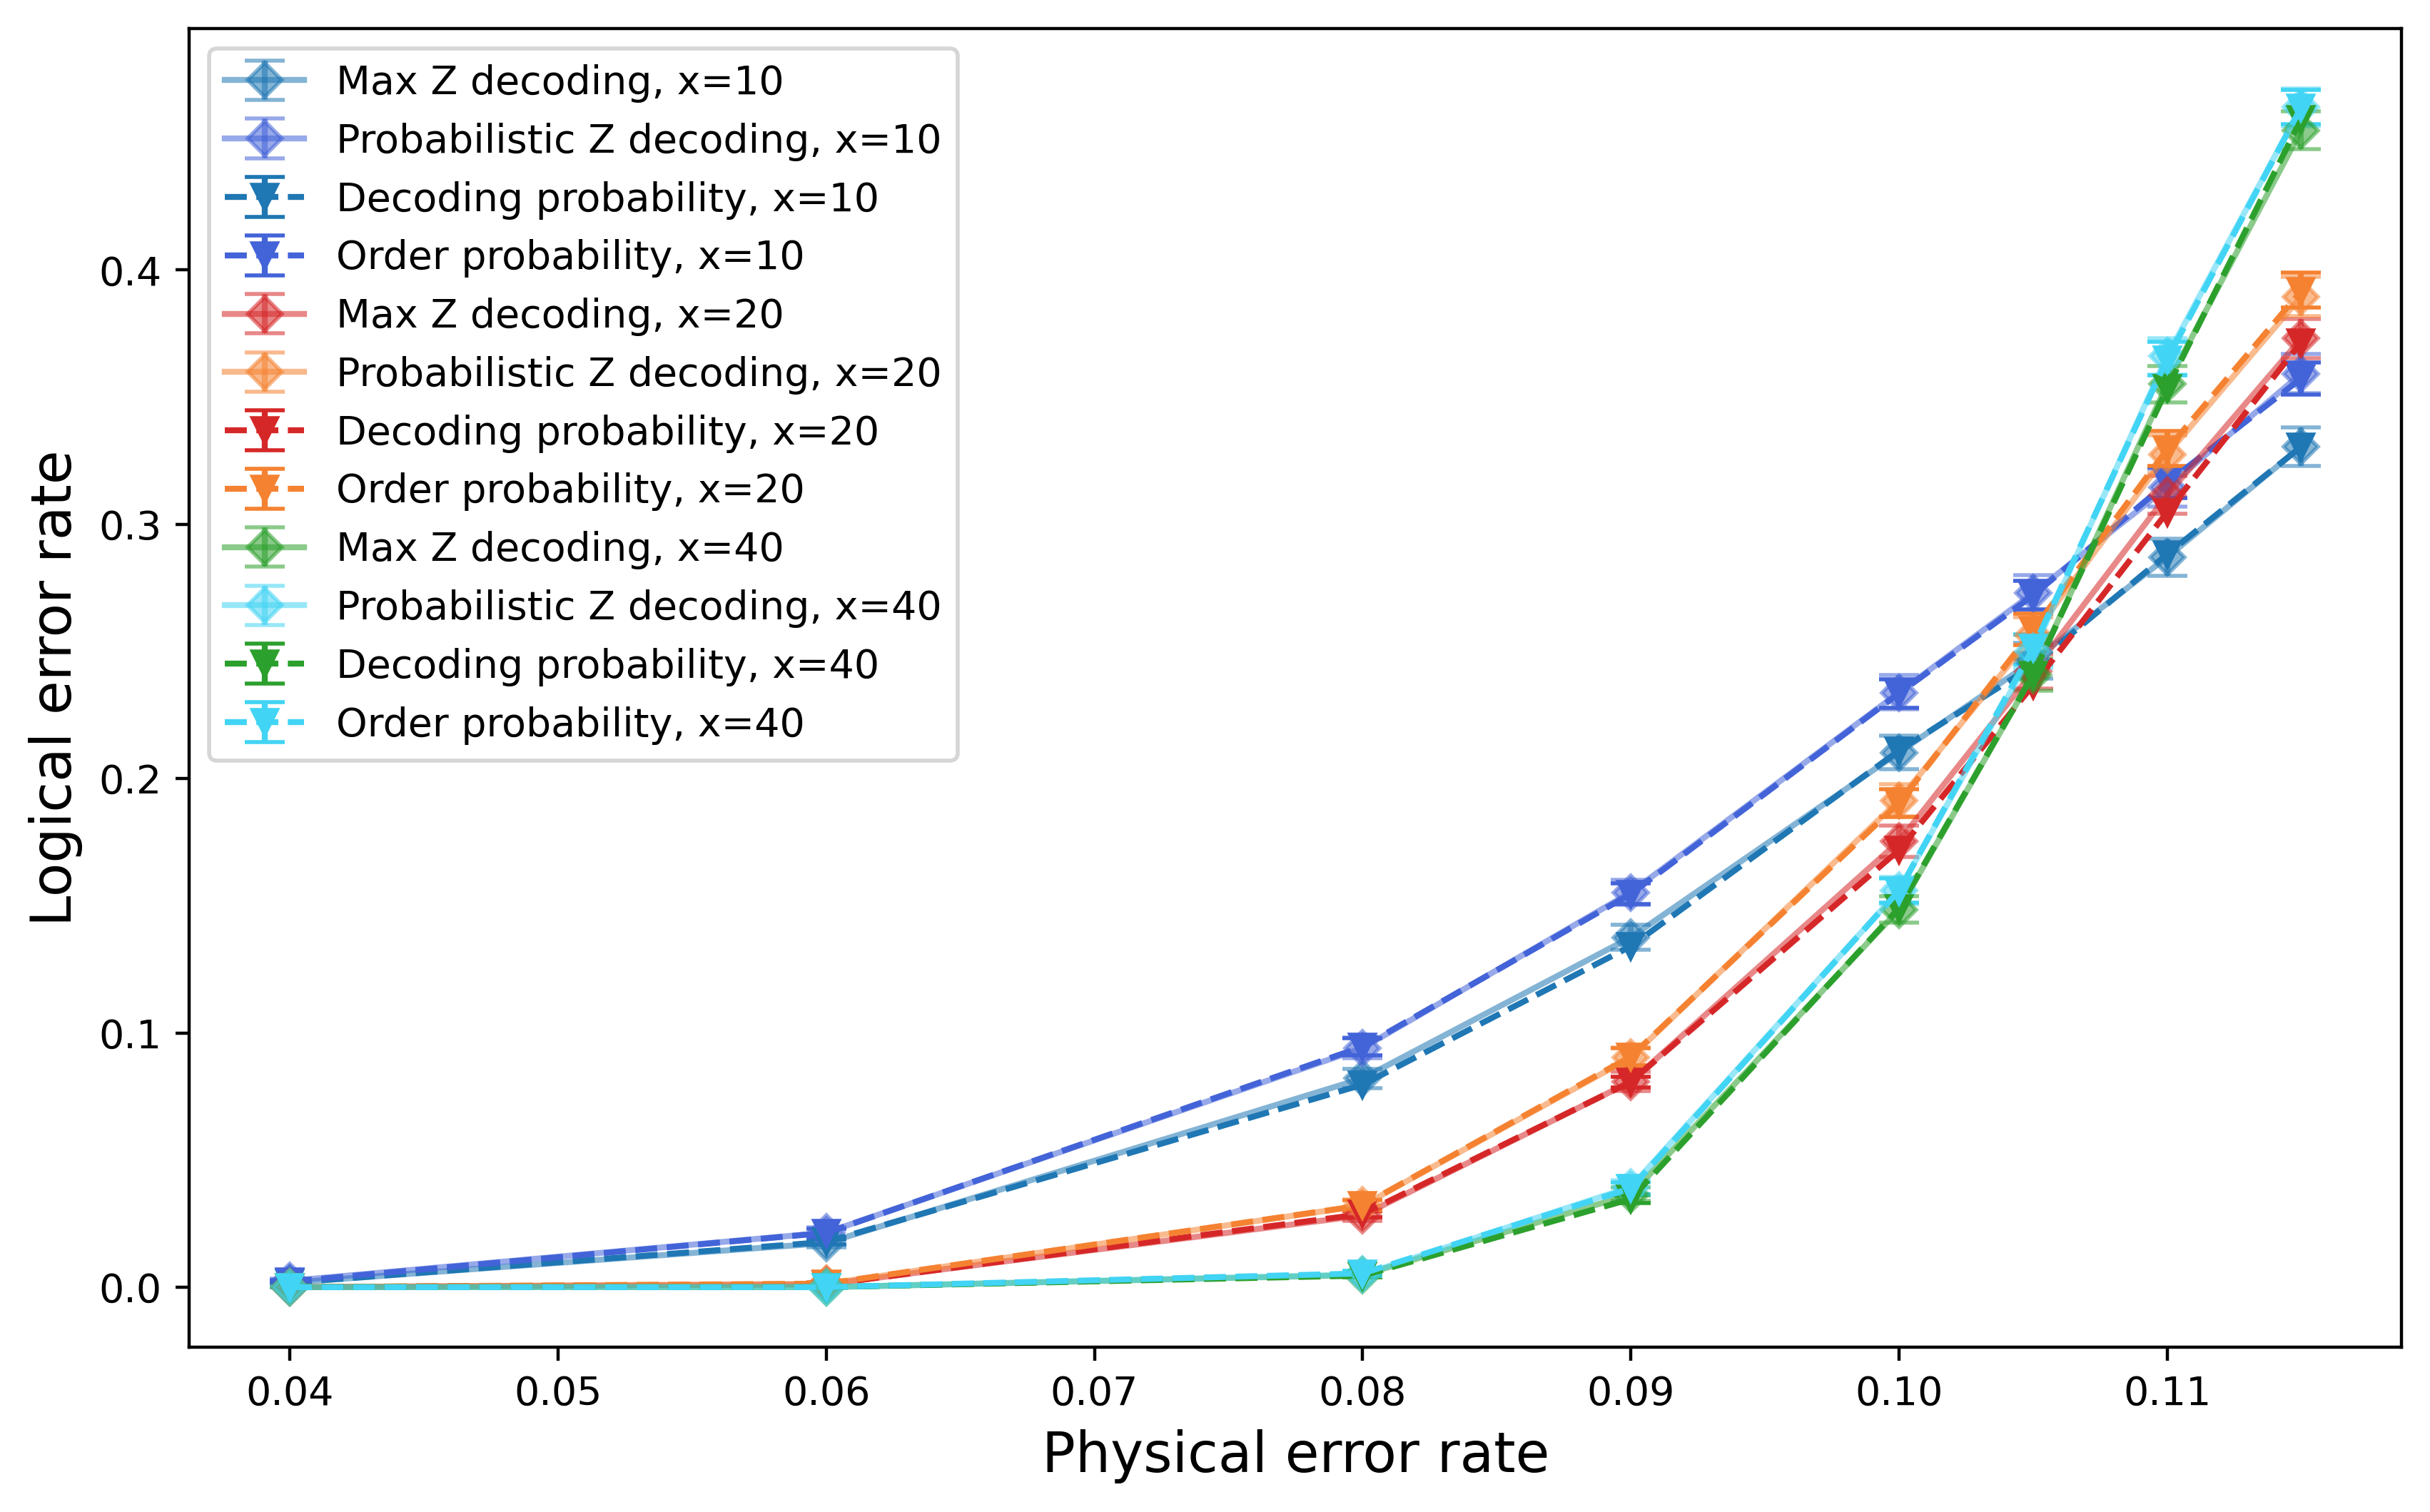
\includegraphics[width=\textwidth]{fig/MaxZ_ProbabilisticZ_OrderProb_DecodingProb_even_T01.png}
			\caption{Comparison efficient sampling methods to brute force decoding for even sizes at $T=0.1T_{\text{Nish}}$}
		\end{minipage} \hfill
		\begin{minipage}{0.45\textwidth}
			\centering
			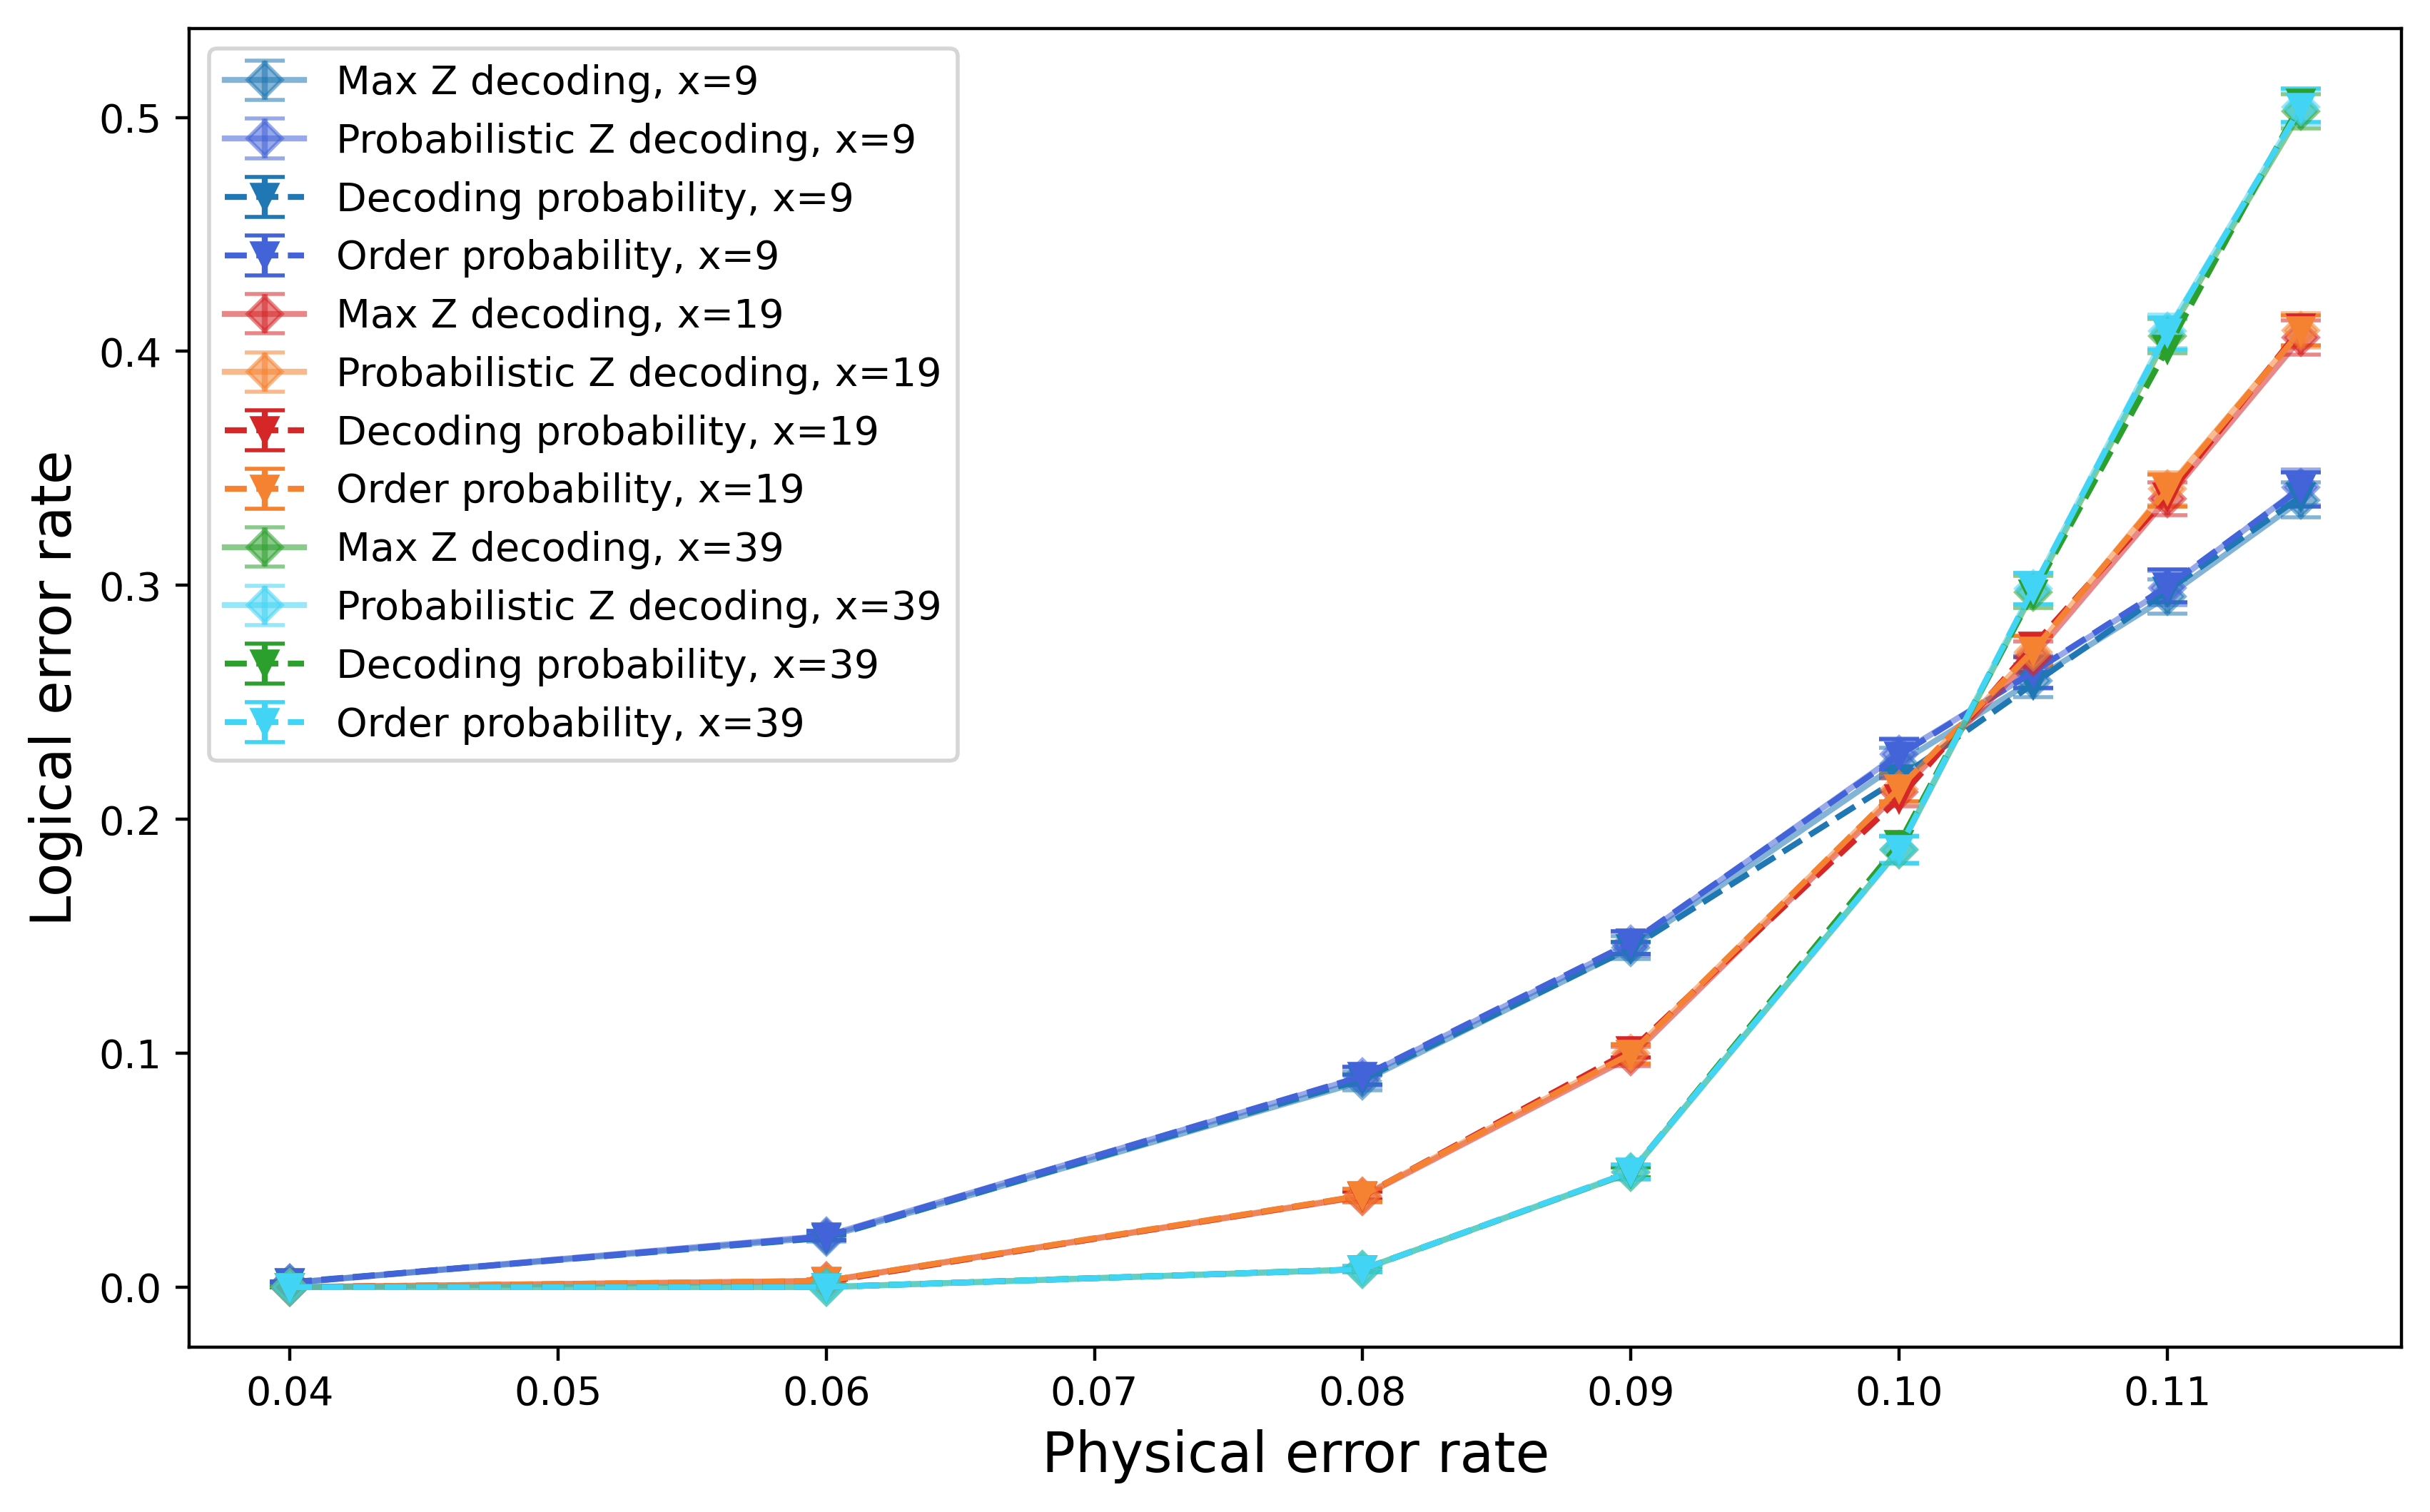
\includegraphics[width=\textwidth]{fig/MaxZ_ProbabilisticZ_OrderProb_DecodingProb_odd_T01.png}
			\caption{Comparison efficient sampling methods to brute force decoding for odd sizes at $T=0.1T_{\text{Nish}}$}
		\end{minipage}
	\end{figure}
\end{frame}

\begin{frame}{Preliminary Results}
	\begin{figure}
		\centering
		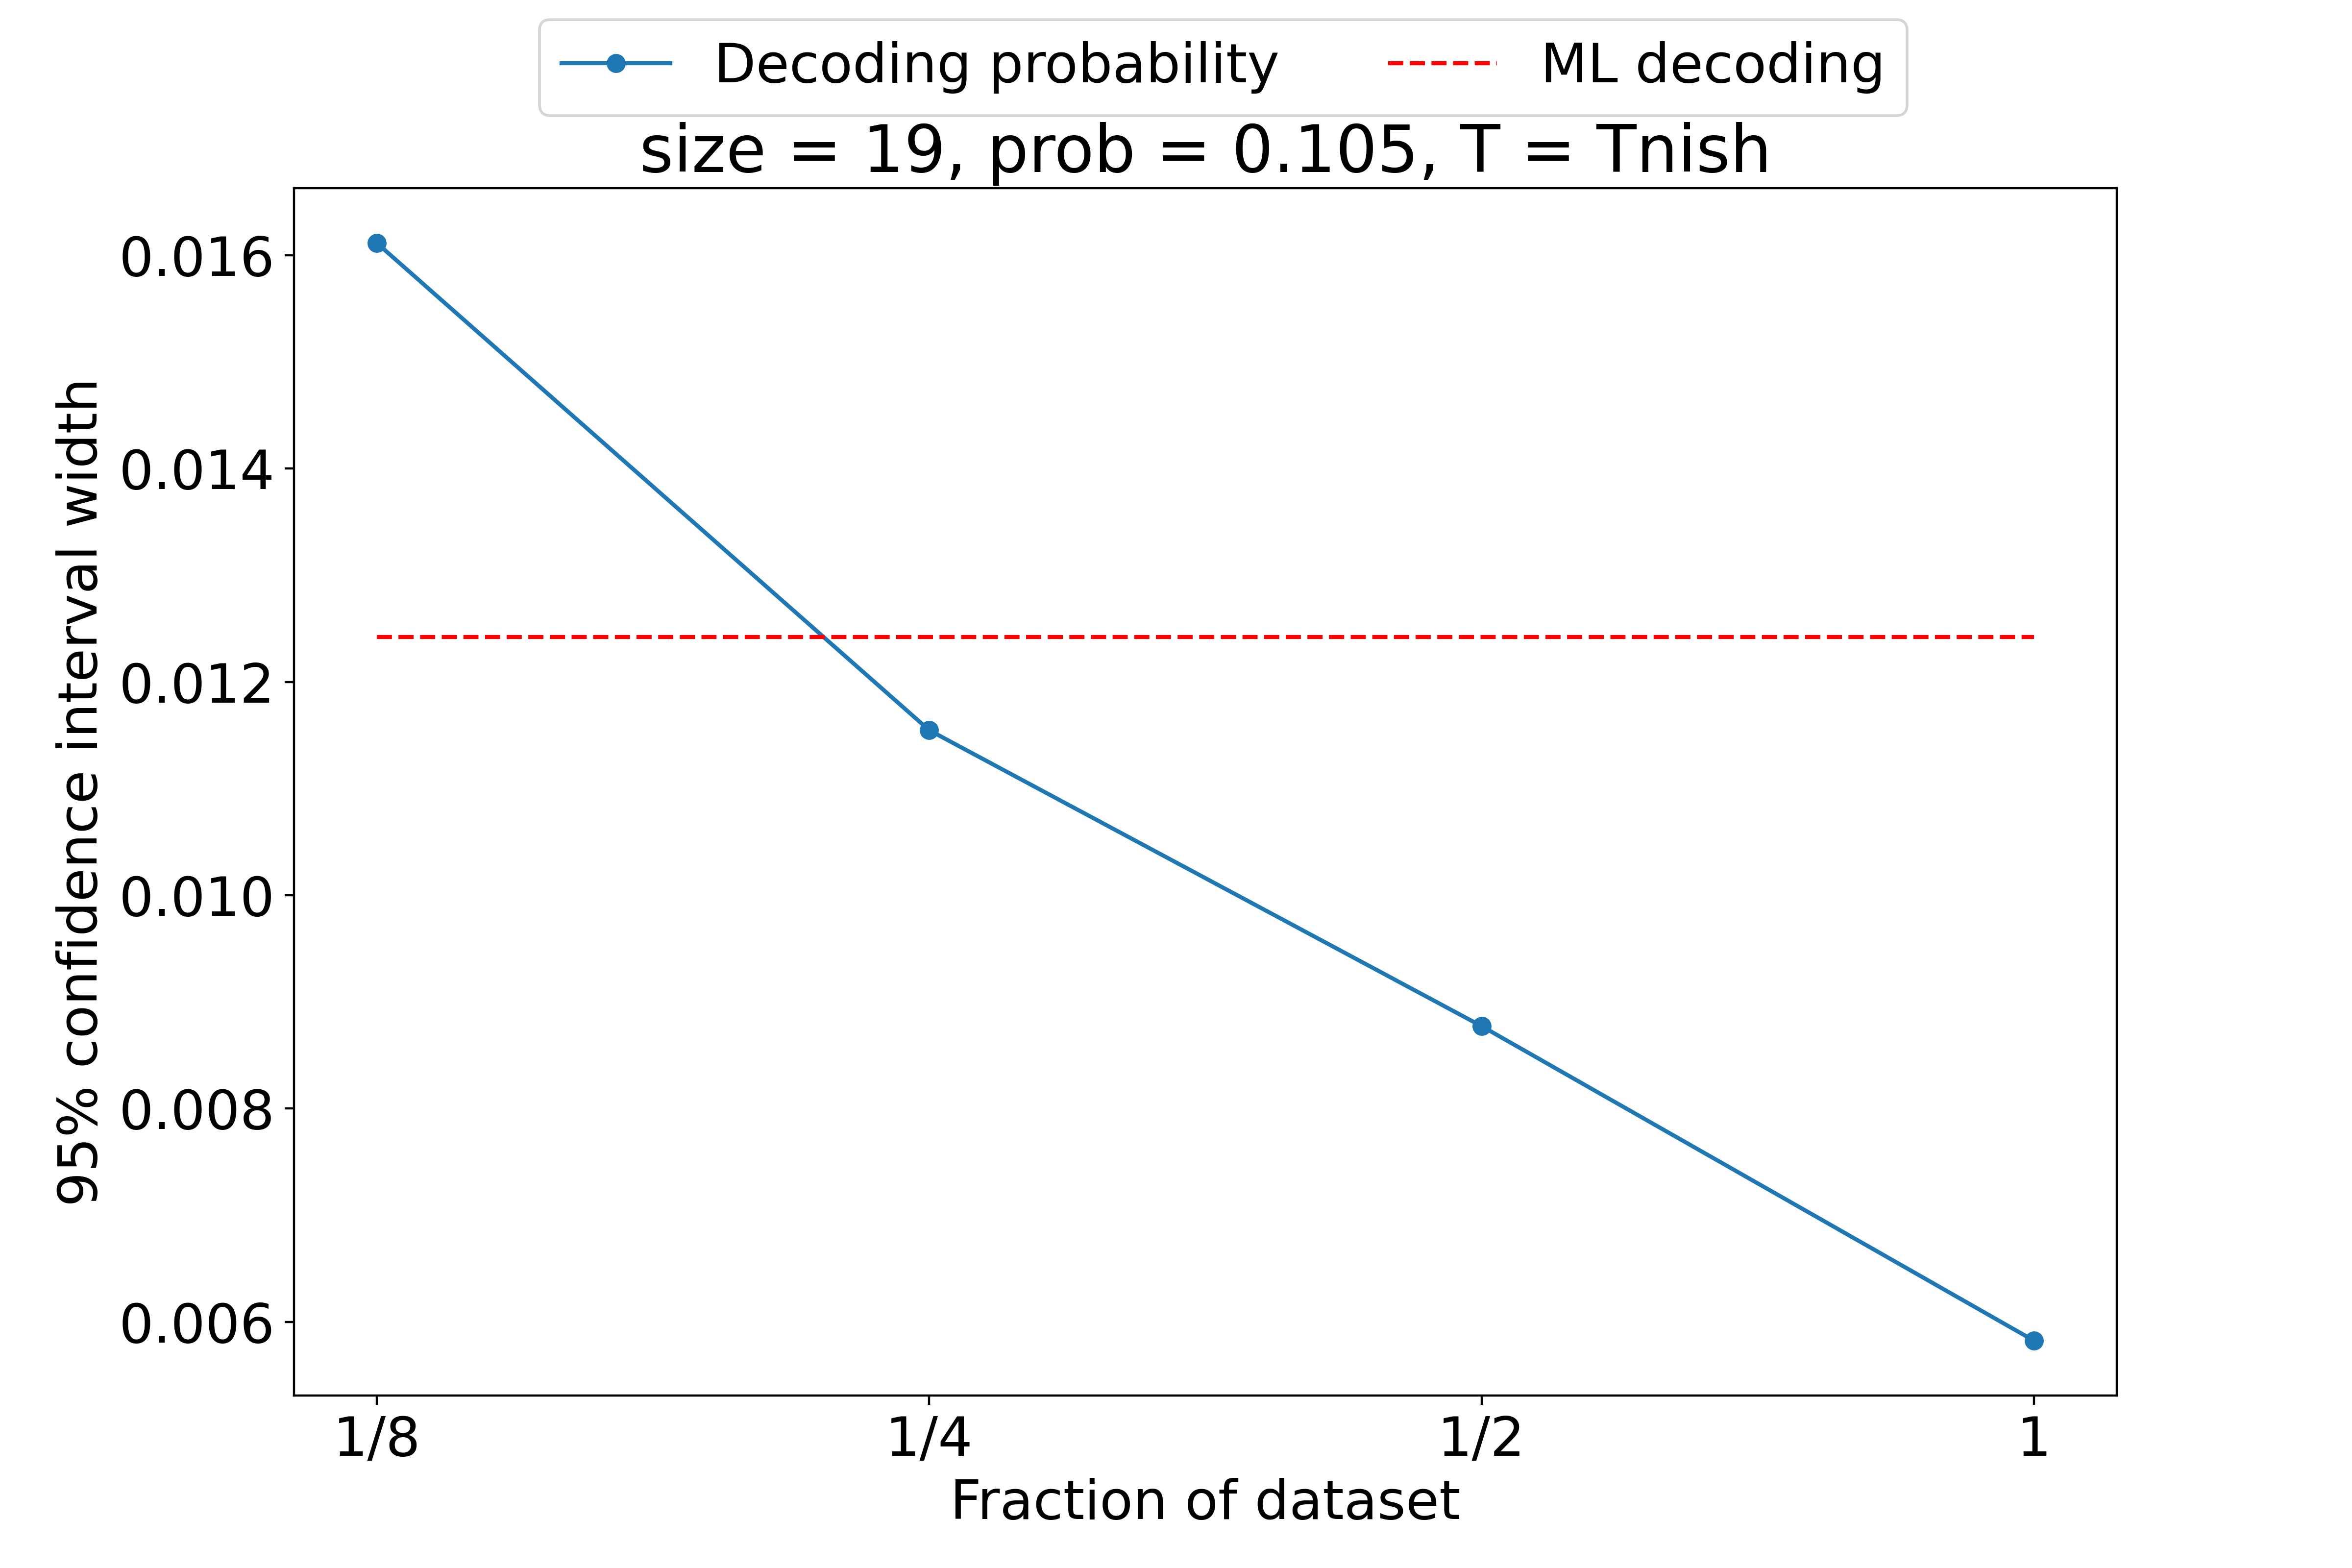
\includegraphics[width=0.5\linewidth]{fig/CIwidth.png}
		% \caption{Comparison of $95\%$ confidence interval width between decoding probability and max Z decoding with varying sample sizes for the calculation of the decoding probability}
	\end{figure}
\end{frame}

\begin{frame}{Preliminary Results}
	\begin{figure}[h!]
		\centering
		\begin{minipage}{0.45\textwidth}
			\centering
			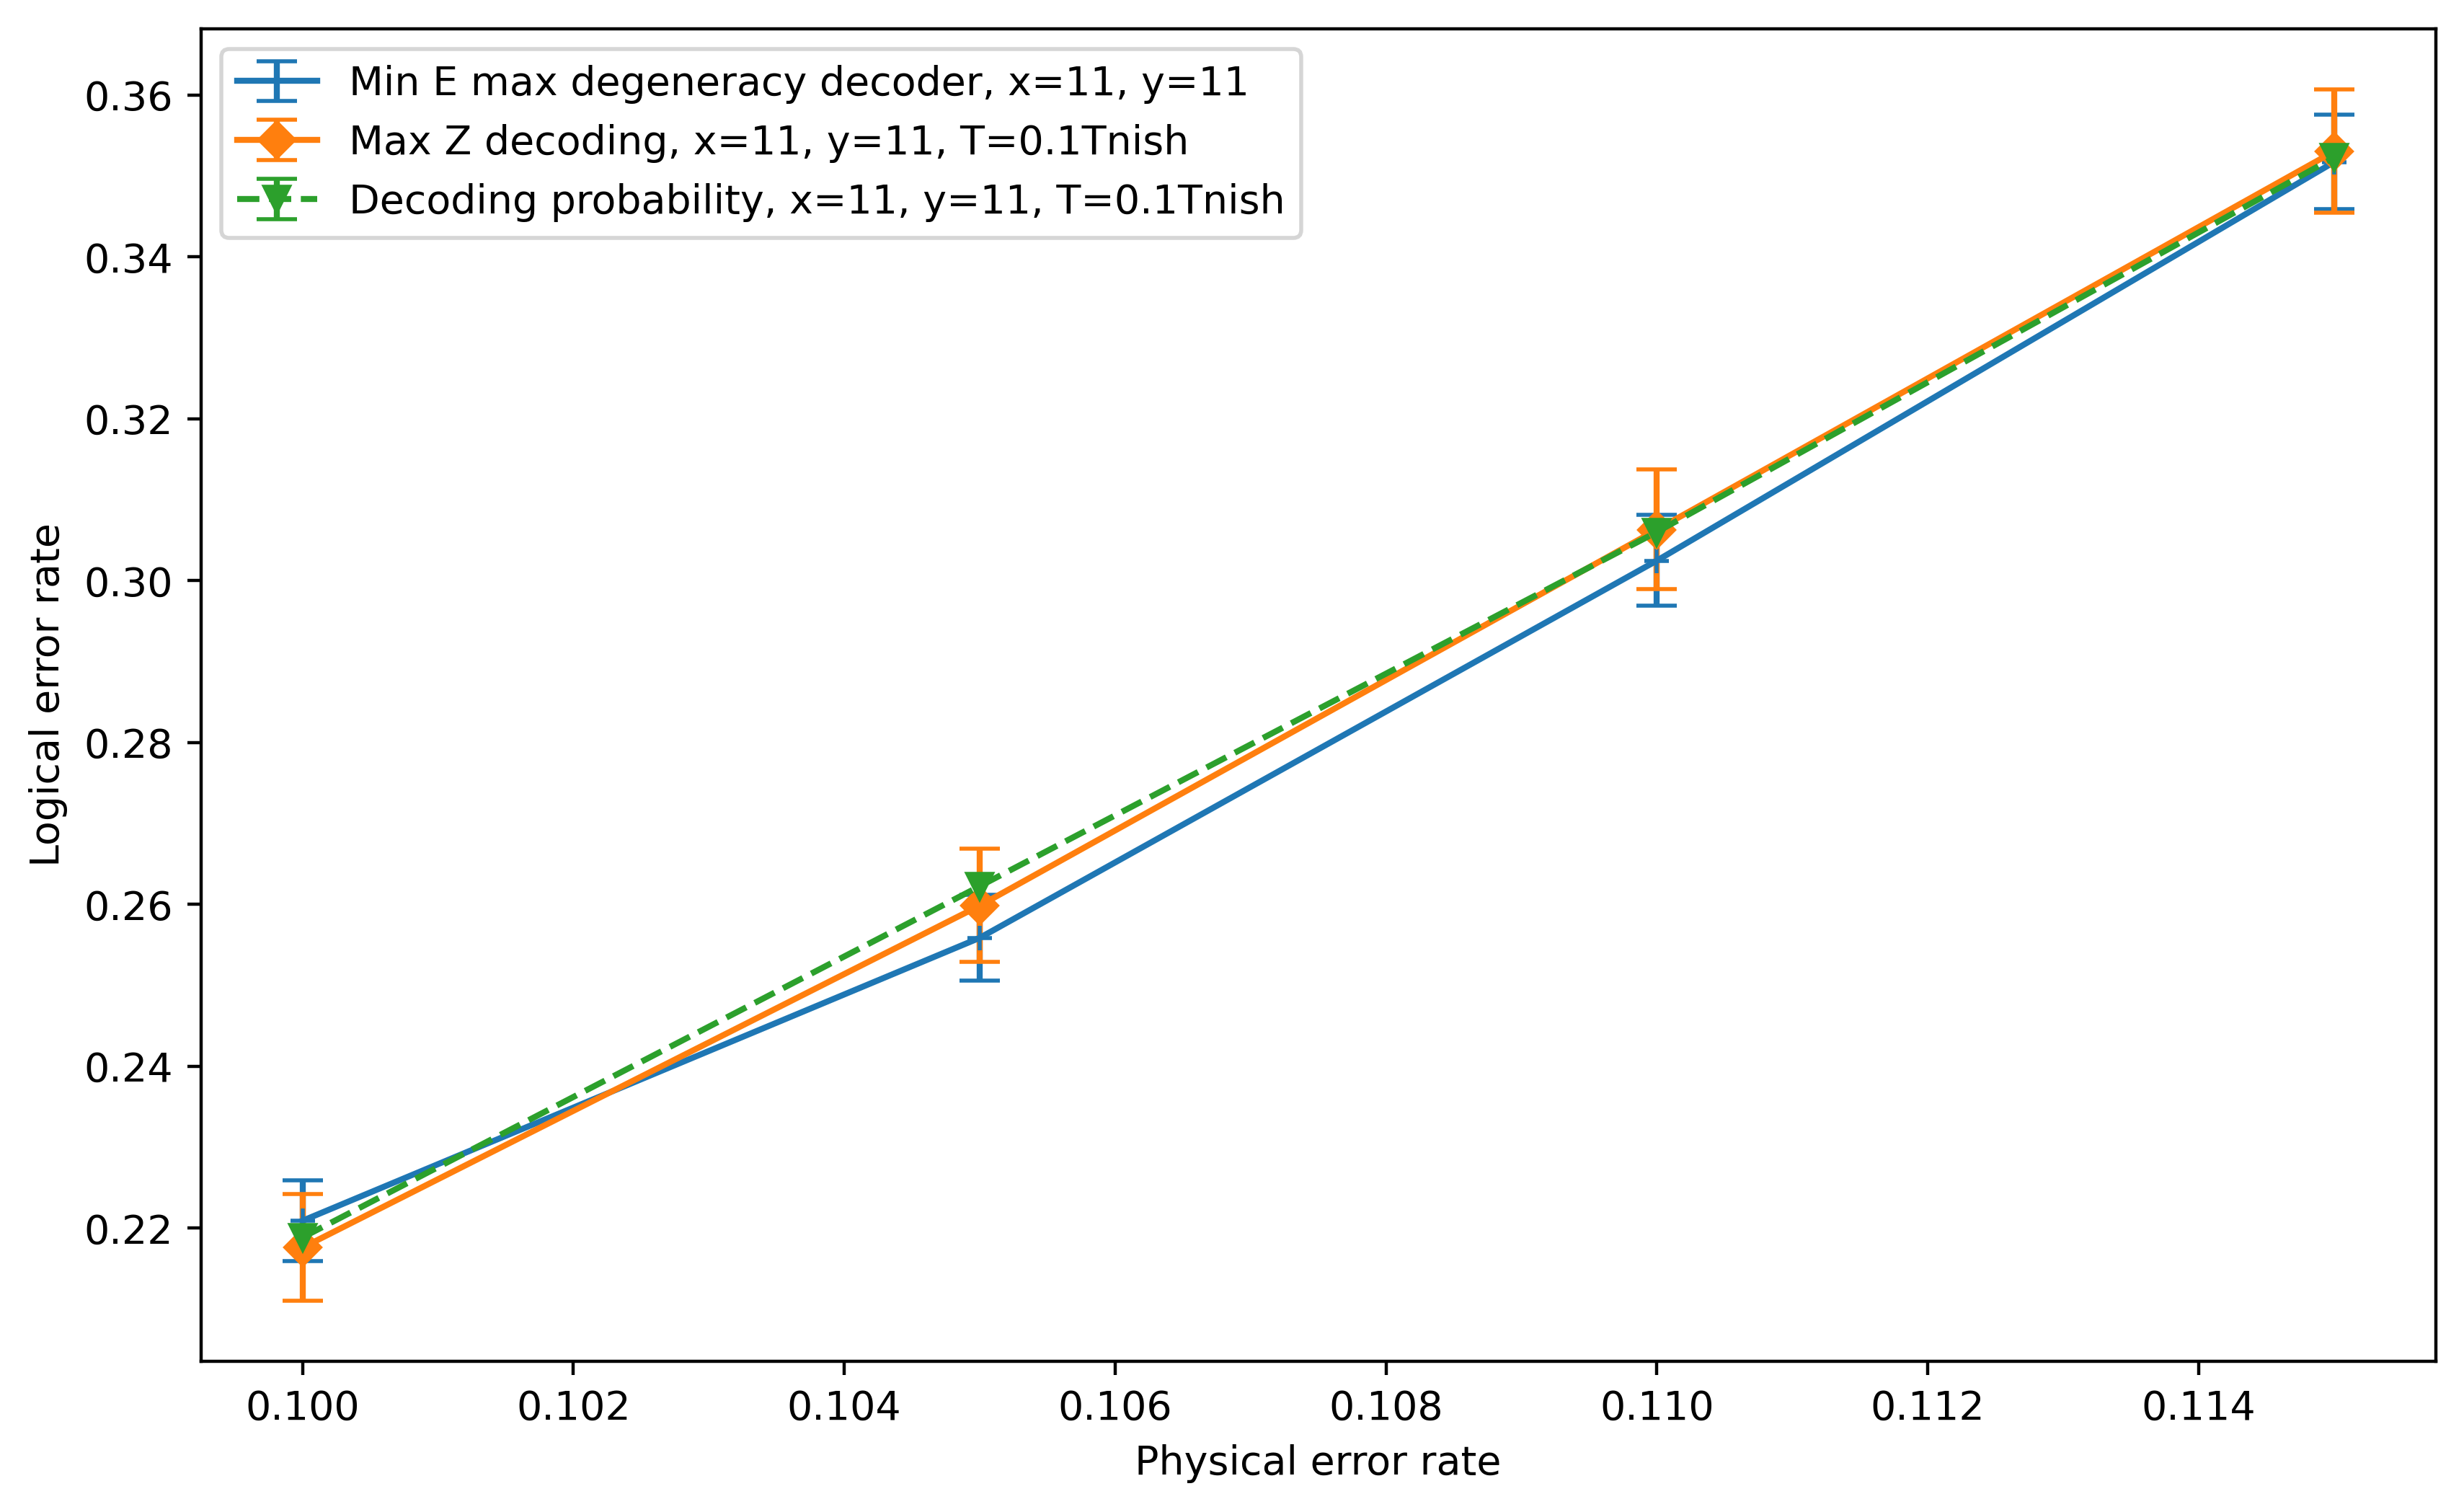
\includegraphics[width=\textwidth]{fig/MineEMaxG_DecProb01_LowTMaxZ_x11.png}
			\caption{Max Z decoding at low $T=0.1T_{\text{Nish}}$ reduces to max degeneracy ground state decoding for odd size $x=11$}
		\end{minipage} \hfill
		\begin{minipage}{0.45\textwidth}
			\centering
			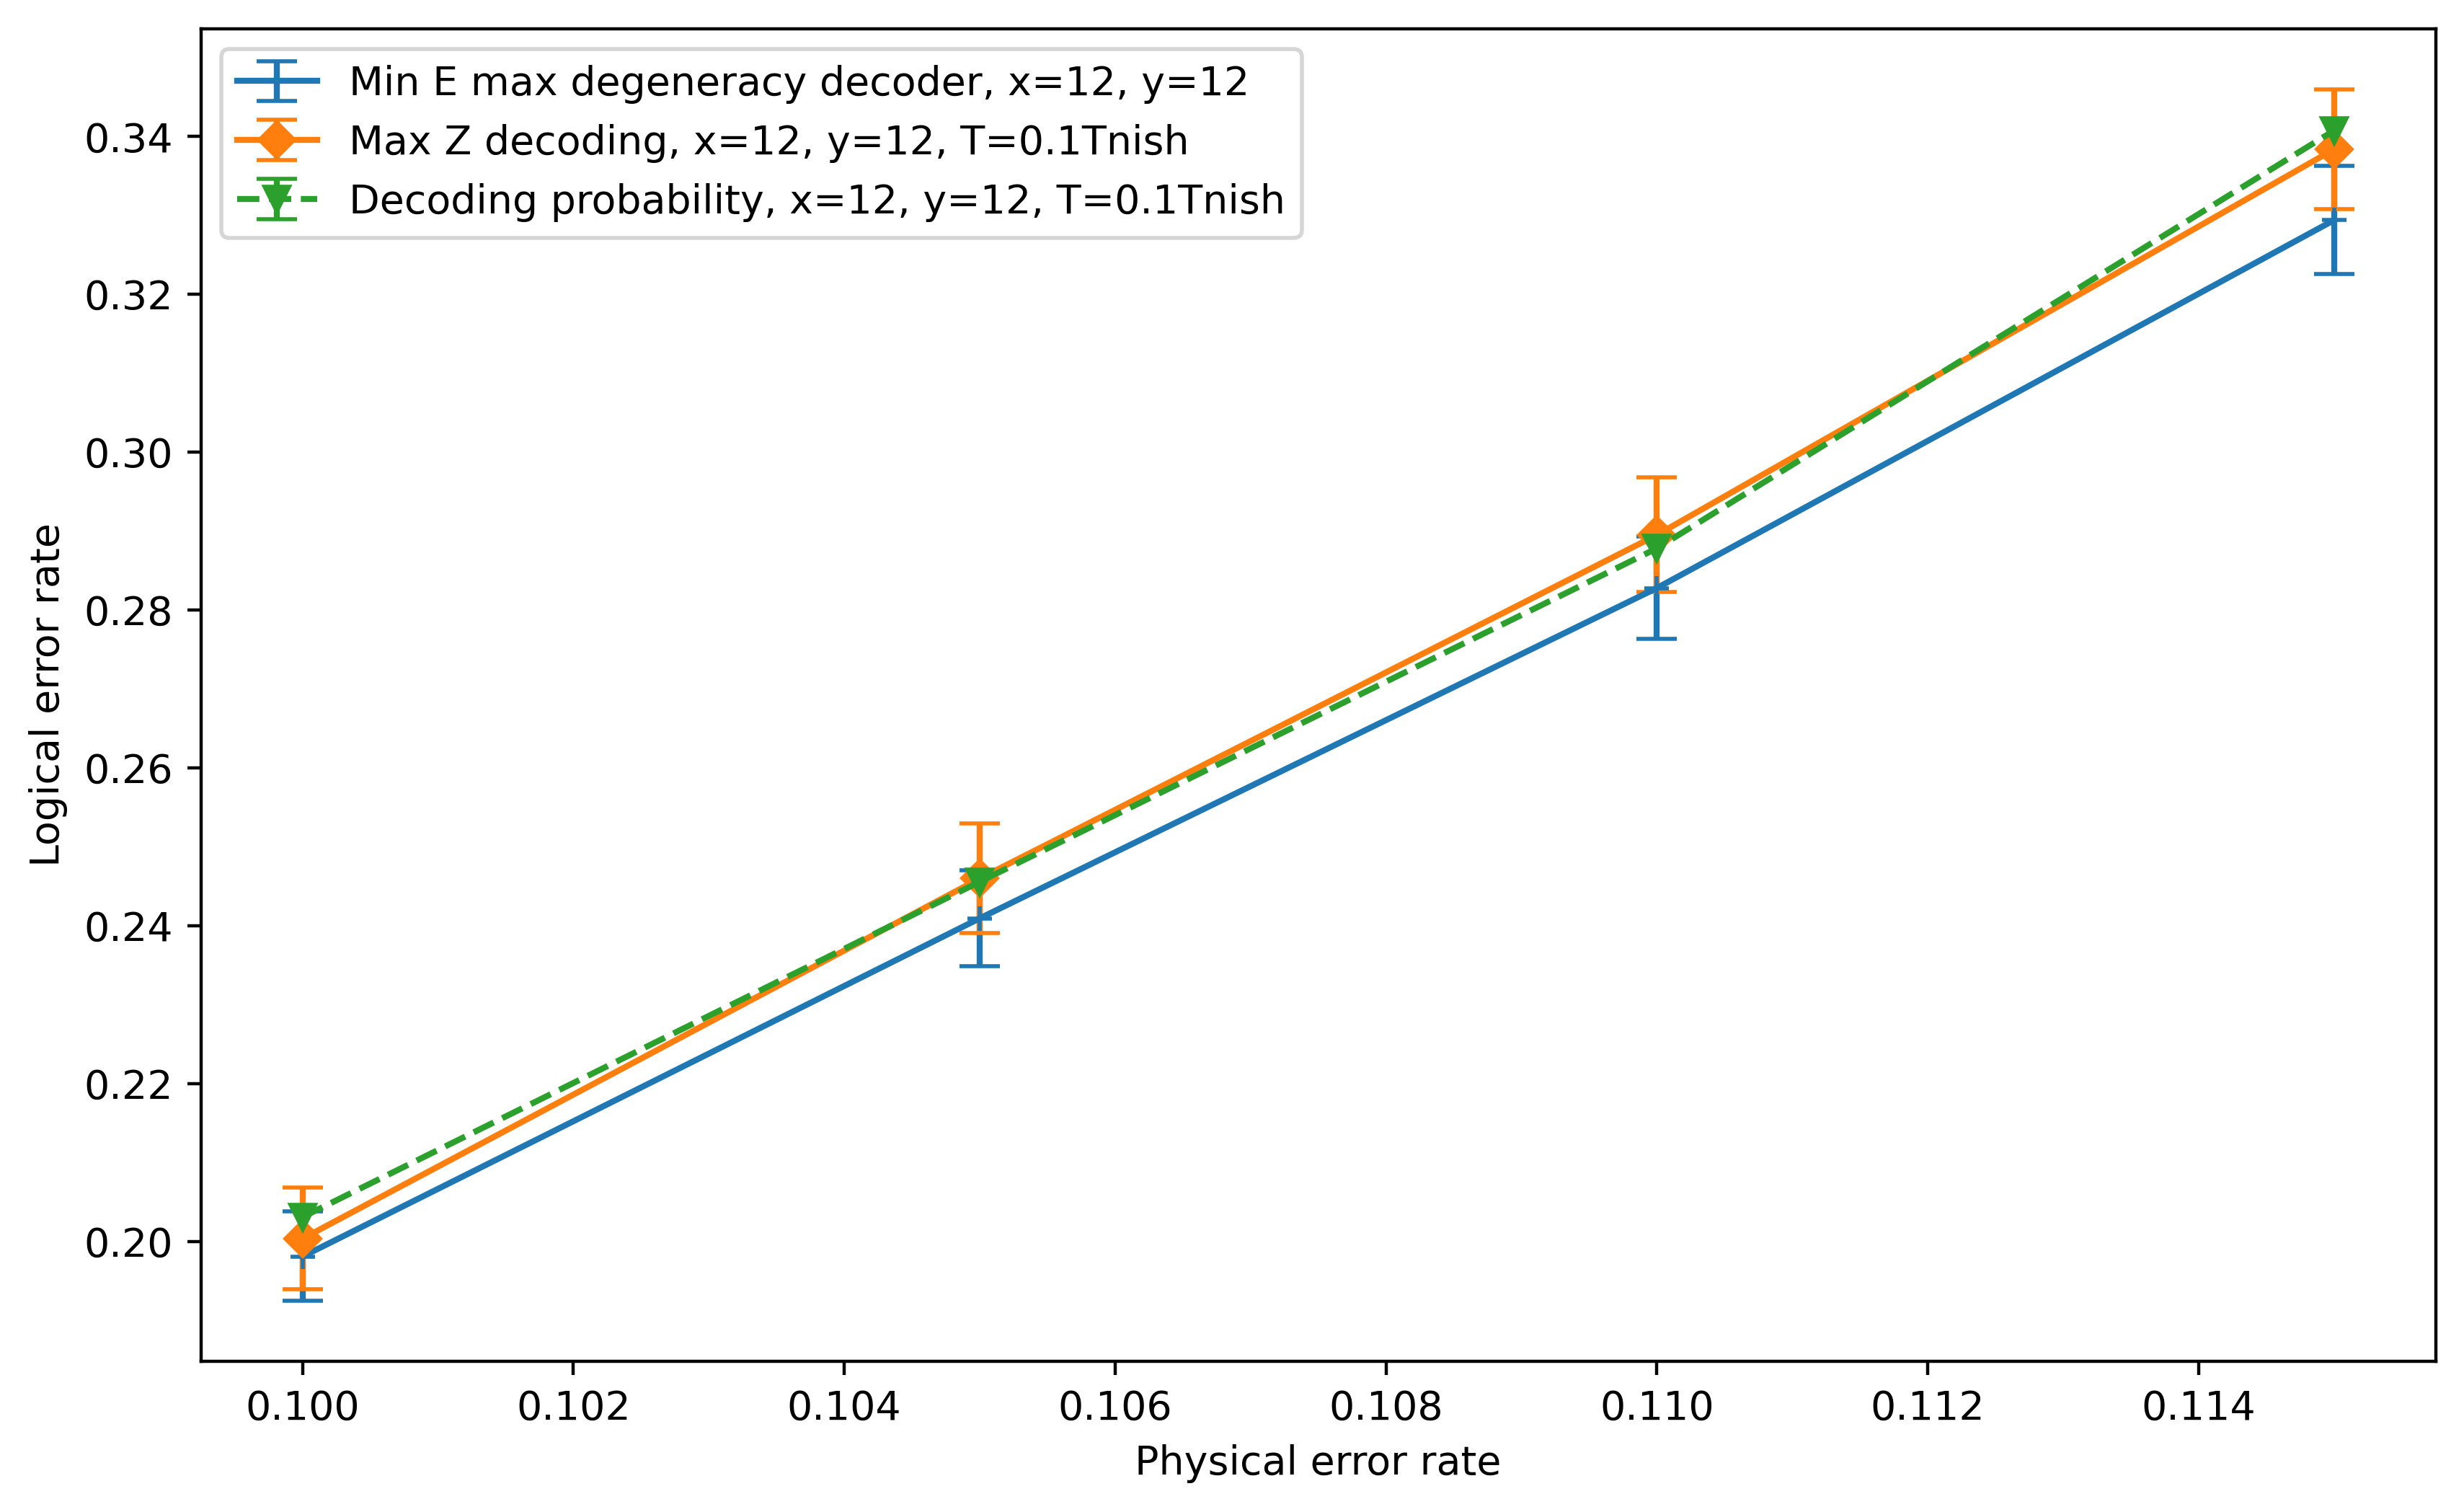
\includegraphics[width=\textwidth]{fig/MineEMaxG_DecProb01_LowTMaxZ_x12.png}
			\caption{Max Z decoding at low $T=0.1T_{\text{Nish}}$ reduces to max degeneracy ground state decoding for even size $x=12$}
		\end{minipage}
	\end{figure}
\end{frame}

\begin{frame}{Preliminary Results}
	\center
	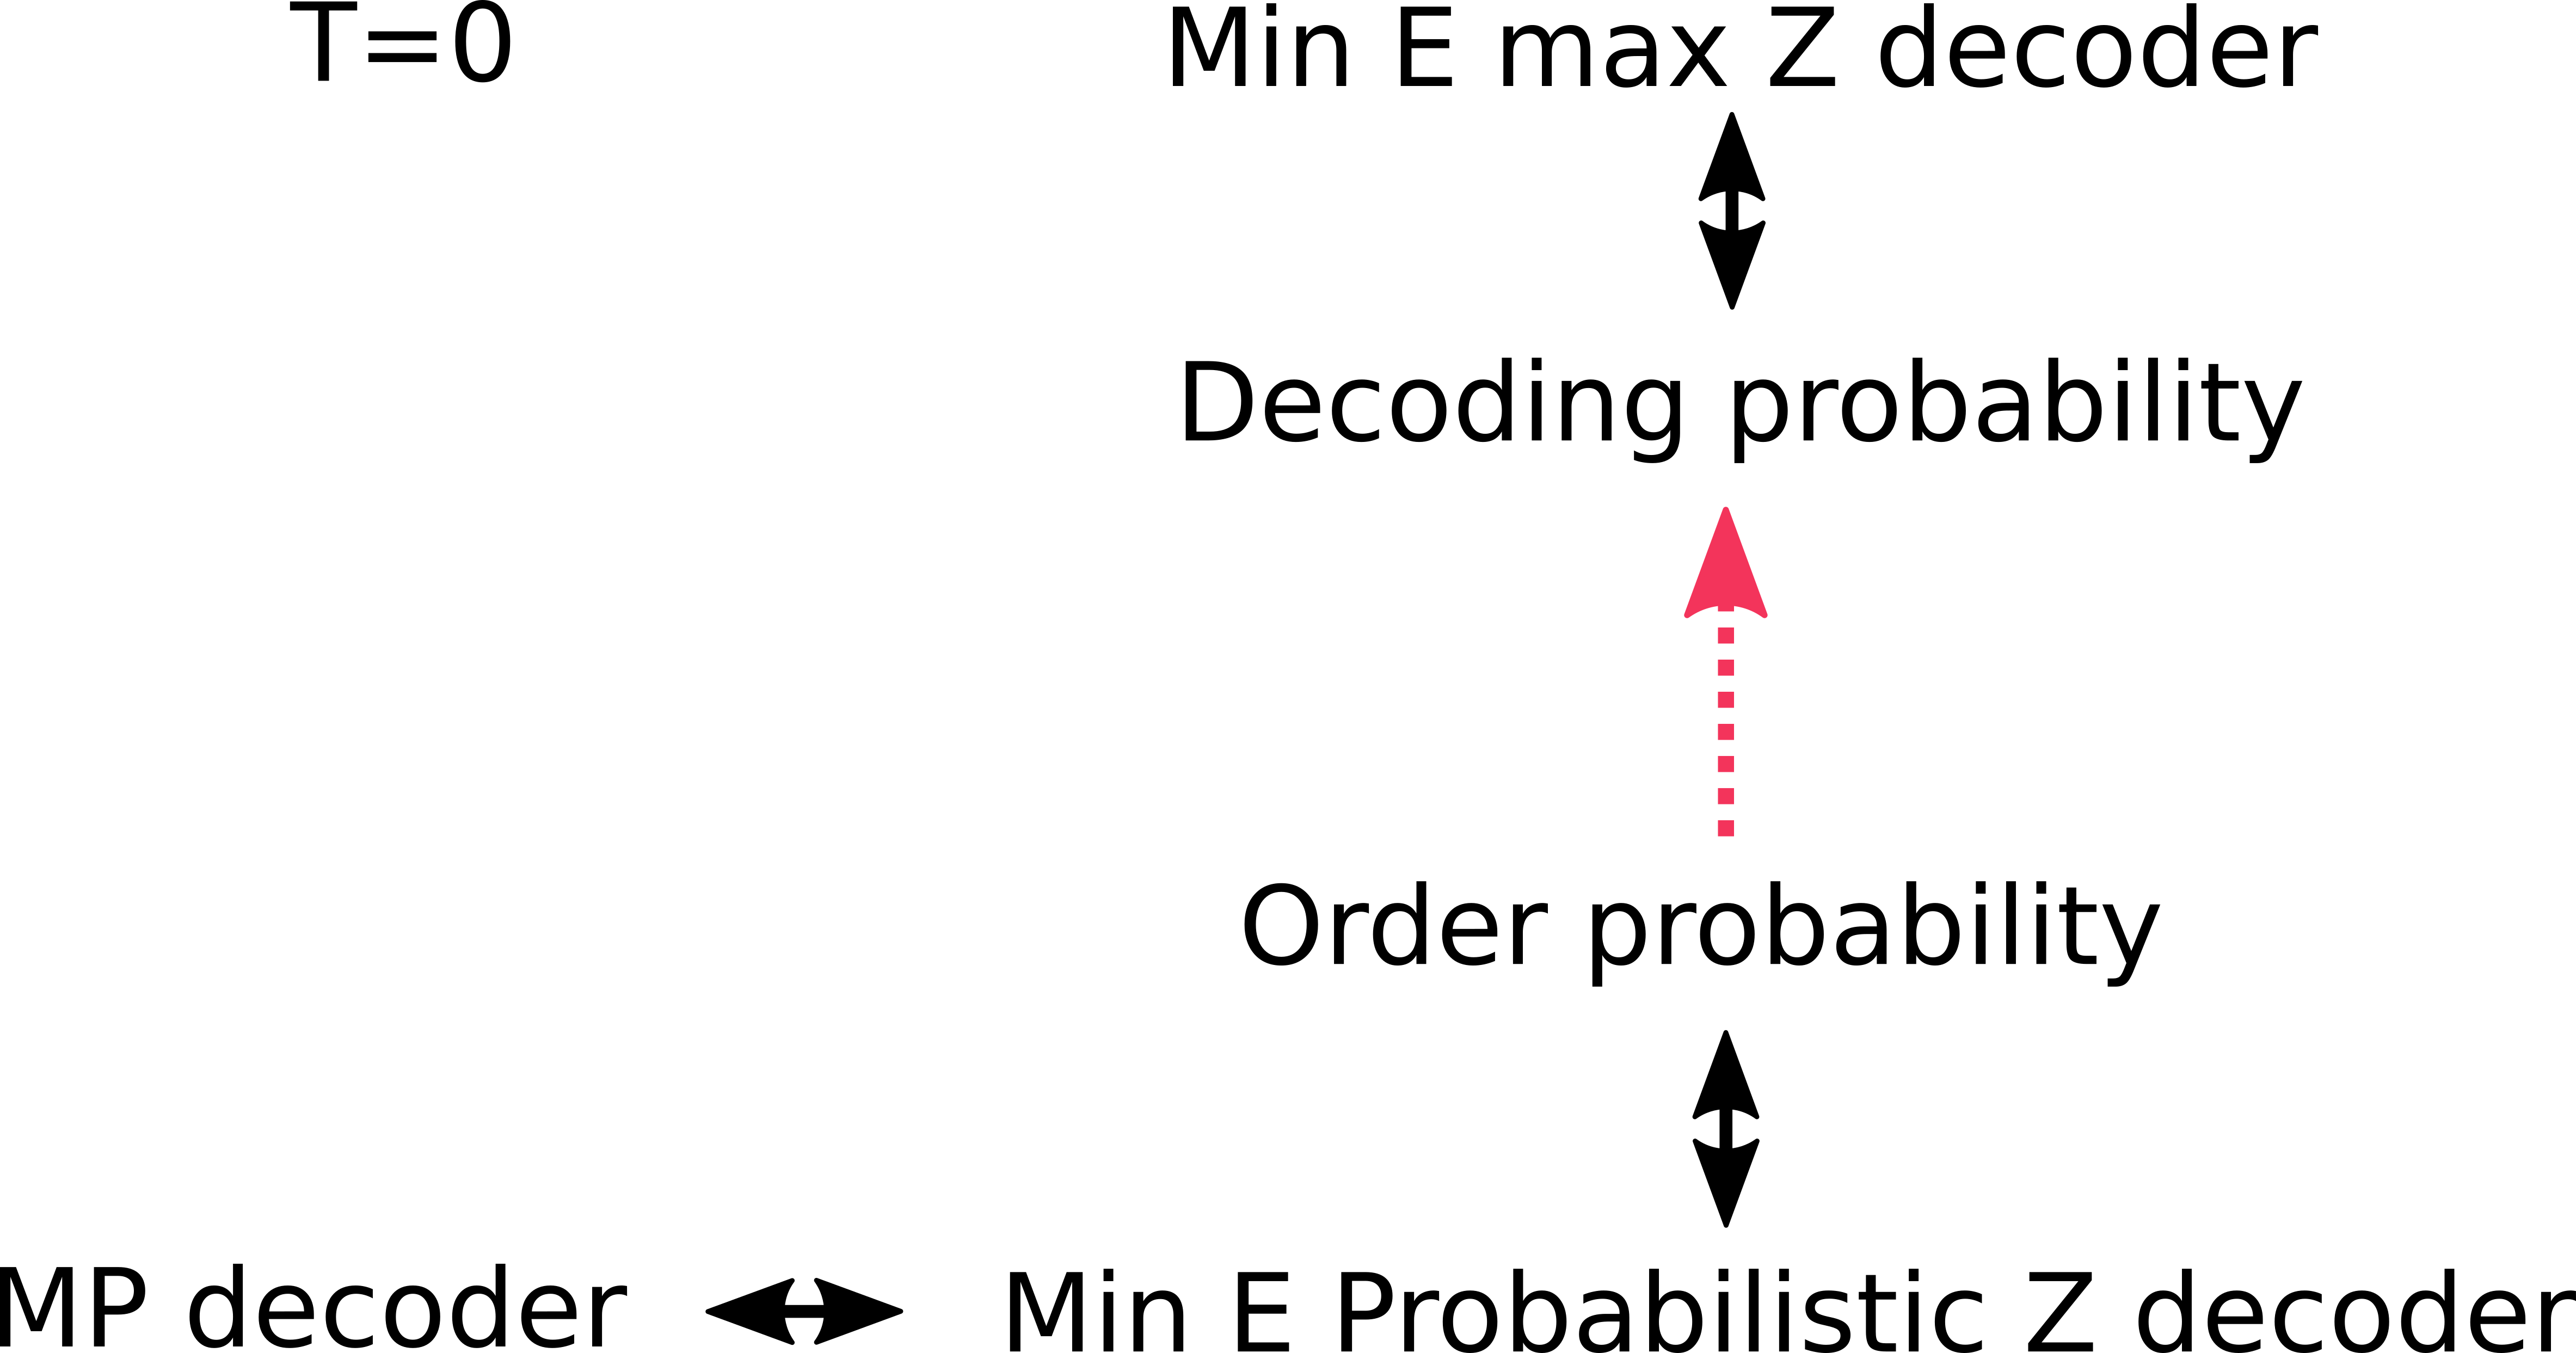
\includegraphics[width=0.7\textwidth]{fig/Optimization_potential.png}
\end{frame}


\begin{frame}{Conclusion and Outlook}
	\begin{textblock*}{14cm}(1.5cm,2cm)
		\raisebox{-0.5cm}{
\includegraphics[width=0.15\textwidth]{fig/Noise.png}}
		\begin{tikzpicture}[overlay]
			\draw[->, line width=0.8mm, black] (0.5, 0.1) -- (4,0.1);
			\draw[-, line width=0.8mm, black] (0.5, 0.3) -- (0.5,-0.1);
		\end{tikzpicture}
		\hspace{4.5cm}
		Optimal code performance estimate
	\end{textblock*}
	\vspace{3cm}
	\begin{itemize}
		\item \textbf{WL implementation:} Flexible but slow
		\item \textbf{FKT implementation:} Fast but not flexible
		\item \textbf{Decoder Optimization:} MWPM decoder can be enhanced by taking degeneracy of ground states into account
		\item \textbf{Near future:} TN implementation
		\item \textbf{Further:} More realistic noise model, color codes towards quantum algorithms
	\end{itemize}
\end{frame}

% conclusion + success metrics
% outlook
% make literature appear with name and year
% only info which I need and speak about
% union find in experimental usage
% how does belief propagation work
% scales for real time decoding




\begin{frame}
	\begin{center}
		{\huge\textbf{Thank you for your attention!}}
	\end{center}
\end{frame}

\printbibliography

\end{document}



% \begin{frame}{Recent advancements in QEC}
% 	\begin{tcolorbox}[colback=osakared!5!white, colframe=osakared, width=13cm, arc=2mm]
% 		\textbf{Google Quantum AI} Performed quantum memory experiments with surface codes below the error correction threshold.
% 	\end{tcolorbox}
% 	\vspace{10pt}
% 	$\Rightarrow$ Their hardware is in regime where code performance can be increased by increased system size\\
% 	\pause
% 	\vspace{10pt}
% 	Moreover they were able to improve the decoder performance by adapting to device noise.
% 	% The scaling of the physical qubit count from 72 to 101 qubits resulted in a suppression of the logical error rate by a factor of roughly two. \\
% 	% their optimized mwpm decoder was able to decode in real time while a neural network decoder only acted as offline decoder due to fast processor cycle duration
% \end{frame}

% \begin{frame}{Problem statement}
% 	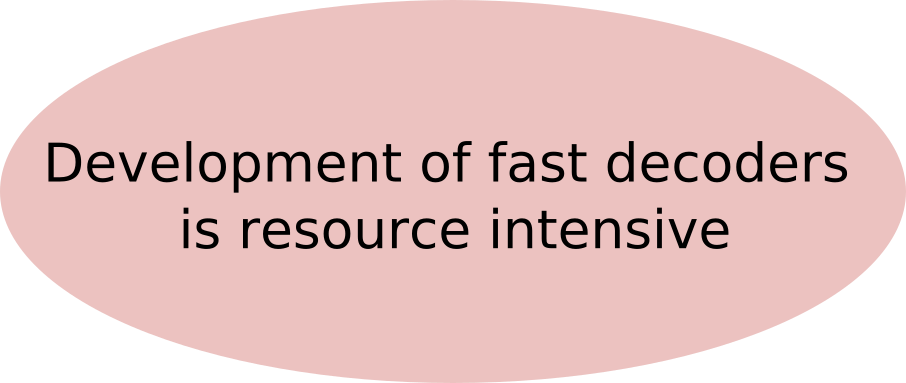
\includegraphics[width=0.4\textwidth]{fig/resource_intensive_decoder_dev.png}
% 	\only<1>{\hspace{20pt}\raisebox{35pt}{$\huge \Rightarrow$ \textbf{Only do it for promising codes}}}
% 	\only<2->{
% 		\hspace{2pt}
% 		\raisebox{18pt}{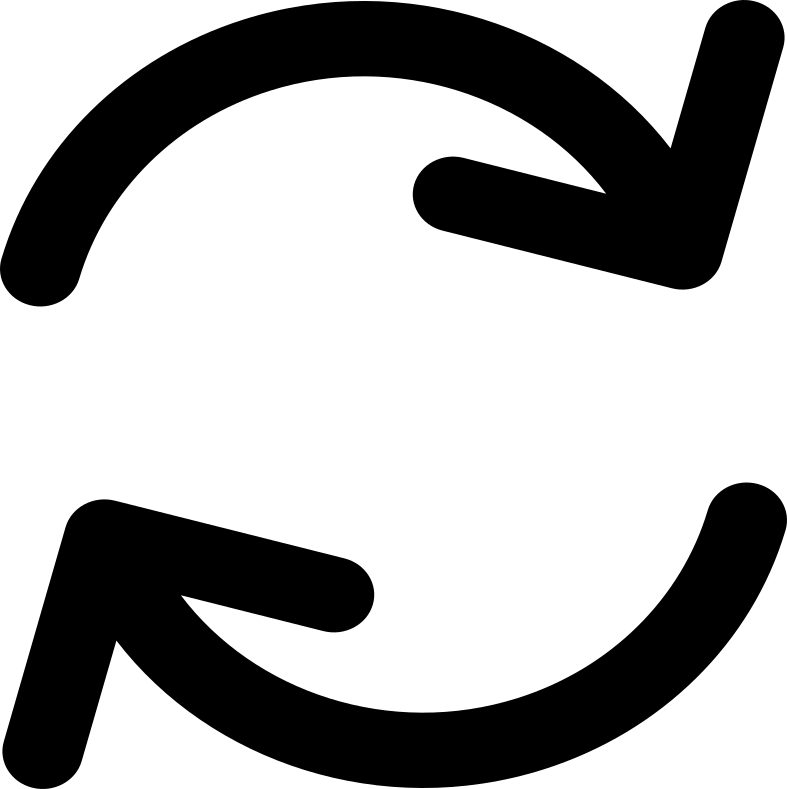
\includegraphics[width=0.08\textwidth]{fig/arrows.png}}
% 		\hspace{5pt}
% 		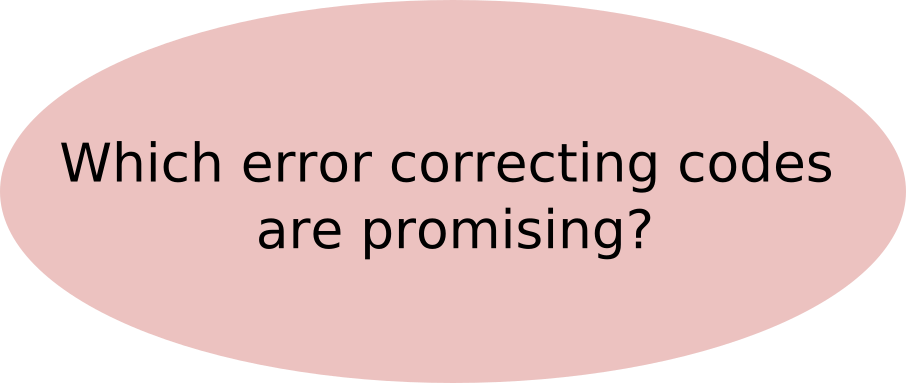
\includegraphics[width=0.4\textwidth]{fig/promising_codes.png}\\
% 	}
% 	\vspace{10pt}
% 	\only<3->{
% 	\textbf{Optimal code performance estimates can aid this process!}
% 	\begin{itemize}
% 		\only<3->{\item \textbf{Code selection:} Hardware specific simulation of optimal code performance makes error correcting codes comparable.}
% 		\only<4>{\item \textbf{Decoder optimization:} Estimation of optimal code performance shows upper limit for decoder optimization.}
% 	\end{itemize}
% 	}
% \end{frame}

% \begin{frame}{Preliminary Results}
% 	\only<1->{
% 	\begin{itemize}
% 		\only<1->{\item Developed a hardware adaptive framework for optimal code performance estimation}
% 		\only<2->{\item Applied framework to estimate optimal performance of the toric code under bitflip noise}
% 	\end{itemize}
% 	}
% 	\pause
% 	\vspace{-15pt}
% 	\begin{center}
% 		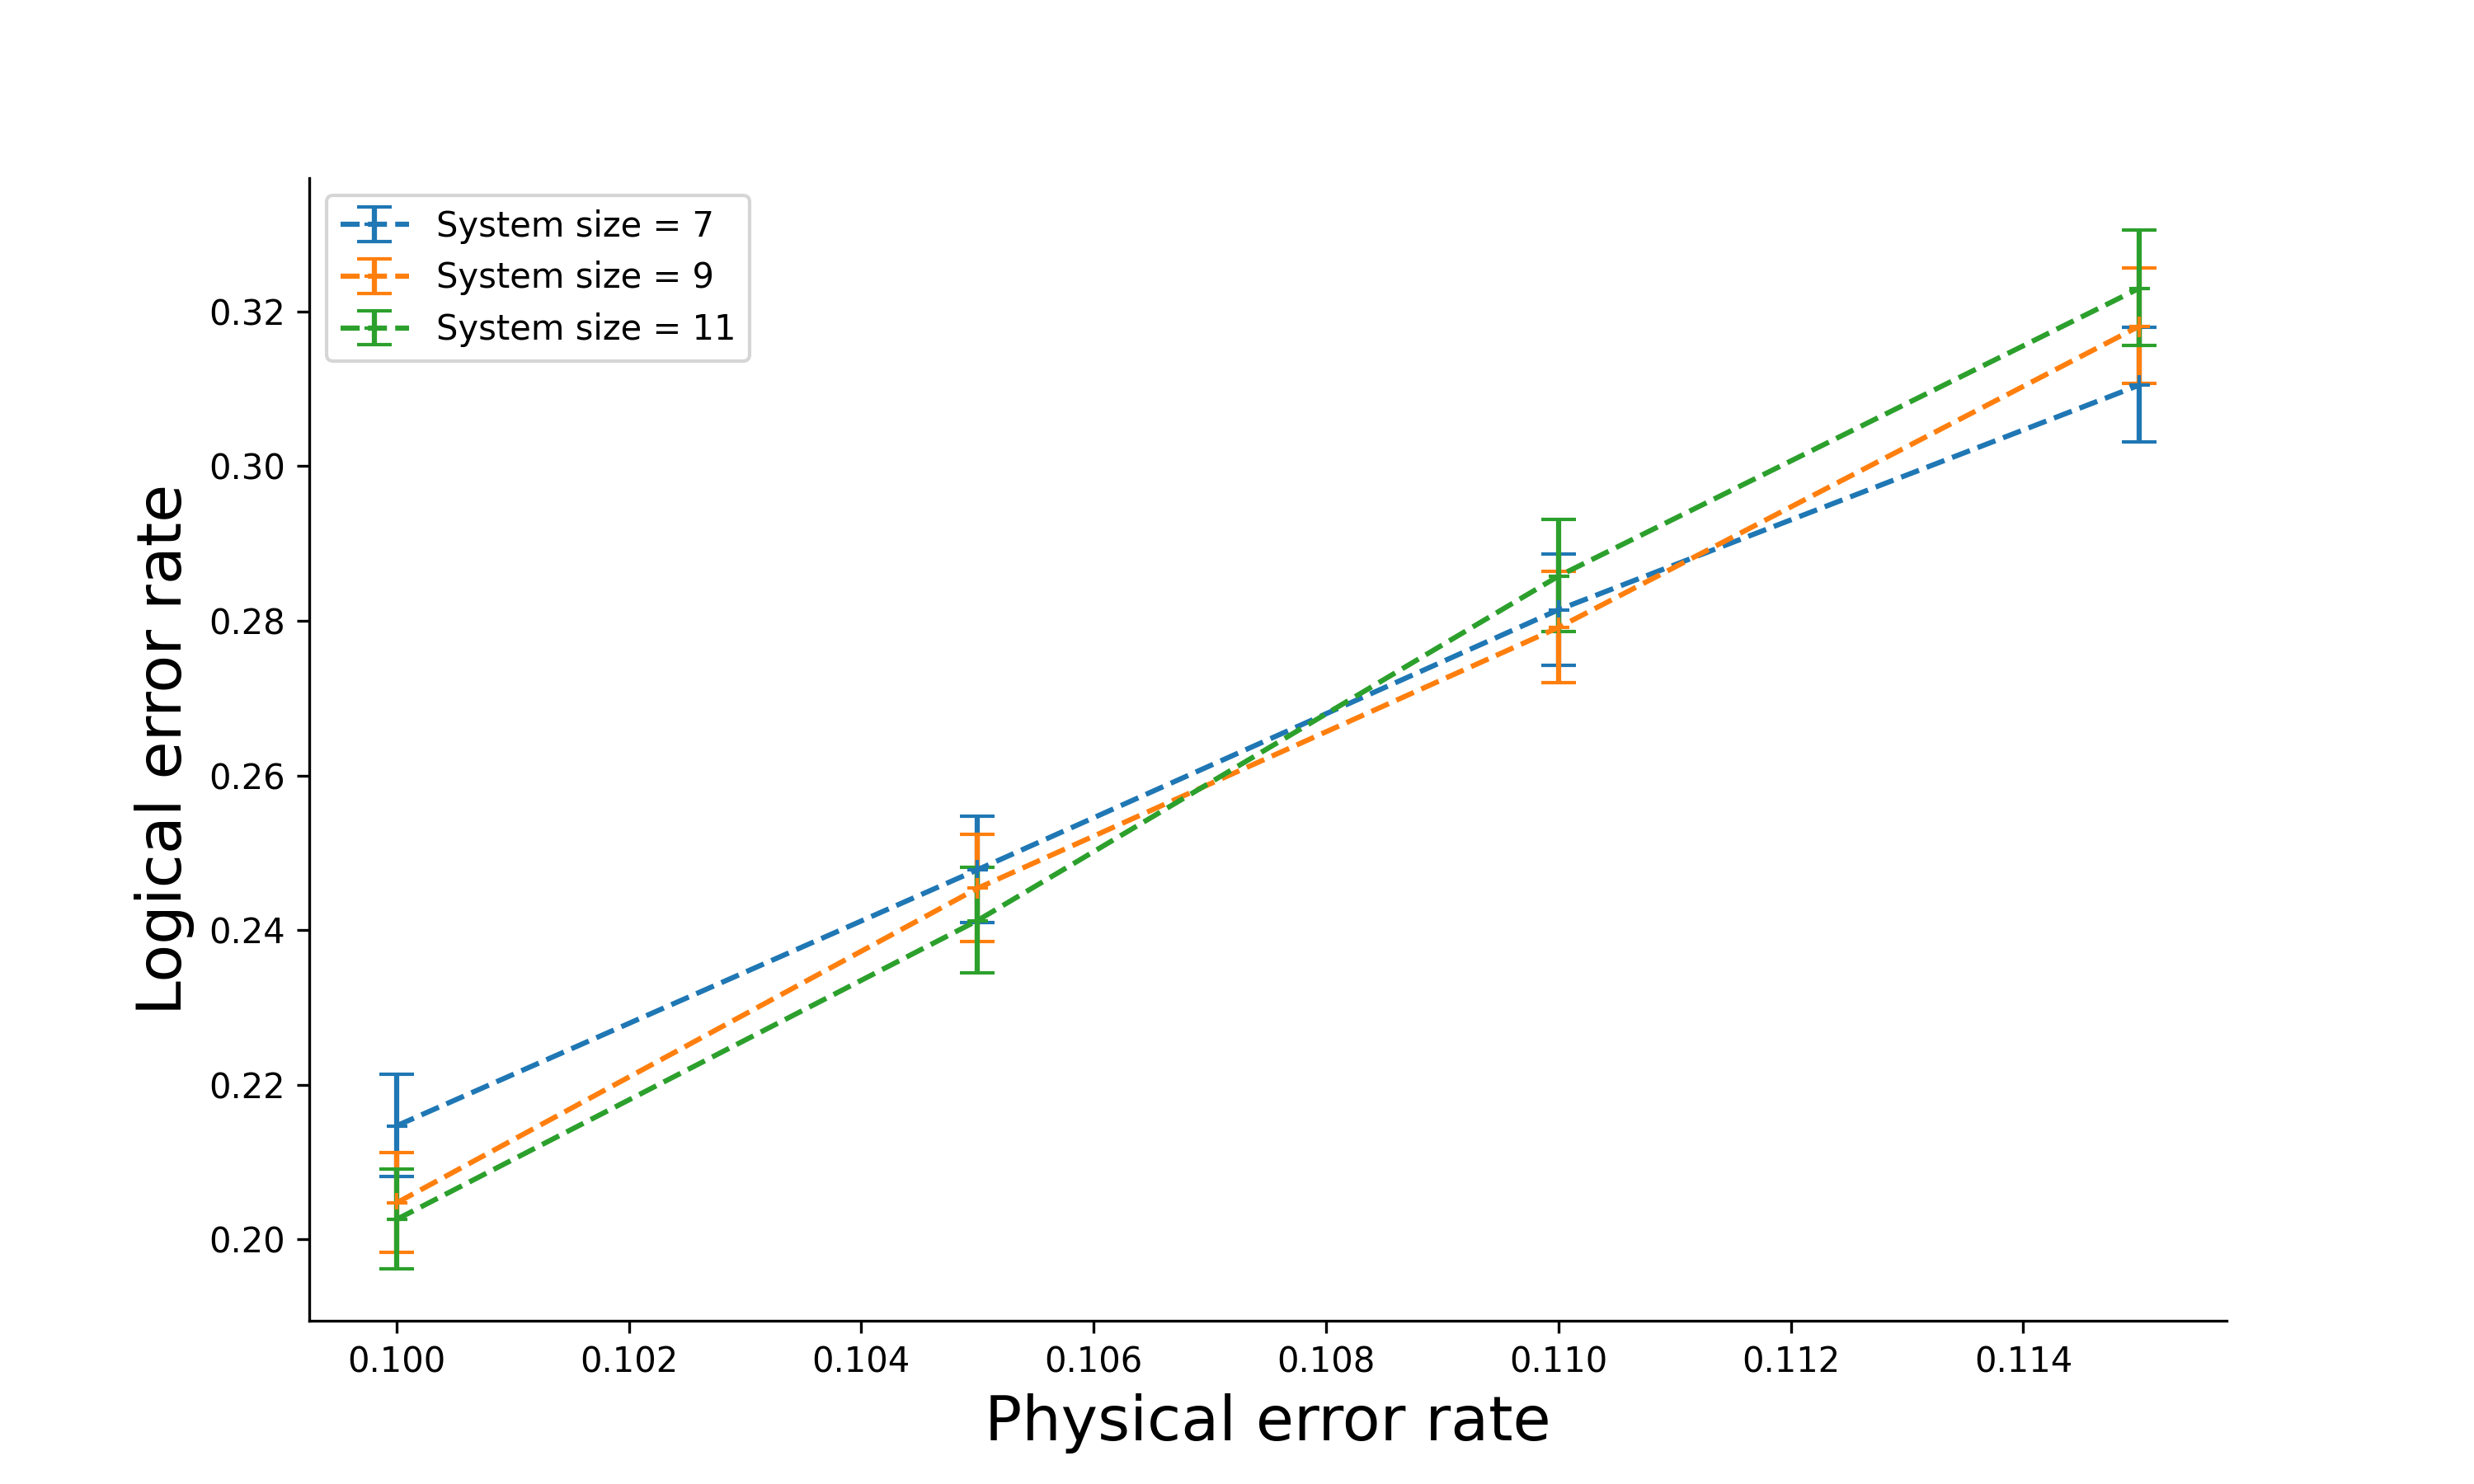
\includegraphics[width=0.6\linewidth]{fig/FKT threshold Temp=1.0.png}
% 	\end{center}
% 	% We produced estimates for the error correction threshold of the toric code under bitflip noise. \\
% 	% Here we can clearly see the two regimes which are governed by different scaling behavior with the qubit count of the error correcting code. \\
% \end{frame}

% \begin{frame}{Preliminary Results}
% 	Improved performance of a fast decoder and compared to optimal decoder performance: % maximum likelihood decoding is NP hard
% 	\begin{center}
% 		\includegraphics[width=0.6\linewidth]{fig/Improved decoder 10.png}
% 	\end{center}
% \end{frame}

% \begin{frame}{Preliminary Results}
% 	Investigation of noise informed decoder:
% 	\begin{center}
% 		\includegraphics[width=0.5\linewidth]{fig/noise_aware.png}
% 	\end{center}
% \end{frame}

% \begin{frame}{Summary}
% 	\begin{center}
% 		\includegraphics[width=0.8\linewidth]{fig/summary.png}
% 	\end{center}
% \end{frame}

% \begin{frame}{Work plan}
% 	\begin{table}[h]
% 		\fontsize{8pt}{9pt}\selectfont
% 		\center
% 		{\renewcommand{\arraystretch}{2}
% 		\begin{tabular}{l@{\hspace{1em}}p{4.5cm}p{3cm}l@{\hspace{1em}}p{1.7cm}}
%             \toprule
%             Authorship & Title & Type  & Year & Status   \\
%             \midrule
%             1st-author & Estimating optimal performance in stabilizer and subsystem codes & Physical Review A & 2025 & submission March-April \\
% 			co-author & Parallelization of Shor's algorithm & IEEE Transactions on Quantum Engineering & 2025 & submission February \\
%             to be discussed & Extending current results to realistic noise models & Journal & 2025-26 & Future work \\
% 			to be discussed & QuaSA: Error dynamics of Quantum Memory & Journal & 2026 & Future work \\
%             \bottomrule
%         \end{tabular}
% 		}
% 	\end{table} \vfill
% \end{frame}
